% ******************************* PhD Thesis Template **************************
% Please have a look at the README.md file for info on how to use the template

\documentclass[a4paper,12pt,times,numbered,print,index]{Classes/PhDThesisPSnPDF}

%\documentclass[a4paper,12pt,times,numbered,print,index, chapter]{Classes/PhDThesisPSnPDF}
% ******************************************************************************
% ******************************* Class Options ********************************
% *********************** See README for more details **************************
% ******************************************************************************

% `a4paper'(The University of Cambridge PhD thesis guidelines recommends a page
% size a4 - default option) or `a5paper': A5 Paper size is also allowed as per
% the Cambridge University Engineering Deparment guidelines for PhD thesis
%
% `11pt' or `12pt'(default): Font Size 10pt is NOT recommended by the University
% guidelines
%
% `oneside' or `twoside'(default): Printing double side (twoside) or single
% side.
%
% `print': Use `print' for print version with appropriate margins and page
% layout. Leaving the options field blank will activate Online version.
%
% `index': For index at the end of the thesis
%
% `draftclassic': For draft mode without loading any images (same as draft in book)
%
% `draft': Special draft mode with line numbers, images, and water mark with
% timestamp and custom text. Position of the text can also be modified.
%
% `abstract': To generate only the title page and abstract page with
% dissertation title and name, to submit to the Student Registry
%
% `chapter`: This option enables only the specified chapter and it's references
%  Useful for review and corrections.
%
% ************************* Custom Page Margins ********************************
%
% `custommargin`: Use `custommargin' in options to activate custom page margins,
% which can be defined in the preamble.tex. Custom margin will override
% print/online margin setup.
%
% *********************** Choosing the Fonts in Class Options ******************
%
% `times' : Times font with math support. (The Cambridge University guidelines
% recommend using times)
%
% `fourier': Utopia Font with Fourier Math font (Font has to be installed)
%            It's a free font.
%
% `customfont': Use `customfont' option in the document class and load the
% package in the preamble.tex
%
% default or leave empty: `Latin Modern' font will be loaded.
%
% ********************** Choosing the Bibliography style ***********************
%
% `authoryear': For author-year citation eg., Krishna (2013)
%
% `numbered': (Default Option) For numbered and sorted citation e.g., [1,5,2]
%
% `custombib': Define your own bibliography style in the `preamble.tex' file.
%              `\RequirePackage[square, sort, numbers, authoryear]{natbib}'.
%              This can be also used to load biblatex instead of natbib
%              (See Preamble)
%
% **************************** Choosing the Page Style *************************
%
% `default (leave empty)': For Page Numbers in Header (Left Even, Right Odd) and
% Chapter Name in Header (Right Even) and Section Name (Left Odd). Blank Footer.
%
% `PageStyleI': Chapter Name next & Page Number on Even Side (Left Even).
% Section Name & Page Number in Header on Odd Side (Right Odd). Footer is empty.
%
% `PageStyleII': Chapter Name on Even Side (Left Even) in Header. Section Number
% and Section Name in Header on Odd Side (Right Odd). Page numbering in footer
%set the page style to have page number at bottom, titles at top as set out by NUIG guidelines(http://www.nuigalway.ie/media/graduatestudies/files/university_guidelines_for_research_degree_programmes.pdf): Pages must be numbered consecutively, with page numbers located centrally at the bottom, and chapter headers at the top, of each page
% Uncomment to change page style
\pagestyle{PageStyleII}

% ********************************** Preamble **********************************
% Preamble: Contains packages and user-defined commands and settings
% ******************************************************************************
% ****************************** Custom Margin *********************************

% Add `custommargin' in the document class options to use this section
% Set {innerside margin / outerside margin / topmargin / bottom margin}  and
% other page dimensions
\ifsetCustomMargin
  \RequirePackage[left=40mm,right=30mm,top=35mm,bottom=30mm]{geometry}
  \setFancyHdr % To apply fancy header after geometry package is loaded
\fi

% Add spaces between paragraphs
%\setlength{\parskip}{0.5em}
% Ragged bottom avoids extra whitespaces between paragraphs
\raggedbottom
% To remove the excess top spacing for enumeration, list and description
%\usepackage{enumitem}
%\setlist[enumerate,itemize,description]{topsep=0em}

% *****************************************************************************
% ******************* Fonts (like different typewriter fonts etc.)*************

% Add `customfont' in the document class option to use this section

\ifsetCustomFont
  % Set your custom font here and use `customfont' in options. Leave empty to
  % load computer modern font (default LaTeX font).
  %\RequirePackage{helvet}

  % For use with XeLaTeX
  %  \setmainfont[
  %    Path              = ./libertine/opentype/,
  %    Extension         = .otf,
  %    UprightFont = LinLibertine_R,
  %    BoldFont = LinLibertine_RZ, % Linux Libertine O Regular Semibold
  %    ItalicFont = LinLibertine_RI,
  %    BoldItalicFont = LinLibertine_RZI, % Linux Libertine O Regular Semibold Italic
  %  ]
  %  {libertine}
  %  % load font from system font
  %  \newfontfamily\libertinesystemfont{Linux Libertine O}
\fi

% *****************************************************************************
% **************************** Custom Packages ********************************

% ************************* Algorithms and Pseudocode **************************

%\usepackage{algpseudocode}


% ********************Captions and Hyperreferencing / URL **********************

% Captions: This makes captions of figures use a boldfaced small font.
%\RequirePackage[small,bf]{caption}

\RequirePackage[labelsep=space,tableposition=top]{caption}
\renewcommand{\figurename}{Fig.} %to support older versions of captions.sty


% *************************** Graphics and figures *****************************

%\usepackage{rotating}
%\usepackage{wrapfig}

% Uncomment the following two lines to force Latex to place the figure.
% Use [H] when including graphics. Note 'H' instead of 'h'
%\usepackage{float}
%\restylefloat{figure}

% Subcaption package is also available in the sty folder you can use that by
% uncommenting the following line
% This is for people stuck with older versions of texlive
%\usepackage{sty/caption/subcaption}
%\usepackage{subcaption}

% ********************************** Tables ************************************
\usepackage{booktabs} % For professional looking tables
\usepackage{multirow}

%\usepackage{multicol}
%\usepackage{longtable}
%\usepackage{tabularx}


% *********************************** SI Units *********************************
\usepackage{siunitx} % use this package module for SI units


% ******************************* Line Spacing *********************************

% Choose linespacing as appropriate. Default is one-half line spacing as per the
% University guidelines

% \doublespacing
% \onehalfspacing
% \singlespacing


% ************************ Formatting / Footnote *******************************

% Don't break enumeration (etc.) across pages in an ugly manner (default 10000)
%\clubpenalty=500
%\widowpenalty=500

%\usepackage[perpage]{footmisc} %Range of footnote options


% *****************************************************************************
% *************************** Bibliography  and References ********************

%\usepackage{cleveref} %Referencing without need to explicitly state fig /table

% Add `custombib' in the document class option to use this section
\ifuseCustomBib
   \RequirePackage[square, sort, numbers, authoryear]{natbib} % CustomBib

% If you would like to use biblatex for your reference management, as opposed to the default `natbibpackage` pass the option `custombib` in the document class. Comment out the previous line to make sure you don't load the natbib package. Uncomment the following lines and specify the location of references.bib file

\RequirePackage[backend=biber, style=numeric-comp, citestyle=numeric, sorting=nty, natbib=true]{biblatex}

%\addbibresource{References/references} %Location of references.bib only for biblatex, Do not omit the .bib extension from the filename.
%\addbibresource{References/NonMendeleyReferences.bib} %Location of references.bib only for biblatex, Do not omit the .bib extension from the filename.
\fi

% changes the default name `Bibliography` -> `References'
\renewcommand{\bibname}{References}


% ******************************************************************************
% ************************* User Defined Commands ******************************
% ******************************************************************************

% *********** To change the name of Table of Contents / LOF and LOT ************

%\renewcommand{\contentsname}{My Table of Contents}
%\renewcommand{\listfigurename}{My List of Figures}
%\renewcommand{\listtablename}{My List of Tables}


% ********************** TOC depth and numbering depth *************************

\setcounter{secnumdepth}{2}
\setcounter{tocdepth}{2}


% ******************************* Nomenclature *********************************

% To change the name of the Nomenclature section, uncomment the following line

%\renewcommand{\nomname}{Symbols}


% ********************************* Appendix ***********************************

% The default value of both \appendixtocname and \appendixpagename is `Appendices'. These names can all be changed via:

%\renewcommand{\appendixtocname}{List of appendices}
%\renewcommand{\appendixname}{Appndx}

% *********************** Configure Draft Mode **********************************

% Uncomment to disable figures in `draft'
\setkeys{Gin}{draft=true}  % set draft to false to enable figures in `draft'

% These options are active only during the draft mode
% Default text is "Draft"
\SetDraftText{DRAFT}

% Default Watermark location is top. Location (top/bottom)
\SetDraftWMPosition{bottom}

% Draft Version - default is v1.0
\SetDraftVersion{v1.1}

% Draft Text grayscale value (should be between 0-black and 1-white)
% Default value is 0.75
%\SetDraftGrayScale{0.8}


% ******************************** Todo Notes **********************************
%% Uncomment the following lines to have todonotes.

\ifsetDraft
	\usepackage[colorinlistoftodos]{todonotes}
	
	\newcommand{\note}[1]{\todo[author=David,size=\small,inline,color=green!40]{#1}}
	
	\newcommand{\michaelnote}[1]{\todo[author=Michael,size=\small,inline,color=red!40]{#1}}
	
	\newcommand{\franknote}[1]{\todo[author=Frank,size=\small,inline,color=yellow!40]{#1}}
\else
	\newcommand{\note}[1]{}
	\newcommand{\listoftodos}{}
\fi

% Example todo: \mynote{Hey! I have a note}

% *****************************************************************************
% ******************* Better enumeration my MB*************
\usepackage{enumitem}


% ***********Define a new command to flag work as incomplete***********
\newcommand{\workinprogress}{\note{This part of the thesis is a work in progress, changes will be made and much of what you see are just ideas. High level feedback welcome.}}

% ***********Define a new command to flag work as incomplete***********
\newcommand{\placeholder}{\note{This work is mostly a placeholder and will be properly filled out in future. Much of this can just be ignored.}}

% ***********Define a new command to flag work as incomplete***********
\newcommand{\completedwork}{\note{I am happy that this section is complete}}

\newcommand{\michaelapproves}{\michaelnote{I have read over this section and don't think it needs any more work.}}

\newcommand{\frankapproves}{\franknote{I have read over this section and don't think it needs any more work.}}


\usepackage{amsmath}
%argmax used in HMM/DBN chapter
\DeclareMathOperator*{\argmax}{arg\,max}
\DeclareMathOperator*{\argmin}{arg\,min}


\usepackage{dcolumn}
\usepackage{booktabs}
\usepackage{tikz}
\usetikzlibrary{positioning,shapes,arrows}

\newcolumntype{M}[1]{D{.}{.}{1.#1}}

\usepackage{subfig}

\usepackage{verbatim}
\usepackage{bibentry}
\usepackage{natbib}
\nobibliography*




% ************************ Thesis Information & Meta-data **********************
% Thesis title and author information, refernce file for biblatex
% ************************ Thesis Information & Meta-data **********************
%% The title of the thesis
\title{A Multi-Agent System to aid the Automation of Search and Examination in Hazardous Environments}
%\texorpdfstring is used for PDF metadata. Usage:
%\texorpdfstring{LaTeX_Version}{PDF Version (non-latex)} eg.,
%\texorpdfstring{$sigma$}{sigma}

%% Subtitle (Optional)
\subtitle{}

%% The full name of the author
\author{David Smyth}

%% Department (eg. Department of Engineering, Maths, Physics)
\dept{College of Science and Engineering}

%% University and Crest
\university{National University of Ireland, Galway}
% Crest minimum should be 30mm.
%\crest{
\includegraphics[width=0.5\textwidth]{Figs/CollegeShields/src/NUI_Galway_BrandMark_B}}
\crest{
\includegraphics[width=0.5\textwidth]{Figs/CollegeShields/src/NUI_Galway_BrandMark_B.jpg}}
%% Use this crest, if you are using the college crest
%% Crest long miminum should be 65mm
%\crest{
\includegraphics[width=0.45\textwidth]{University_Crest_Long}}

%% College shield [optional] 
% Crest minimum should be 30mm.
%\collegeshield{
\includegraphics[width=0.2\textwidth]{CollegeShields/Kings}}


%% Supervisor (optional)
%% for multiple supervisors, append each supervisor with the \newline command
\supervisor{Prof. Michael G. Madden
\newline Dr. Frank G. Glavin}

%% Supervisor Role (optional) - Supervisor (default) or advisor
% \supervisorrole{\textbf{Supervisors: }}
%% if no title is desired:
% \supervisorrole{}

%% Supervisor line width: required to align supervisors
\supervisorlinewidth{0.5\textwidth}

%% Advisor (optional)
%% for multiple advisors, append each advisor with the \newline command
%\advisor{Dr. A. Advisor\newline
%Dr. B. Advisor}
     
%% Advisor Role (optional) - Advisor (default) or leave empty
% \advisorrole{Advisors: }
%% if no title is required
% \advisorrole{}

%% Advisor line width: required to align supervisors
%\advisorlinewidth{0.25\textwidth}


%% You can redefine the submission text:
% Default as per the University guidelines:
% ``This dissertation is submitted for the degree of''
%\renewcommand{\submissiontext}{change the default text here if needed}

%% Full title of the Degree
\degreetitle{Master of Science}

%% College affiliation (optional)
\college{National University of Ireland, Galway}

%% Submission date
% Default is set as {\monthname[\the\month]\space\the\year}
%\degreedate{September 2014} 

%% Meta information
\subject{LaTeX} \keywords{{LaTeX} {MSc. Thesis} {Engineering and Informatics} {National University of Ireland, Galway}}


% ***************************** Abstract Separate ******************************
% To printout only the titlepage and the abstract with the PhD title and the
% author name for submission to the Student Registry, use the `abstract' option in
% the document class.

\ifdefineAbstract
 \pagestyle{empty}
 \includeonly{Declaration/declaration, Abstract/abstract}
\fi

% ***************************** Chapter Mode ***********************************
% The chapter mode allows user to only print particular chapters with references
% Title, Contents, Frontmatter are disabled by default
% Useful option to review a particular chapter or to send it to supervisior.
% To use choose `chapter' option in the document class

\ifdefineChapter
 \includeonly{Chapters/BackgroundKnowledgeAndRelatedWork/BackgroundKnowledgeAndRelatedWork}
\fi

% ******************************** Front Matter ********************************
\begin{document}



\frontmatter

\maketitle

%% ******************************* Thesis Dedidcation ********************************

\begin{dedication} 

\end{dedication}


%% ******************************* Thesis Declaration ***************************

\begin{declaration}

I declare that this thesis has been composed by me and I have not obtained a degree from the National University of Ireland, Galway, or elsewhere, on this work previously.

% Author and date will be inserted automatically from thesis.tex \author \degreedate

\end{declaration}


%% ************************** Thesis Acknowledgements **************************

\begin{acknowledgements}      

\end{acknowledgements}

% ************************** Thesis Abstract *****************************
% Use `abstract' as an option in the document class to print only the titlepage and the abstract.

\nomenclature[]{AI}{Artificial Intelligence}

\begin{abstract}
% maybe should modify this to include some notes about how multi-agent systems are becoming more ubiquitous in society and that they naturally solve many research problems.

\workinprogress{}

Systems utilitising autonomous agents are becoming increasingly pervasive in today's society, garnering commercial interest and research funding in a variety of domains ranging from home automation to undersea exploration. This has stemmed from a resurgence in interest in Aritifical Intelligence over the last number of years. Globally, we are starting to move towards an age of automation through physical and software systems that exhibit redundancy, modularity and robustness. Research into how to induce intelligent decentralised behaviour in such systems will be key to their development.\par
Autonomous systems that can be operated remotely are highly suitable to disaster scene management, due to their highly dangerous and uncertain nature. This thesis outlines the design and implementation of a team of autonomous robots that implement a multi-phase disaster scene management plan.
%the goal of which is to solve a real-world problem in the domain of disaster scene management. 
The problem domain involves robotic aerial vehicles that have sensors and actuators to interact with their environment. Our framework is described abstractly and can be used with different physical agents, with few restrictions on the capabilities and specification of the agents.\par

First, the design and development of a purpose-built high-fidelity simulation environment using a game engine is outlined. This simulation environment has been used extensively in the research project, ROCSAFE, that motivated the work in this thesis. The ROCSAFE project is discussed in section \ref{sec:ROCSAFEBG}. The simulation environment has helped to address the problem of generating data to carrying out training, testing and validation of systems related to the management of scenarios that are perilous in nature. It has proved a valuable tool for prototyping the work that has been done as part of this thesis.

We then discuss the problem of developing an autonomous system to aid the management of a disaster scene. The problem can be broken down into two key sub-problems. The first is a surveying problem, whereby a swarm of aerial vehicles need to use sensors to record data at each point in a discretised region defined by a bounding polygon. This is a standard early phase of a forensic examination of a crime scene and the data gathered from this survey can be used to guide strategies used during subsequent phases of the disaster management process. %Examples of how this information can be used are presented, such as using structure-from-motion to create a textured point cloud that can then be used to plan a safe path for forensic evidence recovery by a ground vehicle.
\par

The second is a search problem, where multiple agents are used to pinpoint the location of a target, or multiple targets, in a bounding region. The term "target" is used to mean anything that can be sensed by the agents, for example a source of radioactive material. It is assumed that agents are fitted with sensors and actuators and can move around the bounding region freely. Sensor readings are assumed to have some inherent noise, and a probabilistic approach is presented which takes this fact into account. Analysis of the framework is presented to give insight into how it can be used to formulate search control strategies that optimise some realistic objectives. Constraints present in the real world are enforced, such as limited communication between agents. The results of using the custom-built simulation environment to run the system are presented.\par



%the developed system is tested using a purpose built simulation environment, which is intended to be a high-fidelity representation of a forensic examination scenario and results are presented.\par

%Results show that the system developed ...
%\break
%List of things that need to be changed
%\begin{enumerate}
%    \item Sometimes mistakenly used 'multinomial', change where appropriate
%    \item Change small n to big N when referring to grid
%    \item discuss how varying height can be incorporated to sensor model
%    \item Check references are correct and fix formatting
%    \item Sometimes use "source" when should be "target"
%\end{enumerate}

\end{abstract}

%include summary of Contents

% *********************** Adding TOC and List of Figures ***********************

\tableofcontents
% ******************************* Thesis Declaration ***************************

\begin{declaration}

I declare that this thesis has been composed by me and I have not obtained a degree from the National University of Ireland, Galway, or elsewhere, on this work previously.

% Author and date will be inserted automatically from thesis.tex \author \degreedate

\end{declaration}



\listoffigures

\listoftables

% \printnomenclature[space] space can be set as 2em between symbol and description
%\printnomenclature[3em]

\printnomenclature

% ******************************** Main Matter *********************************
\mainmatter

%!TEX root = ../thesis.tex
%*******************************************************************************
%*********************************** First Chapter *****************************
%*******************************************************************************


%*******************************************************************************
%*********************************** Nomenclature *****************************
%*******************************************************************************

\nomenclature[A]{AI}{Artificial Intelligence}
%introduce some nomenclature
%\nomenclature[]{Percept}{A percept is an interpreted reading of the state of the environment, taken by the agent's sensor}
%\nomenclature[]{Action}{An action is ...}
%\nomenclature[]{State}{A state is ...}
%\nomenclature[]{Utility function}{A utility function is a function that maps a sequence of states to a real number. It is used to give a value to the outcome of actions. }
%\nomenclature[Y]{Performance Measure}{A performance measure is }
\nomenclature[A]{MAS}{Multi-Agent System}
\nomenclature[A]{DBN}{Dynamic Bayesian Network}
\nomenclature[A]{BN}{Bayesian Network}
\nomenclature[A]{CPD}{Conditional Probability Distribution}
\nomenclature[A]{2TDBN}{2 Time Slice Dynamic Bayesian Network}
\nomenclature[A]{CPD}{Conditional Probability Distribution}
\nomenclature[A]{HMM}{Hidden Markov Model}
\nomenclature[A]{MLE}{Maximum Likelihood Estimate}
\nomenclature[A]{SPRT}{Sequential Probability Ratio Test}
\nomenclature[A]{FPR}{False Positive Rate}
\nomenclature[A]{FNR}{False Negative Rate}
\nomenclature[A]{UUV}{Unmanned Underwater Vehicle}
\nomenclature[A]{UE4}{Unreal Engine 4}
\nomenclature[A]{RAV}{Robotic Aerial Vehicle}
\nomenclature[A]{GPS}{Global Positioning System}
\nomenclature[A]{WGS84}{World Geodetic System 1984}
\nomenclature[A]{VRP}{Vehicle Routing Problem}
\nomenclature[A]{TSP}{Travelling Salesman Problem}
\nomenclature[A]{CBRNe}{Chemical, Biological, Radiological, Nuclear, explosive}
\nomenclature[A]{ROCSAFE}{Remotely Operated CBRNE Scene Assessment and Forensic Examination}
%*******************************************************************************
%*********************************** Nomenclature *****************************
%*******************************************************************************






\chapter{Introduction}\label{chapter:introduction}  %Title of the First Chapter

\placeholder{}

\ifpdf
    \graphicspath{{Chapter1/Figs/Raster/}{Chapter1/Figs/PDF/}{Chapter1/Figs/}}
\else
    \graphicspath{{Chapter1/Figs/Vector/}{Chapter1/Figs/}}
\fi


%********************************** %First Section  **************************************
\section{Motivation and Scope} %Section - 1.1 
\nomenclature[F]{CBRNE}{Chemical, Biological, Radiological, Nuclear, explosive}

Technologies based on systems of intelligent agents have received an increasing amount of interest in both research an industry in recent years. Mobile robotics applications such as Simultaneous Localization and Mapping (SLAM) and target detection and tracking have received substantial interest in particular, with a focus on the multi-robot setting\cite{Saeedi2016Multiple-RobotReview}, \cite{Robin2016Multi-robotSurvey}. This is due to factors such as increased computing power, decreasing lightweight sensor costs, more accurate models of robot environments and improved simulation technologies. Application domains have naturally gravitated towards problems that would pose hazards to physical human presence. This work has been funded and motivated by a EU Horizon 2020 research project called ROCSAFE (Remotely Operated Chemical, Biological, Radiological, Nuclear(CBRN) Scene Assessment and Forensic Examination)\cite{rocsafeNUIG}. The goal of the project is to fundamentally change how CBRNe scenes are assessed by ensuring the safety of crime scene investigators. The project uses autonomous robots to reduce the need for them to enter high-risk areas when their job requires the determination of threats and gathering of  forensic evidence.\par

The scope of this thesis lies in developing agents in the realm of mobile robotics, in order to carry out tasks that are of value in scenarios that would present dangers to humans. A system of heterogeneous aerial vehicles is considered, with sensing capabilities as well as high-level collision avoidance and navigation capabilities. The focus is primarily on designing software that implements strategies to efficiently carry out area surveillance and target localization, independent of the hardware on board the aerial vehicles. Realistic constraints such as operational speeds and battery capacity are considered. The use of high-fidelity 3-D simulation environments has also been investigated, due to the highly complex nature of hazardous real-world scenarios that require monitoring. This has complemented much of the research that has been carried out in parallel in the ROCSAFE research project, for example image processing modules.\par



\section{Research Questions}\label{sec:ResearchQuestions} %Section - 1.3 
We identified two main research questions to be investigated for this thesis. They are as follows:
\begin{enumerate}

    \item Can an agent-based software system be developed to run on a system of heterogeneous autonomous aerial vehicles to aid the tasks of scene surveying and target localisation in a hazardous environment? 
    
    \item Can a high-fidelity simulation environment be designed to simulate a hazardous environment, which can generate realistic data to aid the process of prototyping and developing AI systems to be deployed in the real world?
    
\end{enumerate}

Both research questions were derived from the aims of the ROCSAFE project. \href{https://www.nuigalway.ie/rocsafe/research/}{Deliverable 2.3}\footnote{\href {https://www.nuigalway.ie/rocsafe/research/}{https://www.nuigalway.ie/rocsafe/research/}} of the project provides a gap analysis in the management of the forensic phase of a crime scene. 
%the document is based on....
Among the topics that were addressed were
\begin{itemize}
    \item Scene Assessment: The document identifies a gap in scene assessment capabilities at the time of publication: 
"\textit{Currently only limited means are available for remote scene assessment. These are slow and uncoordinated.}". The desired solution that the ROCSAFE project was intended to provide is stated as "\textit{To provide a drone-based overview and reconnaissance of the scene and the impacted area and to provide a means to feed that data into a CDM system}". The document states "\textit{Scene assessment and crime scene planning is significantly aided by photography and mapping.  A critical step in an evidence collection plan is rapid and safe overview of the scene.}" as motivation for this solution.

    \item Detection, Identification and Monitoring (DIM): Deliverable 2.3 outlines the requirements of DIM in relation to forensic analyses:
    "\textit{The DIM concept requirements are based on out-ruling possibilities one by one. This should be relied on by ROCSAFE and followed by ROCSAFE. The DIM process is not concerned with the detection equipment – it is the process of identification that is highlighted}". It is noted that for the ROCSAFE project, carrying this out using remote vehicles is a key output: "\textit{In order to reduce risk and to determine areas of contamination. Remote means are required, and which should follow the DIM sequence of action.}". The document states that a proposed solution should incorporate the following: "\textit{A combination of first using UAVs and the deploying directed UGVs will permit the DIM sequence to be employed. This is turn will reduce the complexity and eventual cost of detection and identification.}".
\end{itemize}

The first research question is based on these identified gaps and is explored in Chapters \ref{chapter:SceneSurveying} and \ref{chap:targetLocalisation}. The second question arose from the first research question, since prototyping and validating systems to be run on RAVs in hazardous environments in the real world is prohibitive due to the high cost.

\section{Contributions}
The contributions of the work done for this thesis are summarised:
\begin{itemize}
    \item We designed a high-fidelity simulation environment, which was open-sourced for public use with an MIT Licence at the linked \href{https://github.com/NUIG-ROCSAFE/CBRNeVirtualEnvironment/releases}{github repository}\footnote{\href {https://github.com/NUIG-ROCSAFE/CBRNeVirtualEnvironment/releases}{https://github.com/NUIG-ROCSAFE/CBRNeVirtualEnvironment/releases}} https://github.com/NUIG-ROCSAFE/CBRNeVirtualEnvironment/releases.
    \item We designed and open-sourced a software framework to solve the problem of target detection in a hazardous environment, with discrete implementations addressing the problem of localising objects and sources of radiation.
    \item We designed and open-sourced software that can generated uniformly spaced grid points over a polygonal region of space.
    \item We designed and open-sourced software that can generated uniformly spaced grid points over a polygonal region of space.
    \item We designed and open-sourced software that can efficiently generate routes for multiple agents to cover uniformly-spaced grid.
    \item We designed and open-sourced a user interface which allows the user to specify the bounding points of a polygonal region using the WGS84 coordinate system. Using the grid generation  software, the user can generate a grid over this region. Using the agent-routing software it is then possible to request for routes be generated for multiple agents to execute in a real or virtual environment. If the virtual environment developed above is chosen, the user can optionally request for data-gathering tasks be carried out while visiting each grid point.
\end{itemize}

Publications related to this research are listed:
\begin{enumerate}
    \item \bibentry{Smyth2018AInvestigation}
    \item \bibentry{Smyth2018UsingDrones}
    \item \bibentry{Smyth2018ASupport}

\end{enumerate}

\section{Thesis Outline} 
This thesis maintains the following structure and is based on previous accepted publications from my research and planned future publication submissions.

%!TEX root = ../thesis.tex
%*******************************************************************************
%****************************** Literature review chapter *********************************
%*******************************************************************************


\chapter{Background Knowledge and Related Work}\label{chapter:Background}
%What I really want to outline here is that I am reviewing work related to a pretty narrow field - that of target detection in a forensic management scene. After giving some broader information related to multi-agent systems etc., give a narrower summary of work in this field.

\workinprogress
As mentioned in Chapter \ref{chapter:introduction}, the research outlined in this thesis was motivated and funded by an EU Horizon 2020 project called ROCSAFE, which involves investigating the automation of certain aspects of the management and examination of the forensic phase of a crime scene investigation. Accordingly, this chapter outlines existing research specifically related to the application of agent-based systems in this area, while also providing a broad overview of single and multi-agent systems and general techniques commonly used in such systems to solve abstract problems. \par
First, a synopsis of the ROCSAFE project, which funded and motivated this work is presented. Then a broad overview of agent-based systems is given, mainly outlining common approaches in agent and multi-agent system design. This leads to a more focused discussion on how agents and multi-agent systems have been designed in work that is tightly related to that of this thesis. Important concepts and algorithms relating to multi-agent probabilistic search are then outlined. Techniques used to reach the current state-of-the-art for these problems are identified and discussed. Work previously done 
%in simulating environments for systems that operate in a complex real-world scenario is appraised and reviewed.
which relates to the research questions stated in Chapter \ref{chapter:introduction} is appraised and reviewed. Finally, previous work and available tools related to developing simulation environments are outlined.

\section{The ROCSAFE Project}\label{sec:ROCSAFEBG}
\note{not sure how deal with double acronym in ROCSAFE}
\textbf{R}emotely \textbf{O}perated \textit{\textbf{C}hemical, Biological, Radiation, Nuclear, explosive (CBRNe)} \textbf{S}cene \textbf{A}ssessment and \textbf{F}orensic \textbf{E}xamination (ROCSAFE) is an EU Horizon 2020 project. Horizon 2020 is an EU Research and Innovation Program, with almost €80 billion in total funding allocated from 2014 to 2020. The ROCSAFE project comes under the \textit{Secure societies - Protecting freedom and security of Europe and its citizens} programme, whose objective is \textit{"to foster secure European societies in a context of unprecedented transformations and growing global interdependencies and threats, while strengthening the European culture of freedom and justice".}
\href{https://cordis.europa.eu/programme/rcn/664463/en}{ }\footnote{\href {https://cordis.europa.eu/programme/rcn/664463/en}{https://cordis.europa.eu/programme/rcn/664463/en}}

Specific details of the ROCSAFE project can be found at the \href{https://cordis.europa.eu/project/rcn/203295/factsheet/en}{Horizon 2020 website}\footnote{\href {https://cordis.europa.eu/project/rcn/203295/factsheet/en}{https://cordis.europa.eu/project/rcn/203295/factsheet/en}} 
and 
\href{http://rocsafe.eu/}{ROCSAFE website.}\footnote{\href {http://rocsafe.eu/}{http://rocsafe.eu/}}. We summarise the relevant details here, based on these primary sources. The high-level goal of ROCSAFE is to fundamentally change how CBRNe events are assessed, given that current practices require personnel to enter hazardous areas with unquantified risks. The project does not aim to provide a first response to CBRNe events; rather it intends to provide support to the forensic phase of the investigation, which is chiefly concerned with the collection, preservation, and scientific analysis of evidence during the course of an investigation, ideally leading to the ability to present admissible evidence during a criminal investigation. 
%It is worth noting that forensic investigations are not particularly time-sensitive; for large-scales scenarios they can typically last for months or years.\note{would be good to find a source for this}\par


CBRNe events are exceedingly difficult to prepare for because they are so rare and diverse, with the consequence that limited data from real events is available to use as a reference. Despite this, many of the procedures related to forensic investigations are well-defined, in order to preserve the chain-of-custody of evidence. The work done in this thesis was identified at the inception of the project to aid: 
\begin{enumerate}
    \item The initial phase of the forensic investigation, in which a survey of the scene is carried out in order to provide high-level information related to the examination area to the crime scene manager.
    \item The identification and localisation of forensic evidence that can be detected using sensors developed as part of the project.
    \item Prototyping, testing and validation of some of the technologies related to this project. This was done by designing a high-fidelity simulation environment from scratch.
\end{enumerate}





\section{Agents and Multi-Agent Systems}
This section provides some general background knowledge related to intelligent agents and multi-agent systems. We introduce common terminology and outline approaches that are commonly taken when designing agents.
%talk about the usual design of multi-agent systems and the history of multi-agent systems
%introduce some nomenclature
\nomenclature[Y]{Percept}{A percept is an interpreted reading of the state of the environment, taken by the agent's sensor}
\nomenclature[Y]{Action}{An action is ...}
\nomenclature[Y]{State}{A state is ...}
\nomenclature[Y]{Utility function}{A utility function is a function that maps a sequence of states to a real number. It is used to give a value to the outcome of actions. }
\nomenclature[Y]{Performance Measure}{A performance measure is }
\nomenclature[Y]{MAS}{Multi-Agent System}

\subsection{Agency} \label{AgencySubsection}
An essential concept which is repeatedly referred to in this thesis is that of an \emph{agent}. The term "\textit{agent}" is an abstract one with no single definition universally accepted in the literature. Most definitions agree reasonably closely with the one provided in AI: A Modern Approach by Russell and Norvig: an agent is "\textit{anything that can be viewed as perceiving its environment through sensors and acting upon that environment through actuators.}"\cite{AIAMA}.  Figure\ref{fig:agent_env_interaction} helps to illustrate this concept. 
\begin{figure}
    \centering
    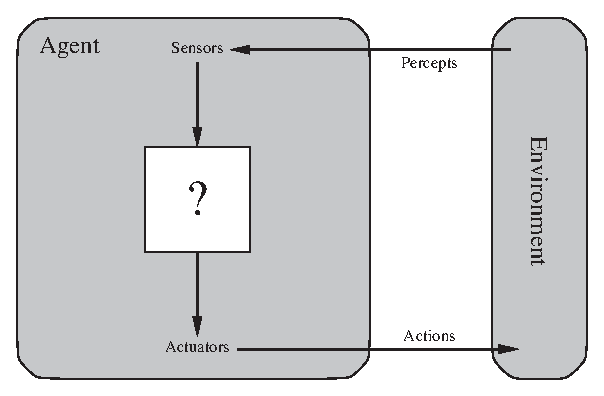
\includegraphics{Chapters/BackgroundKnowledgeAndRelatedWork/Figs/Vector/agent-environment.eps}
    \caption{Agent-Environment Interaction (Russell and Norvig)\cite[p.~35]{AIAMA}}
    \label{fig:agent_env_interaction}
\end{figure}
The box containing the question mark represents the agent's internal decision-making process, which generally speaking involves choosing an action, given the complete history of everything that the agent has perceived. The mapping from percept sequences to actions is described as the agent function. The agent function is an abstract notion; at a lower level an agent program implements the agent function, running on some physical system. A key concept in developing an agent program is rationality: "\textit{for each possible percept sequence, a rational agent should select an action that is expected to maximize its performance measure, given the evidence provided by the percept sequence and whatever built-in knowledge the agent has}"\cite[p.~37]{AIAMA}. This thesis is concerned with designing a system of agents that should exhibit rational behaviour.\newline
 

Russell and Norvig group agents into four common classes based on the design of the agent function\cite[p.~47]{AIAMA}: 
\begin{enumerate}
    \item \textbf{Simple reflex agents}: These agents select actions to take by ignoring the percept history to date, with the exception of the most recent percept.
    \item \textbf{Model-based reflex agents}: These agents have an internal state that depends on the percept history and is updated using new percepts. Updates occur using a model of the world.
    \item \textbf{Goal-based agents}: These agents are an extension to model-based reflex agents. They have some information about whether they have reached a "goal" state, which is desirable. The agent can choose actions to take based on the model. \note{Define what a goal state is.}
    \item \textbf{Utility-based agents}: A utility function is used as an internal performance measure in order to select actions. This allows an agent to pick among actions that may not immediately lead to a goal state.
\end{enumerate}
Recent work in the field of AI has strongly focused on learning agent architectures, which is a superset of all of the above agents. The key difference between the agent types listed above and a learning agent is that a learning agent has the ability to improve its performance through time independently. Its decision making process is not necessarily static and can change beyond its initial programming. An explanation of the architecture of a learning agent can be found in Russell and Norvig \cite[p.~55]{AIAMA}. Implementing each of these different types of agents requires varying degrees of effort. Depending on the problem, different architectures may be more or less suited, which suggests that fully understanding the problem that is attempted to be solved is of fundamental importance when designing an agent.

\subsection{Multi-Agent Systems}
Analogous to the definition of an agent, there is no universally agreed-upon definition of a \emph{Multi-Agent System} (MAS). A definition is provided in a field review paper by Stone and Veloso: "\textit{Multiagent Systems (MAS) is the subfield of AI that aims to provide both principles for construction of  complex  systems  involving  multiple  agents  and  mechanisms  for  coordination  of  independent  agents’ behaviors}" \cite{Stone2000MultiagentPerspective}. While the design of individual agents tends to focus on maximising a performance measure, the design of a multi-agent system is rather more multi-faceted. Weiss \cite{MAS:AModernApproachToDAI} notes that it is almost always oriented towards answering the question of "\textit{when and how to interact with whom}". Multi-agent systems have been proposed as a solution to many problems that modern AI attempts to tackle for some of the following reasons, which are outlined in more depth in \cite{Stone2000MultiagentPerspective}: 
\begin{itemize}
    \item Some problems by definition can be described as a multi-agent system. An example is an organization that may want to model it's internal affairs with a single system. The different departments have their own sub-systems that have differing priorities and capabilities; their interactions naturally can be thought of as interactions between independent agents, in accordance with the definition provided at the start of this section.
    \item The accomplishment of a task can be expedited significantly by using multiple agents. Multi-agents systems are part of the field of Distributed Artificial Intelligence (DAI) and so problem domains that decompose into several independent tasks that can be handled by separate agents can benefit from their use. The problem of efficient task allocation in multi-agent systems has been well-studied in the literature\cite{Gerkey2004ASystems}. 
    \item Robustness is an often-cited benefit of multi-agent systems. Distributed control means that failure of a single agent (mechanical or otherwise) may be tolerated.
    \item Multi-agent systems are often more scalable than single-agent systems. The necessary modularity of multi-agent systems means that adding new agents to the system can often be a solution to a more difficult problem, rather than adding new capabilities to a monolithic system. 
    \item The modularity of multi-agent systems means that the design and programming of them may be simplified. For example, rather than solving a multi-objective problem with a single agent, a single-objective problem may be solved with multiple agents. A result of this is that multiple cheap robots may be used to outperform a single, expensive robot \cite{Grabowski2000HeterogeneousExploration}.
\end{itemize}
\par



\section{Stochastic Target Localisation Related Literature}\label{sec:StochasticTargetLocalisationRelatedLiterature}



This section discusses the literature related to the problem of target localisation, pertaining to the first research question in Section \ref{sec:ResearchQuestions}. The necessary background knowledge to fully understand these approaches is provided in the next section (Section \ref{sec:StochasticTargetLocalizationBackground}).\par


We state problem of stochastic target localisation in a general setting as follows:
\\
\\
   \textit{ Given a region of space to explore and a set of heterogeneous autonomous aerial vehicles with sensing capabilities, devise a search strategy with a search cutoff criteria which will accurately return either the locations of the targets if one or more is present, or return that no targets are present, in the shortest possible time.}
\\
\\
\par The problem and its variants have been studied extensively and we survey the existing literature behind it here in chronological order. The study of problem can be traced back to a series of three papers by \citeauthor{KoopmanTheoryOfSearchTargetDetection} \cite{Koopman1956THEBASES}, \cite{KoopmanTheoryOfSearchTargetDetection}, \cite{Koopman1957TheEffort}. The first of the three, entitled "Kinematic Bases", references World War $\Romannum{2}$ as a primary motivation behind the series, citing "\textit{detection, location, and identification of targets}" as a key problem which required an urgent solution \cite{Koopman1956THEBASES}. Three key general features of search are identified, which are addressed individually in each of the three papers:
\begin{enumerate}
    \item "\textit{Kinematic Bases}" addresses search with a focus on the kinematic constraints involving the positions, geometric configurations and motion of the seachers and targets \cite{Koopman1956THEBASES}.

    \item "\textit{Target Detection}" is concerned with the stochastic nature of the sensors and instrumentation that is used when navigating and detecting \cite{KoopmanTheoryOfSearchTargetDetection}.
 
    \item "\textit{The Optimum Distribution of Searching Effort}" examines the probability of contact under the stated conditions. It also provides insight on how to optimise results by choosing a search strategy which maximises the probability of contact \cite{Koopman1957TheEffort}.
\end{enumerate}
\par This introduced the problem in structured manner and offered a strong insight into potential future research. In subsequent years the research branched into problems that involved the motion of both the searchers and the target \cite{Stone1980OptimalTargets}, or just the searchers \cite{Chew1966AProcedure}. Since the work in this thesis is primarily concerned with stationary targets, we refer the reader to the PhD. thesis \cite{Lau2007OptimalEnvironments} for a broad review of the literature related to search with a moving target. 

\citeauthor{Chew1966AProcedure} explored an instance of the search problem which is very close to the version this thesis explores \cite{Chew1966AProcedure}. The following assumptions were made
\begin{itemize}
    \item There is an object to be found in one of $R$ boxes at discrete locations or an $R+1^{st}$ representing the absence of the object.
    \item Sampling locations for the objects returns values with a false negative rate $\alpha_i$, which depends on the location.
    \item The boxes at discrete locations can be searched sequentially.
    \item All outcomes are independent, conditional on the location of the object and the search procedure used.
    \item A loss function introduces a cost for concluding the search when the object has not been found.
\end{itemize}
Note that no false positives were assumed to be observed. A dynamic programming approach was proposed, based on \cite{Blackwell1961DiscreteProgramming}, which was shown to be optimal when restricted to a fixed number of inspections. In this case, "optimal" is taken to mean that the strategy minimises the searcher's total expected cost of searching and stopping. A stopping rule was also suggested, with a proof of desirable properties such as minimizing expected cost when using an optimal search procedure.

\citeauthor{Black1965DiscretePROBLEM} examined a discrete instance of the stochastic target localisation problem for a stationary target, following the similar assumptions as \cite{Chew1966AProcedure} above, with the exception of the possibility of the object not being present (represented by the $R+1^{st}$ location) and without a cost for concluding the search when the object has not been found \cite{Black1965DiscretePROBLEM}. A sampling policy was proposed that was shown to be optimal in terms of minimising the expected cost of the search, according to an arbitrary cost function. The optimal policy was summarised as "\textit{Always look in the region for which the posterior probability (given the failure of earlier looks) of finding the object divided by the cost is maximum.}". The policy was not described in terms of a dynamic program, which the author claims provides more transparency to the solution, as opposed to previous work.

\citeauthor{Ross1969AStop} examined the search problem with the assumptions set out in \cite{Chew1966AProcedure} with the exception of the possibility of the object not being present (represented by the $R+1^{st}$ location) but did include the issue of when to conclude the search \cite{Ross1969AStop}. The paper showed that in general, an optimal search strategy exists for the problem with a penalty cost for stopping the search. He proved that when searching is warranted (i.e. the cost of stopping is small relative to the cost of further searching), the optimal search strategy is the same as in the no-penalty case. This means that to optimally solve the general problem of searching and stopping when a penalty cost for stopping is charged (as set out in \cite{Chew1966AProcedure}), the only additional requirement to the use of the optimal search strategy is a stopping time s* that is optimal when used with that search strategy.

\citeauthor{Chew1973OptimalProblem} then iterated on his previous work \cite{Chew1966AProcedure} and outlined a best stopping rule to accompany the optimal search procedure described in \cite{Chew1966AProcedure} with the work in \cite{Chew1973OptimalProblem}. This went a step further than \cite{Ross1969AStop}, since it included the possibility that the object is not present in the search region. The optimal stopping rule was found to be derived from the optimal dynamic programming strategy outlined in \cite{Chew1966AProcedure}, subject to a realistic technical condition relating the search termination cost, the cost of searching each location and the probability of a missed detection in each location.

\citeauthor{Kimeldorf1979BinomialObjects} studied the more general problem of locating $n$ objects hidden among $m$ boxes, where $m$ is known and $n$ is unknown \cite{Kimeldorf1979BinomialObjects}. They assume that there is a cost associated with searching each box and that the distributions of $p$ (the number of boxes) and $\pi$ (the distribution objects among the boxes) are known. They also assume that they know when all the objects have been found and that there is no associated search termination cost. Their results showed that for special cases of the distributions of $n$ and $p$, optimal search strategies can be found which are an extension of the general strategy set out in \cite{Blackwell1961DiscreteProgramming}.\par \citeauthor{Assaf1985OptimalApproach} tackled the same problem, but imposed the constraint that the distribution of $\pi$ is not known exactly, but instead some partial information is known about $\pi$ \cite{Assaf1985OptimalApproach}. Their findings showed that even small random fluctuations, or statistical inaccuracies, may give rise to results that are greatly different from the results obtained when $\pi$ is perfectly known. This suggested that a robust strategy in the case of a possibly inaccurate knowledge of $\pi$ would be desirable.

Many recent approaches related to the problem of non-deteministic detection and localisation of objects follow the groundwork laid by Elfes \cite{Elfes1989UsingNavigation}, whereby an \textit{occupancy grid} is used to represent the distribution of the target over the cells of a spatial lattice. Elfes describes an occupancy grid as a "\textit{probabilistic tesselated representation of spatial information}". In simpler terms, the occupancy grid is construc that can be used to maintain probabilities of occupation of cells that partition a region of space. % a tesselation of a physical space over which a mobile robot is intended to operate, with each cell maintaining a probability of the presence of an object. %This is in contrast to previous approaches that typically used geometric models of the world, which enforced strong domain-specific dependencies.
The approach was taken bearing in mind recent advancements in mobile robotics, with sensing and navigation abilities that allowed the processing of information from complex environments. There is an emphasis on designing the model to deal with an environment of which little may be known in advance, which is in contrast to previous approaches which assumed most aspects of the environment were known. The occupancy grids representation was defined to maintain an estimated environment state base on spatio-temporal data. A general Bayesian update rule is stated, which takes the current probabilities of cell occupation and updates them based on a new sensor reading: 
\begin{gather*}%\label{eq:OccUpdateRule}
%\centering
  \text{Probability of occupancy of grid cell } i \text{ given the set of observations } \{o_1, ..., o_{t+1}\} = \\
\frac{p(o_{t+1} | cell_i occupied) \times p(cell_i occupied | o_1, ..., o_t)}{\sum_{k=1}^{\# grid cells} p(o_{t+1} | cell_k occupied) \times p(cell_k occupied | o_1, ..., o_t)}
\end{gather*}
This allows the agent to maintain and recursively update the occupancy grid distribution based on new observations. This update rule is discussed in greater detail in Section \ref{section:HMMFiltering}. Elfes lists sonar based mapping and path planning as major applications of the occupancy grid framework.

%The book "\textit{Probabilistic Robotics}" \cite{Thrun:2005:ProbabilisticRobotics} was published with the goal of "\textit{providing a comprehensive introduction to the emerging field of probabilistic robotics}", which focuses on the techniques for processing percepts and designing control strategies, through statistical techniques. Many useful techniques are explored, and in particular there are two full chapters dedicated to the problem of localisation using mobile robots. We reference it often in the subsequent background section \ref{sec:StochasticTargetLocalizationBackground}.

A decentralized Bayesian approach to coordinating multiple autonomous mobile sensors, with the goal of localising a single stationary target, is presented in \cite{Bourgault2005DecentralizedSearch}. The approach is implemented using Bayesian Filtering, discussed in greater depth in this thesis in Section \ref{section:HMMFiltering}. Each autonomous airborne vehicle maintains its own probability density function (PDF) which is represented using an occupancy grid. Bayesian Distributed Data Fusion (DDF) is used to update each vehicle's individual PDF. The authors cite "\textit{scalability, modularity and adaptability}" as the motivation behind the approach. The results of running high-fidelity simulations for a target lost at sea using aerial vehicles demonstrated the feasibility of running the platform in real life.

In \cite{Chung2007ASearch}, Chung and Burdick proposed a general framework for the search problem, with a focus on the decision-making aspect of the agent implementing the search. An abstract sensor model was proposed, which assumed that observations are part of the set \{1,0\}, representing a positive and negative detection respectively. They introduced a sensor model which assumes a false positive rate ($\alpha$) and false negative rate ($\beta$) which can be calibrated before running the search. They also utilise an occupancy grid representation, with the corresponding Bayesian update rule updating the agent's belief based on new observations. They also described the use of Wald's Sequential Probability Ratio Test (SPRT) as a termination criteria for the search \cite{Wald1945SequentialHypotheses}. The mean time to decision (TTD) was reported for simulation runs which varied the search strategy for a single stationary target in a 10 $\times$ 10 grid, against which future results could be compared. Chung and Burdick extended this approach to multiple agents in \cite{Chung2008Multi-agentFramework}, finding that the best results were achieved using a hybrid search strategy (different search strategies were used for each agents, which had a complementary effect). Finally, \cite{Chung2012AnalysisStrategies} provides some theoretical analyses on special cases of their developed framework. Useful bounds are derived, including the minimum number of observations necessary to draw a conclusion.

\cite{Waharte2009CoordinatedUAVs}, \cite{Waharte2010ProbabilisticUAVs} and \cite{Waharte2010SupportingUAVsb} were published by authors working on the same project, named Sensing Unmanned Autonomous Aerial Vehicles (SUAAVE) \cite{Cameron2010SUAAVE:Details}. The work expands on the framework described by \citeauthor{Chung2007ASearch} in \cite{Chung2007ASearch}. Methods were proposed for dealing with observations that spanned multiple cells in the occupancy grid, motivated by the case that observations in the form of camera images do not always align with the grid. They also proposed the use of a feature-matching algorithm based on the SURF \cite{Bay2006SURF:Features} algorithm as a detection method based on aerial images. More search strategies were put forward and evaluated through the results of simulation, which demonstrated the effectiveness of a multi-vehicle approach.

%\cite{CollaborativeMultiRobotExploration} describes a system that is 

%Finally \cite{Kriheli2016OptimalInspections} gives a comprehensive overview of the history sequential discrete search. They discuss 



\section{Stochastic Target Localisation Background Knowledge}\label{sec:StochasticTargetLocalizationBackground}


%Should reference stone as well as koopman
First we present some of the tools that are used in the subsequent methodology chapters related to target localisation. \note{expand on this a bit more.}


\subsection{Hidden Markov Models}\label{subsec:BGHMM}
%\nomenclature[]{HMM}{Hidden Markov Model}
%\note{Add italics in places}
%\note{Could discuss:
%\\Background:
%What HMMs are,
%why they're useful in AI,
%the different commonly used HMMs. 
%\\ Use in my research:
%How the problem can naturally be described by a HMM,
%Lead into discussion of how DBN is a more natural way to describe the problem and how it leads to efficient factorization of densities for state estimation}
     
HMMs appear frequently in AI literature as they provide an abstract framework to deal with stochastic processes, which themselves are pervasive in their use as a tool to model real-world phenomena. This section will outline what HMMs are and their use in literature describing target localisation algorithms. A general overview of HMMs and Markov Processes can be found in \cite{Murphy1994DynamicLearning}, \cite{Ghahramani2001AnNetworks}, \cite{Bhattacharya2009StochasticApplications} and \cite{papoulis02}, on which we base the following discussion.

\subsubsection{Markov Processes}\label{subsubsec:MarkovProcesses}
It is instructive to understand what is meant by a stochastic process for some of the concepts mentioned in this thesis. A random process can be described as a family of random variables indexed by a set $\tau$: $\{X_t\}_{t\in\tau}$ \cite{Bhattacharya2009StochasticApplications}. Commonly in AI, stochastic processes model the evolution of a random system through \textit{discrete} time steps: $\tau$=$\mathbb N$. Examples of phenomena that are frequently modelled by stochastic processes include the growth of a bacterial population and the movement of a gas molecule \cite{Bhattacharya2009StochasticApplications}.\par

A first-order discrete-time Markov process is a stochastic process that describes a discrete-time stochastic process for which the first-order \textit{Markov property} holds \cite{Ghahramani2001AnNetworks}. The first-order Markov property states that the probability distribution of the n$_{th}$ random variable in the process is conditionally independent of all previous probability distributions in the sequence but the $n-1_{st}$: $P(X_t = x_t | X_{t-1} = x_{t-1}, X_{t-2} = x_{t-2}, ... , X_{1} = x_{1}) = P(X_t = x_t | X_{t-1} = x_{t-1})$ \cite{Ghahramani2001AnNetworks}. This is often referred to as the memoryless property of Markov processes. In order to describe a Markov process, it is therefore necessary to describe what is known as the transition function between each pair of timesteps: $P(X_t = x_t | X_{t-1} = x_{t-1})$. A common assumption is that the rules that govern state transitions are time invariant, meaning that they can be specified generally for any given pair of timesteps. This assumption will be made for the subsequent discussion. If $X_t$ is a discrete random variable defined over $S$ states, the transition function can be described by a stochastic matrix T, where T$_{i,j}$ = $P(X_t = j | X_{t-1} = i)$: 

\begin{center}
{$\displaystyle \left({\begin{matrix}T_{1,1}&T_{1,2}&\dots &T_{1,j}&\dots &T_{1,S}\\T_{2,1}&T_{2,2}&\dots &T_{2,j}&\dots &T_{2,S}\\\vdots &\vdots &\ddots &\vdots &\ddots &\vdots \\T_{i,1}&T_{i,2}&\dots &T_{i,j}&\dots &T_{i,S}\\\vdots &\vdots &\ddots &\vdots &\ddots &\vdots \\T_{S,1}&T_{S,2}&\dots &T_{S,j}&\dots &T_{S,S}\\\end{matrix}}\right)$}
\end{center}
\par

Some obvious results are worth pointing out; as for any stochastic matrix, by the axioms of probability theory, the sum of conditional probabilities across each column sum to one: {$\displaystyle \sum _{j=1}^{S}T_{i,j}=1$} and the transition probabilities over $k$ timesteps can be described by the $k_{th}$ power of the transition matrix: ${(T^k)}_{i,j}$ = $P(X_{t+k} = j | X_{t} = i)$. 
\begin{figure}[b!]
    \centering
    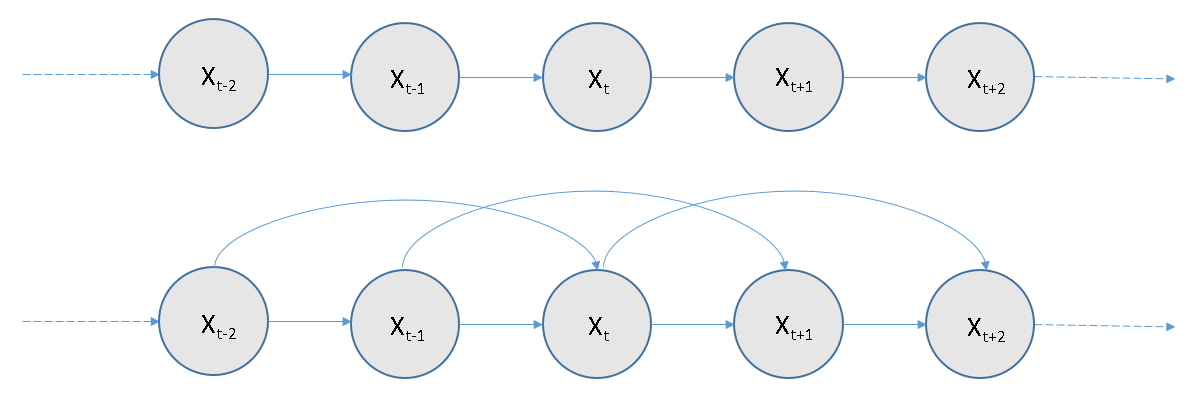
\includegraphics[width=0.8\linewidth]{Chapters/BackgroundKnowledgeAndRelatedWork/MultiAgentTargetDetectionBackground/Figs/MarkovProcesses/MarkovProcesses.png}
    \caption{A graphical model describing first and second order Markov processes}
    \label{fig:markov-processes}
\end{figure}
It also is possible to calculate the probability of the process experiencing a sequence of states from timesteps 1 as far as $t$, using the chain rule of probability and the Markov property:
$P(X_{1:t}) = P(X_1, X_2, ..., X_t) = P(X_1)\times P(X_2 | X_1)\times P(X_3 | X_2, X_1) \times P(X_t | X_{t-1}, X_{t-2}, ... , X_1) = P(X_1) \times \prod_{i=2}^{t}{P(X_i | x_{i-1})}$. Marginalization over variables in this sequence allows the calculation of many useful quantities.
\par

Markov processes can described by graphical models, for example Figure \ref{fig:markov-processes} displays a graphical representation of first and second order Markov processes, where a directed arrow between nodes represents a directional dependence between those nodes.

\subsubsection{HMM Description}\label{subsubsec:HMMDesc}
Hidden Markov Models (HMMs) are models that build on the Markov Process model, which describes the evolution of a random system in the language of probability theory. HMMs assume that the system being modeled can be described by a Markov process, but that the states of this process are unobservable \cite{Ghahramani2001AnNetworks}. This means that it is not possible to determine the state of the system exactly at any given point in time. However, it is possible to make an observation of a random variable that is related to the hidden state which yields information about the hidden state. A graphical representation of a HMM is shown in Figure \ref{fig:hmm}
\begin{figure}[]
    \centering
    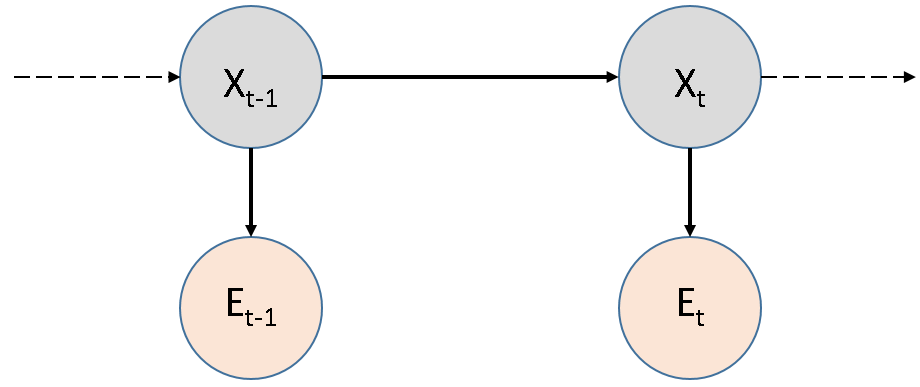
\includegraphics[width=0.8\linewidth]{Chapters/BackgroundKnowledgeAndRelatedWork/MultiAgentTargetDetectionBackground/Figs/HMMs/HMMGraphicalModel.png}
    \caption{A graphical model of a HMM}
    \label{fig:hmm}
\end{figure}
, where the Markov Process is shown by the variables $X_i$ and the observation variables are shown by variables $E_i$. A HMM can be specified by a triple, $\lambda$ = $(T, O, \pi)$, where $T$ is the stochastic transition matrix, $\pi$ is the initial distribution $P(X_1)$ and O describes the conditional probability of an observation given that the system is in a certain state: $O(E_i, X_i) = P(E_{i} | X_{i})$ \cite{Rabiner1989ARecognition}. Taken together, it is then possible to specify the joint distribution of the hidden state variables and the evidence variables, analogous to the Markov Process: 
$
P(X_{1:t}, E_{1:t}) = P(X_1, X_2, ..., X_t, E_1, E_2, ..., E_t) = P(X_1) \times P(E_1 | X_1) \times
\prod_{i=2}^{t}{(P(X_i | x_{i-1}) \times P(E_t | X_t))}.
$Given this representation, it is then possible to answer questions identified in \cite{Rabiner1989ARecognition} and \cite{Murphy1994DynamicLearning}:
\begin{itemize}

    \item Given the HMM, $\lambda$, determine the probability of occurrence of a particular observation sequence, $P(E_{1:t} | \lambda)$
    
    \item Given a sequence of observations $(E_1, E_2, ..., E_n)$, what is the most likely sequence of hidden states that led to these observations? i.e. find \[\argmax_{X_{1:t}} P(X_{1:t} | E_{1:t})\]
    
    \item Determine the parameters of $T$ and $O$, given a training set of observations, i.e. find the solution to \[\argmax_{\lambda} P(E_{1:t} | \lambda)\]
    
    \item \textit{Filtering}: What is the current distribution of the hidden state given all previous evidence ('belief state') of the agent at time t: $P(X_t | E_{1:t})$?
    
    \item \textit{Prediction}: What is the distribution of the hidden state in the future, given all evidence to date: $P(X_{t+k} | E_{1:t})$, for some k$>$0?
    
    \item \textit{Smoothing}: What is the distribution of a past state given all observations up to the current point in time: $P(X_k | E_{1:t})$, for some 0 $\leq$ k $<$ t?
    
\end{itemize}
\par

%Might include a subsection on a taxonomy of commonly used HMMs.

%\subsubsection{Summary}\label{subsubsec:Summary}
%In summary, HMMs can be used to abstractly describe the evolution of a stochastic system. They have been used to achieve state of the art performance in problems such as speech recognition \cite{ChiuSTATE-OF-THE-ARTMODELS} and ... . An comprehensive overview of extensions to the vanilla HMM can be found at \cite{Murphy1994DynamicLearning}.

\subsection{Dynamic Bayesian Networks}\label{subsec:BGDBN}


\begin{wrapfigure}{r}{0.7\textwidth}
    %\centering
    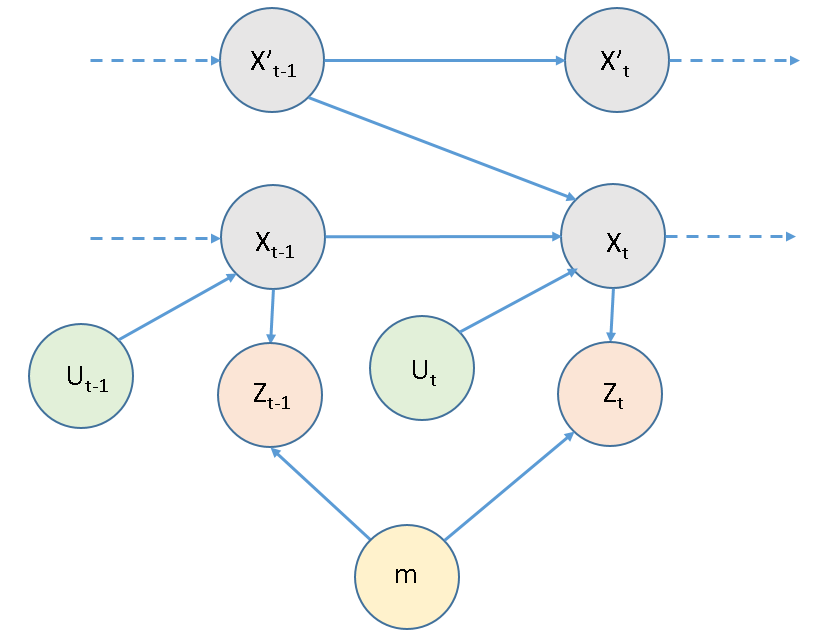
\includegraphics[width = 0.7\textwidth]{Chapters/BackgroundKnowledgeAndRelatedWork/MultiAgentTargetDetectionBackground/Figs/DBNs/Complex2TDBN.PNG}
    \caption{A DBN used for \textbf{S}imultaneous \textbf{L}ocalisation \textbf{a}nd \textbf{M}apping (SLAM), based on \cite[p.~311]{Thrun:2005:ProbabilisticRobotics}.}
    \label{fig:2TDBNExample}
\end{wrapfigure}

DBNs are a generalization of HMMs and are used to model time series. The key difference between DBNs and HMMs is that DBNs are not limited in how they decompose the hidden state variables of a complex stochastic system into the variables that represent its constituent conditional distributions \cite{AIAMA}. Rather than use a single random variable, $X_t$ to represent the state space, a set of random variables are used \cite{Murphy1994DynamicLearning}. DBNs can be considered as a special case of a Bayesian Network with an infinite number of nodes and repeating structure which specifies the transition probabilities between one time step and the next \cite[p.~204]{KollerPGM}. The hidden state variables are represented by nodes which have an associated conditional probability distribution (CPD) which states the probability of observing a value of a random variable given its parents: $p(X_i | Parents(X_i))$, where $i$ is the index of a node in the network \cite[p.~14]{Murphy1994DynamicLearning}. Given this representation, it is possible to calculate the joint distribution, $p(X_t | X_{t-1})$, of all $N$ state variables at time $t$ given the joint distribution at $t-1$ as \cite[p.~14]{Murphy1994DynamicLearning}:
\[
p(X_t | X_{t-1}) = \prod_{i=1}^{N}p(X_t^i | Parents(X_t^i)
\]
$i$ denotes the index of each $N$ variables in the network. \citeauthor{KollerPGM} provide a technical definition of DBNs: 
"\textit{A dynamic Bayesian network (DBN) is a pair $\langle B_0, B_\rightarrow \rangle$, where $B_0$ is a Bayesian network over $X^{(0)}$, representing the initial distribution over states, and $B_\rightarrow$ is a 2-TBN for the process. For any desired time span T $\geq$ 0, the distribution over $X^{(0:T)}$ is defined as a unrolled Bayesian network, where, for any $i$ = 1, . . . , $n$:
\begin{itemize}
    \item The structure and CPDs of $X^{(0)}_i$ are the same as those for $X_i$ in $B_0$,
    \item The structure and CPD of $X^{(t)}_i$ for $t > 0$ are the same as those for $X^{'}_i$ in $B_\rightarrow$.
\end{itemize}}" \cite[p.~204]{KollerPGM}. What this essentially means is that a DBN is a compact way of specifying an infinite set of Bayesian Networks (one for each $T>0$) with repeating structure.


Technically, every DBN can be represented as a HMM and visa versa, however, the number of parameters that need to be determined to represent DBNs can be significantly less than that of HMMs \cite{KollerPGM}. For example, consider the case of $n$ discrete random variables, each with support of size $m$. Specifying the full joint distribution without assuming any conditional independences between variables would require a number of probabilities exponential in the number of random variables, $m^{n}-1$, whereas specifying the same joint distribution as factored conditional distributions may require far fewer, reaching a number of probabilities directly proportional to the number of random variables, $n \times m$ in the degenerate case \cite[p.~63]{KollerPGM}. 
%\subsubsection{A Note on Bayesian Networks}
%A Bayesian Network (BN) is a graphical way to represent a particular factorization of a joint distribution. For a detailed explanation, the reader is referred to \cite{KollerPGM}. To fully explain a complex system, it is often natural to model it as the joint distribution of a number of random variables. This is in general intractable \cite{KollerPGM}. In order to circumvent this, independence properties in the distribution can be exploited to provide a much more compact representation of the distribution. BNs exploit the fact that independence is a strong notion that doesn't often occur in the real-world; however conditional independence is a weaker property that is far more prevalent, which still leads to the desired compact representation. BNs are described by a directed acyclic graph (DAG), $G$. The nodes in the graph correspond to the random variables whose joint distribution is of interest, and the arcs represent conditional independences. Specifically, if one Burglary points to Alarm as in figure \ref{fig:BayesianNetwork}, it is implied that the distribution of Alarm is conditionally independent on all other nodes in the network given Burglary. This means that only local conditional probability distributions must be provided in order to specify the full joint distribution.

%\begin{figure}
%example bayesian network figure
%\begin{tikzpicture}[
%  node distance=1cm and 0cm,
%  mynode/.style={draw,ellipse,text width=2cm,align=center}
%]
%\node[mynode] (i) {Burglary};
%\node[mynode,below right=of i] (g) {Alarm};
%\node[mynode,above right=of g] (c) {Earthquake};
%\path %(ra) edge[latex-] (sp)
%(g) edge[latex-] (c) 
%(g) edge[latex-] (i);
%\node[left=0.45cm of i]
%{
%\begin{tabular}{cM{3}M{3}}
%\toprule
%\multicolumn{2}{c}{Burglary} \\
%\multicolumn{1}{c}{T} & \multicolumn{1}{c}{F} \\
%\cmidrule(r){1-2}
%0.001 & 0.999 \\
%\bottomrule
%\end{tabular}
%};
%\node[right=0.45cm of c]
%{
%\begin{tabular}{cM{3}M{3}}
%\toprule
%\multicolumn{2}{c}{Earthquake} \\
%\multicolumn{1}{c}{T} & \multicolumn{1}{c}{F} \\
%\cmidrule(r){1-2}
%0.008 & 0.992 \\
%\bottomrule
%\end{tabular}
%};
%\node[below=0.5cm of g]
%{
%\begin{tabular}{ccM{2}M{2}}
%\toprule
%& & \multicolumn{2}{c}{Alarm} \\
%\multicolumn{2}{l}{Burglary Earthquake} & %\multicolumn{1}{c}{T} & \multicolumn{1}{c}{F} \\
%\cmidrule(r){1-2}\cmidrule(l){3-4}
%F & F & 0.01 & 0.99 \\
%F & T & 0.95 & 0.05 \\
%T & F & 0.8 & 0.2 \\
%T & T & 0.99 & 0.01 \\
%\bottomrule
%\end{tabular}
%};
%\end{tikzpicture}

%\caption{Simple Bayesian Network based on %\cite[P.~512]{AIAMA}}
%\label{fig:BayesianNetwork}
%\end{figure}



%\subsubsection{Dynamic Bayesian Network Technical Description}



%, which represent a general temporal probability model that describes a random system which is assumed to have a number of random variables, some of which are observable and some not \cite{AIAMA}.
%Dynamic Bayesian networks are usually used to represent the dynamics of a random system over time and can be described generally by specifying how the system transitions from its state at $t-1$ to $t$, if the first order Markov property is assumed. This thesis is concerned with the case when the first order Markov property holds. 
It is often convenient to categorise the random variables in the network into state variables (assumed to be hidden), control variables and observation variables \cite{Thrun:2005:ProbabilisticRobotics}. An example of a Dynamic Bayesian Network can be seen in Figure \ref{fig:2TDBNExample}. The hidden state variables are shaded in light grey, the observation variables in light orange and the control variables in light green. The directed arcs represent "instantaneous" causation, as with regular Bayesian Networks \cite[p.~15]{Murphy1994DynamicLearning}. Note that unlike HMMs, there isn't a requirement to have a single state and observation variable across each time-step and other variables can be introduced into the model.

%The nodes in the graph correspond to the random variables whose joint distribution we would like to calculate, and the arcs represent conditional independences \cite{KollerPGM}. Specifically, if one node points to another. \par













\subsection{Inference Algorithms}\label{subsec:BGInfAlgos}
%\nomenclature[]{MLE}{Maximum Likelihood Estimate}
%\note{Make sure it's clear whether using random variables or not}
%\note{Might need to make clear Markov assumptions }
As discussed, HMMs and DBNs are useful tools for modelling complex random dynamic processes. Typically, models are used to provide some kind of inference about a process, to gain insight into its inner workings. By inference, we mean calculating the probability distributions over variables of interest. Some algorithms will be outlined here that will demonstrate how to calculate both exact and approximate inferences, using general structures for HMMs and DBNs. \par

First, inference algorithms commonly used with HMMs are discussed, as their representation is more rigid, meaning that it is easier to exploit their structure generally to perform inference. As previously stated, HMMs and DBNs are routinely used to model systems that have state variables that cannot be directly observed. In most cases, we are interested in inferring what the state of the system might be, given the observed evidence variables received. This is the first and arguably the most useful inference challenge that we inspect.

The actual quantity that we want to compute is 
\[P(X_t | e_1, e_2, ..., e_t) = P(X_t | e_{1:t})\]
that is, the probability distribution of the hidden state variable, given all previously observed evidence variables. The notation $e_{1:t}$ denotes the joint distribution of $e_1, e_2, ..., e_t$. We are interested in computing this value, rather than the unconditional state distribution, $P(X_t)$, because we cannot observe the state directly, but we can observe the evidence variables. The conditional distribution $P(X_t | e_{1:t})$ is frequently referred to as the \textit{belief state} and the process of calculation of this distribution is frequently referred to as \textit{state estimation} or \textit{filtering} \cite{AIAMA}, \cite{Thrun:2005:ProbabilisticRobotics}, \cite{KollerPGM}. The \textit{forward algorithm} can be used to calculate the value of $P(X_t | e_{1:t})$ \cite[p.~572]{AIAMA}. It is a recursive algorithm, and takes advantage of the fact that the underlying process is Markovian. The forward algorithm for HMMs is shown in Algorithm \ref{alg:forwardAlgorithmHMMs} and is based on the algorithm outlined in \cite[p.~27]{Thrun:2005:ProbabilisticRobotics}. The derivation is useful to follow as an exercise, so we present it in the subsequent sub-section.
\subsubsection{HMM Filtering Algorithm Derivation} 
\label{section:HMMFiltering}
\note{Might be better to put this in an appendix.}
Two well-known probability identities are used in the derivation: 
\note{Fix the formatting here}
\begin{center}
%- - - - - - - - - - - - - - - - - - - - - - - - - - - - - - - - - - - - - - - - - - - - - - - - - - - - - - - - - - - - - 
\end{center}
%quad adds space
\[(a) \quad p(A | B, C) = \frac{p(B | A, C) p(A | C)}{p(B | C)} \quad \text{and} \quad (b) \quad p(A | B) = \int\limits_{C}P(A | B, C) P(C | B)dC\]

\begin{center}
%- - - - - - - - - - - - - - - - - - - - - - - - - - - - - - - - - - - - - - - - - - - - - - - - - - - - - - - - - - - - - 
\end{center}
The derivation is as follows:
\begin{enumerate}
\item {$ p(X_t | e_{1:t}) = p(X_t | e_{1:t-1}, e_t) $ }

\item{$ \text{applying (a) and letting} \quad \eta = \frac{1}{p(e_t | e_{1:t-1})} \quad = \quad \eta p(e_t | e_{1:t-1}, X_t)p(X_t|e_{1:t-1}) $ }

\item{$ \text{by the Markov property} \quad = \quad \eta p(e_t | X_t)p(X_t|e_{1:t-1})$}

\item{$\text{applying (b)} \quad =  \quad \eta p(e_t | X_t)\int_{X_{t-1}}p(X_t|e_{1:t-1}, X_{t-1}) p(X_{t-1}|e_{1:t-1})dX_{t-1}$}

\item{$ \text{by the Markov property} \quad = \quad \eta p(e_t | x_t)\int_{X_{t-1}}p(X_t|X_{t-1}) p(X_{t-1}|e_{1:t-1})dX_{t-1} $}

\end{enumerate}
Note that $\eta$ is a normalizing constant that ensures that the probability distribution integrates to 1, and that the probabilities that need to be calculated can be done so from the parameters specified in the HMM; namely $p(e_t | X_t)$, specified by the sensor model, and $p(X_t | x_{t-1})$, specified by the transition model.

\begin{algorithm}{}
\caption{Forward Algorithm for HMMs}
\label{alg:forwardAlgorithmHMMs}

\begin{algorithmic}[1]
\renewcommand{\algorithmicrequire}{\textbf{Input:}}
\renewcommand{\algorithmicensure}{\textbf{Output:}}
%Input
\REQUIRE $\newline P(x_{t-1} | e_{1:t-1})=bel(x_{t-1}): \quad \text{The belief distribution as far as the previous time-step}
\newline e_t: \quad \text{The most recent observation}
\newline hmm: \quad \text{A Hidden Markov Model specifying the transition and observation probabilities,} \newline p(X_t | x_{t-1}) \text{ and } p(E_t | x_t)$
%Output
\ENSURE  $\newline P(X_{t} | e_{1:t}) = bel(X_{t})$

\hfill\pagebreak

\FOR{all $x_t$}
\STATE $\overline{bel}(x_t) = \int p(x_t | x_{t-1}) p(x_{t-1} | e_{1:t-1}) d x_{t-1}$
\STATE $bel(x_t) = p(e_t | x_t) \overline{bel}(x_t)$
\ENDFOR
\STATE $ \eta = 1 / \int_{x_t}{bel(x_t)}dx_t$
 \FOR{all $x_t$ do:}
\STATE $bel(x_t) = \eta{bel}(x_t)$
\ENDFOR  
    
%\ENDWHILE
\RETURN $bel(X_t)$
\end{algorithmic} 
\end{algorithm}

\note{Don't forget to mention: Sufficient statistics, forward algorithm}

Algorithm \ref{alg:forwardAlgorithmHMMs} uses integrals to account for the fact that the distribution of the hidden state, $X_t$, may be continuous. The work done in this thesis only uses discrete distributions, and so summations are used instead of integrals for the subsequent discussion. A consequence of using discrete distributions is that it is possible to formulate the forward algorithm using vector and matrix notation. As outlined in Section \ref{subsec:BGHMM}, the transition model $T=p(X_t | X_{t-1})$ for a HMM can be written down in matrix form, as can the observation model $O_t=p(E_t | X_T)$. This allows for a highly compact notation: denoting $p(x_t | e_{1:t})$ as $f_{1:t}$, we can write $f_{1:t} = \eta O_{t} T^{T} f_{1:t-1}$, where $f_{1:t}$ contains the vector of values of $p(x_t | e_{1:t})$ for every possible $x_t$ \cite[p.~579]{AIAMA}. Note that the observation model, $O_t$ is time dependent, as opposed to the transition model, which is assumed to be stationary. \par

Some insight can be gained from studying Algorithm \ref{alg:forwardAlgorithmHMMs}. There are three main steps to this algorithm, and the intuition behind them is explained based on explanations in \cite{AIAMA}, \cite{Thrun:2005:ProbabilisticRobotics} and \cite{Murphy1994DynamicLearning}: 
\note{These are highly verbose, edit to make less wordy}
\begin{enumerate}
    
    \item The first step is often referred to as the prediction step:
    \begin{center}
    $\overline{bel}(x_t) = \sum_{x_{t-1}} p(x_t | x_{t-1}) p(x_{t-1} | e_{1:t-1}) d x_{t-1}$
    \end{center}

    This step carries out the first part of the calculation of the belief value for a given state $x_t$, by marginalizing over all possible hidden states ($x_{t-1}$) that could have preceded the current one ($x_t$). This reflects intuition: the probability of being in state $x_t$ should depend on the probability of transitioning from all possible previous states to $x_t$. 
    %\note{this sentence doesn't seem necessary}
    Think "\textit{the probability that I am in location x is the sum of probabilities of starting at all other possible locations and subsequently ending up in location x, weighted against my belief that I began in each other possible location}".
    
    %product of our most recent belief of being in state $x_{t-1}$, given by $p(x_{t-1} | e_{1:t-1})$ and the probability of transitioning from that state to state $x_{t}$, for all previous possible states that we could have been in. 
    $\overline{bel}(x_t)$ effectively projects our current belief to the next time step by using the transition probabilities specified in the HMM.
    
    \item The second step is often referred to as the correction step, or the measurement update step: 
    \begin{center}
    $bel(x_t) = p(e_t | x_t) \overline{bel}(x_t)$ 
    \end{center}
    This step takes the projected belief in step 1 and multiplies it by the probability of observing the data that we did in the given hidden state, $x_t$. This can be thought of as a correction because the use of the measurement data narrows the probabilities of the possible states that the system could have transitioned to. 
    \note{Need to re-word this to make more concise}
    %For example, if the value of a transition probability from state x to state y is low, and there is a low probability that the system was previously in state x, a high probability of observing the observed sensor reading given state y can still result in a relatively high posterior probability of the system being in state y given the new evidence.
    
    \item The final step is to ensure that the distribution sums to 1. This is done by multiplying by a normalizing constant, $\eta$.
    
    
\end{enumerate}
A key strength of this algorithm is the fact it allows updates to be performed online. The reason for this is that the information-state vector, $p(x_t | e_{1:t})$ is a sufficient statistic for the past history of observations. For a full proof of this property, the reader is referred to Appendix A of \cite{Smallwood1973TheHorizon}, which also provides insight into the update rule itself. In relation to the update rule, note that an initial distribution of the estimated state must be provided to this algorithm before the first update can be performed. The complexity of the forward algorithm is $\theta (nm^2)$, where m is the size of the joint distribution of the hidden variables, x, and n is the number of time-steps that have occurred. This is clear to see when viewing the update as the matrix-vector multiplication $f_{1:t} = \eta O_{t} T^{T} f_{1:t-1}$, as the size of T is $m^2$.






\subsubsection{Evidence Likelihood Algorithm Using a HMM}\label{subsubsec:EvLikelihood}
\note{Will talk about this briefly for SPRT}
The second useful quantity that we would like to calculate is the probability of observing the evidence that we did, often referred to the likelihood function of the data, as identified in Section \ref{subsec:BGHMM}. In simpler terms, this is the calculation of the probability of observing the data, given a fixed parameterised model of the data (the HMM). This value is useful as it can reveal insights into whether one model is more likely than another model, with applications including \textbf{M}aximum \textbf{a} \textbf{P}osteriori (MAP) parameter estimates and hypothesis testing. It is used in this thesis in Section \ref{subsubsec:SeachTerminationMethodology}. We would like to compute the value of
\[P(e_1, e_2, ..., e_t) = P(e_{1:t})\]
given the fixed set of parameters provided by the HMM. A brief outline of the derivation is shown:\note{might be best to put the derivation in an appendix} 


\subsubsection{HMM Evidence Likelihood Algorithm Derivation}\label{subsubsec:BGEvidenceLikelihood}

Analogous to the filtering algorithm derivation, two well-known probability identities are used in the derivation: 
\begin{center}
%- - - - - - - - - - - - - - - - - - - - - - - - - - - - - - - - - - - - - - - - - - - - - - - - - - - - - - - - - - - - - 
\end{center}
%quad adds space
\[(a) \quad p(A, B, C) = p(A | B, C) p(B, C) \quad \text{and} \quad (b) \quad p(A, B) = \sum_{C}{p(A | B, C)p(B, C)}\]

\begin{center}
%- - - - - - - - - - - - - - - - - - - - - - - - - - - - - - - - - - - - - - - - - - - - - - - - - - - - - - - - - - - - - 
\end{center}

The derivation is as follows:
\begin{enumerate}

\item {$p(e_{1:t}) = \sum_{x_t}p(e_{1:t}, x_t) \quad = \quad \sum_{x_t}p({e_{1:t-1}, e_t, x_t}) $
}
\item {$\text{applying (a) } \quad= \quad
\sum_{x_t}{p(e_t | e_{1:t-1}, x_t)p(x_t, e_{1:t-1})}$
}
\item{$\text{by the Markov property} 
\quad = \quad \sum_{x_t}p(e_t | x_t)p(x_t, e_{1:t-1})$
}

\item{$\text{applying (b)} \quad =  \quad
\sum_{x_t}p(e_t | x_t) \sum_{x_{t-1}}p(x_t|e_{1:t-1}, x_{t-1}) p(x_{t-1},e_{1:t-1})$
}

\item{$\text{by the Markov property} \quad = \quad 
\sum_{x_t}{p(e_t | x_t)\sum_{x_{t-1}}p(x_t|x_{t-1}) p(x_{t-1},e_{1:t-1})}$
}

\end{enumerate}

The algorithm for calculating likelihoods uses the forward algorithm, $\alpha$, with the replacement of  $p(x_{t-1}|e_{1:t-1})$ with $p(x_{t-1}, e_{1:t-1})$ and one final summation. This means that it is possible to use the forward algorithm to calculate likelihoods: $p(e_{1:t}) = \sum_{i=1}^{n} \alpha(x_i, e_i)$, where $\alpha(x, e)$ is the result of applying the forward algorithm to the sequence of evidence variables $(e_1, ..., e_t)$.


%No point in writing up likelihood algorithm as it's very similar to forward algorithm.

%\subsubsection{HMM Parameter Learning Using Expectation Maximization}\label{subsubsec:EMAlgo}
%\note{Can talk about this briefly for battery model}
%Since a HMM is a parameterised model of a stochastic process, a natural question to ask is whether it is possible to determine a \textit{"best"} set of parameters to describe the process, by using observations of the process. This is a more complex version of the well-known process of finding the parameters that maximize the likelihood function of fully observable data, known as the \textbf{M}aximum \textbf{L}ikelihood \textbf{E}stimate (MLE). Finding the most likely set of parameters which provided the observed values can be described mathematically as the value of \note{fix argmax notation}$\argmax_{\lambda} P(E_{1:t} | \lambda)$. Note that this is a fundamentally different problem to that discussed in the preceding section; here we do not assume a fixed set of parameters for the HMM ($\lambda$).

%This is a well-studied problem for HMMs and the solution is given by the \textbf{E}xpectation \textbf{M}aximisation (EM) algorithm, proposed by \citeauthor{Dempster1977MaximumAlgorithm}. This algorithm is reasonably complex and highly detailed overviews can be found in many texts that deal with parameter estimation for statistical models. A quick outline of how the algorithm works is provided here.\par


%The reason why the standard methods for finding the MLE for a parameterised model do not work with HMMs is due to the fact that there is no way to directly express the quantity  $P(E_{1:t} | \lambda)$ directly. This can be seen in the derivation of the evidence likelihood in <reference whichever appendix it ends up in>. Instead, it is necessary to marginalize over states: $ P(e_{1:t} | \lambda) = \sum_{x_t}{p(x_t, e_{e:t} | \lambda)}$. The standard approach to finding the parameters that maximize a model is to take a log transform of the likelihood function, which preserves the solution but turns the problem into one of finding the parameters that maximize a sum rather than a product. Using standard methods of calculus, this can usually be done easily. The issue with HMMs is that when a logarithmic transformation is applied to the likelihood function, the summation sign remains within the log function, which means finding the maximum is still a difficult problem. The EM algorithm, taking the approach of many iterative techniques, relaxes the constraints on the problem in order to find a lower bound of the log-likelihood and then iteratively improves this lower bound with increasing likelihood values. 


%The Baum-Welch algorithm is a special case of the EM algorithm and is frequently used to solve the problem of estimating the parameters of a HMM. The algorithm is described fully in appendix <reference appendix>.


\subsubsection{Filtering Algorithm for DBNs}\label{subsubsec:filteringDBN}
\note{Extend HMM to add control variable}
\begin{wrapfigure}{r}{0.68\textwidth}
    \centering
    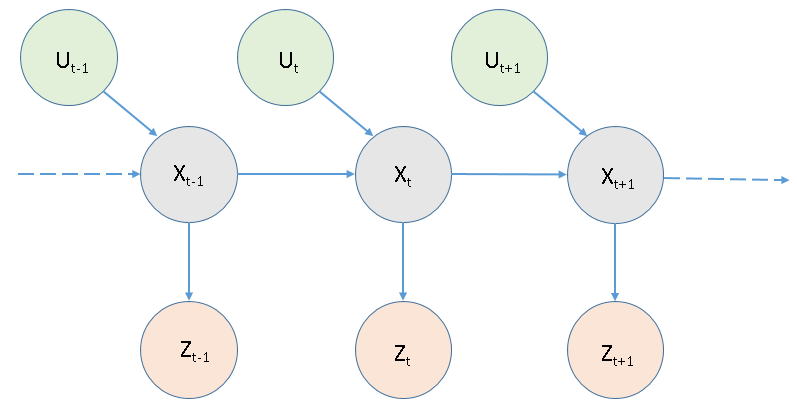
\includegraphics[width = 0.68\textwidth]{Chapters/BackgroundKnowledgeAndRelatedWork/MultiAgentTargetDetectionBackground/Figs/HMMs/HMMWithControl.png}
    \caption{A DBN with Hidden State variables (grey), Observation variables (orange) and Control variables (green).}
    \label{fig:HMMWithControlVariablesExample}
\end{wrapfigure}
The forward algorithm for state estimation was presented in Section \ref{section:HMMFiltering}. A slightly modified version of this algorithm is now described, which is very commonly used in stochastic systems that can be influenced by actions that an agent may take. Such systems have \textit{control variables} as well as hidden state variables and observation variables. These control variables (variables which represent the actions that an agent may perform) have an influence on the transition probabilities between states. The graphical model in Figure \ref{fig:HMMWithControlVariablesExample} describes the basic case. The arrows describe the conditional independence assumptions: at time t, the hidden state ($x_t$) depends on the previous state ($x_{t-1}$), and the previous control action taken ($u_t$). As with the HMM, the observation $e_t$ is conditionally dependent on the state $x_t$. This causes a slight change in the filtering algorithm: on line 2 of algorithm \ref{alg:forwardAlgorithmHMMs}: $\overline{bel}(x_t) = \sum_{x_{t-1}} p(x_t | x_{t-1}) p(x_{t-1} | e_{1:t-1}) $ is replaced with $\overline{bel}(x_t) = \sum_{x_{t-1}} p(x_t | u_t, x_{t-1}) p(x_{t-1} | e_{1:t-1}, u_{1:t-1})$, reflecting that transition probabilities now depend on the most recent control action taken, as well as the previous state.


%DBNs have already been shown to be a powerful tool while modelling stochastic systems, since the hidden variables can be described by conditional independences, rather than 



%This algorithm can be further generalized - if multiple control variables, hidden state variables and observation variables are needed to describe the system fully, it is possible to make minor modifications which reflect the conditional independences stated by the underlying DBN by .

It is worth noting that there are many filtering algorithms that deal with data that come from certain distributions and satisfy constraints related to their transition and observation models, for example the Kalman Filter \cite[p.~43]{Thrun:2005:ProbabilisticRobotics}.






%\subsubsection{Discrete Bayes Filter}
%\note{This is what is used in the work that I did, so it is outlined}

\subsubsection{Approximate State Estimation}
\note{Thought about using Particle filter to avoid the dimensionality problem when attempting to maintain estimated state}
The state estimation algorithms mentioned so far maintain the exact values of the distribution $p(x_t | e_{1:t}, u_{1:t})$, but we will quickly mention an approximate method that is also frequently used. The computational complexity of the filtering algorithms is determined by how well the joint distribution of hidden state variables, observation variables and control action variables can be factored, but in the worst case the complexity is given by the case where the joint distribution of the hidden state variables cannot be factored at all. The forward algorithm, described in Algorithm \ref{alg:forwardAlgorithmHMMs} for a HMM performs the update from each time state in O($n^2$), where $n$ is the dimension of the hidden state variable \cite{Smyth1997ProbabilisticModels}.
%$O(n^2ut)$, where n are the number of hidden states, u is the number of available control actions and t is the number of time steps.
In some cases, this can become intractable if the state space is large enough. % and the transition model cannot be factored. 
In this case, approximate techniques are used. An example is the \textit{particle filter}. Details of the particle filter can be found in \cite[p.~96]{Thrun:2005:ProbabilisticRobotics} and \cite[p.~665]{KollerPGM}.


\subsection{Prediction Algorithms}
\placeholder{}
This contains the details of prediction algorithms

\subsection{Sequential Statistical Hypothesis Testing}\label{subsec:SPRT}
%outlines the background behind the sequential probability ratio test.

\note{This section assumes that the reader has a basic familiarity with the terminology and techniques of hypothesis testing in statistics.}

A statistical test is a mechanism for making quantitative decisions about a process, by determining how well the data stand in agreement with given predicted probabilities \cite{cowan1998statistical}. Statistical tests are usually used to draw conclusions about a \textit{statistical hypothesis}, which is a testable hypothesis based on observations of a process that is modelled using random variables. There are many texts that outline the statistical tests that can be used to make a decision between accepting and rejecting the null hypothesis, $H_0$, for example \cite{IntroductionToMathematicalStatistics}. The usual context in which this occurs is one in which the data has been collected in advance and the sample size is fixed and known. The standard procedure for testing a simple hypothesis involves using a Uniformly Most Powerful (UMP) Test for a fixed value of the probability of making a Type \Romannum{1} error, $\alpha$ \cite[p.~253]{IntroductionToMathematicalStatistics}. The subsequent sections discuss how this can be extended to a sequential paradigm, where the sample size is not fixed.\note{An example might be of value here} \par

There exists a branch of statistical hypothesis testing called \textit{sequential hypothesis testing}, which is used when the sample size is not fixed in advance \cite[p.~375]{IntroductionToMathematicalStatistics}. Given a hypothesis to test, $H_0$, this means the decision process goes beyond deciding whether to accept or reject the null hypothesis, but to either
\begin{enumerate}
    \item Accept the hypothesis being tested, $H_0$.
    \item Reject the hypothesis being tested, $H_0$
    \item Continue the experiment by making a further observation.
\end{enumerate}

It is clear that samples are gathered as long as 1). or 2). above are not chosen, which intuitively corresponds to the notion of making an informed decision, where it is desirable to ensure that enough data has been gathered to draw a meaningful conclusion. In the sequential testing paradigm, two kinds of error may be committed, as with the non-sequential case: we may reject the null hypothesis when it is true (commit a Type \Romannum{1} error) or we may accept the null hypothesis when some alternative hypothesis is true (commit a Type \Romannum{2} error). 

The Sequential Probability Ratio Test (SPRT), which was devised by \citeauthor{Wald1945SequentialHypotheses}, proposes a statistical test for simple hypotheses with specified fixed values, which ensures that the probability of Type \Romannum{1} and Type \Romannum{2} errors do not exceed $\alpha$ and $\beta$ respectively \cite{Wald1945SequentialHypotheses}. \citeauthor{Wald1948OptimumTest} proved that the SPRT is optimal, in the sense that of all tests with the same power, the SPRT requires on average the fewest number of observations to reach a decision \cite{Wald1948OptimumTest}. A strong advantage of the test is that it can be carried out without determining any probability distributions whatsoever \cite{Wald1945SequentialHypotheses}. The SPRT can be thought of as a stopping rule for sampling in a stochastic process. For the sake of brevity, we omit the full derivation of the rule and the proof of optimality, but instead refer the reader to \cite{Wald1945SequentialHypotheses}, \cite{Wald1950BayesProblems} and \cite{Wald1948OptimumTest}. The SPRT can be carried out following the procedure shown in Algorithm \ref{alg:SPRT}.


%\begin{enumerate}
%    \item The null and alternative hypotheses are stated, $H_0$ and $H_1$.
%    \item The desired type \Romannum{1} and type \Romannum{2} error rates are specified as $\alpha$ and $\beta$.
%    \item Calculate the values $A = \frac{1-\beta}{\alpha}$ and $B = \frac{\beta}{1-\alpha}$
%    \item 
%\end{enumerate}


\begin{algorithm}{}
\caption{The Sequential Probability Ratio Test Algorithm}
\label{alg:SPRT}

\begin{algorithmic}[1]
\renewcommand{\algorithmicrequire}{\textbf{Input:}}
\renewcommand{\algorithmicensure}{\textbf{Output:}}
%Input
\REQUIRE $\newline \alpha \text{: \quad The upper limit in probability for making a type \Romannum{1} error.}$
\newline $\beta \text{: \quad The upper limit in probability for making a type \Romannum{2} error.}$
\newline $H_0 \text{: \quad The null hypothesis.}$
\newline $H_1 \text{: \quad The alternative hypothesis.}$
\newline $(x_1, ..., x_m) \text{: \quad The m observations made so far.}$
%Output
\ENSURE  $\newline$ A decision to accept $H_0$, accept $H_1$ or make another observation.\\
\hfill\pagebreak

\STATE Calculate $p_{0m}=p_{0m}(x_1, ..., x_m)$, the probability of observing the data under the assumption $H_0$ is true.

\STATE Calculate $p_{1m}=p_{1m}(x_1, ..., x_m)$, the probability of observing the data under the assumption $H_1$ is true.

\STATE Calculate the values $A = \frac{1-\beta}{\alpha}$ and $B = \frac{\beta}{1-\alpha}$

\STATE Accept $H_1$ if $\frac{p_{1m}}{p_0m} \geq A$

\STATE Accept $H_0$ if $\frac{p_{1m}}{p_0m} \leq B$

\STATE Make an additional observation if $B < \frac{p_{1m}}{p_0m} < A$



\end{algorithmic}
\end{algorithm}


The main idea, as is the case with simple non-sequential hypothesis tests, is based on the idea that if the likelihood ratio ($\frac{p_{1m}}{p_{0m}}$) lies in some \textit{critical region}, $C$, then we may reject the null hypothesis \cite{IntroductionToMathematicalStatistics}. The SPRT extends this by partitioning the m-dimensional sample space $M_m$ into three mutually exclusive regions, $R_m^0$, $R_m^1$ and $R_m$. After the $i_{th}$ observation $(x_i)$ has been drawn, $H_0$ is accepted if $(x_1, ..., x_i)$ lies in $R_m^0$, $H_1$ will be accepted if $(x_1, ..., x_i)$ lies in $R_m^1$ or a $i+1_{th}$ observation will be drawn if $(x_1, ..., x_i)$ lies in $R_m$ \cite{Wald1945SequentialHypotheses}. The process of how to choose $R_m^0$, $R_m^1$ and $R_m$ is outlined in Section 3 of \cite{Wald1945SequentialHypotheses}, which goes beyond the scope of this thesis. The derivation essentially shows that $(x_1, ..., x_i) \in R_m^0$ is equivalent to $\frac{p_{1m}}{p_0m} \leq B$, $(x_1, ..., x_i) \in R_m^1$ is equivalent to $\frac{p_{1m}}{p_0m} \geq A$, and $(x_1, ..., x_i) \in R_m$ is equivalent to $B < \frac{p_{1m}}{p_0m} < A$.

\subsubsection{Summary}
The SPRT is a sequential hypothesis test that formulates a stopping rule in order to draw conclusions based on statistical data. It has frequently been in quality control studies, where samples can be expensive to gather, but it can be applied in other scenarios where sampling can be expensive \cite{Ou2010AnMean}. We use it in Section \ref{subsubsec:SeachTerminationMethodology}

\subsection{Related Literature}
\workinprogress

A problem explored in this thesis is an instance of target detection using a system of aerial robots. A more primitive version of this problem initially gained traction in the literature with the work of Koopman \cite{KoopmanTheoryOfSearchTargetDetection} and has received much attention since. More recent papers have framed the problem in terms of agents and multi-agent system. %Citations needed
A common feature in the problem definition in the literature is that the system of agents are assumed to work in a partially observable environment\cite{Symington2010ProbabilisticUAVs}, \cite{Chung2008Multi-agentFramework}, \cite{WongMulti-vehicleTargets}. Many recent approaches follow the groundwork laid by Elfes\cite{ElfesUsingNavigation}, whereby an "occupancy field" is used to represent the distribution of the target over the cells of a spatial lattice. Elfes describes an Occupancy grid as a "probabilistic tesselated representation of spatial information". This is in contrast to previous approaches that typically used geometric models of the world, which enforced strong domain-specific dependencies. The occupancy field framework 
\par

\section{High Fidelity Simulation Environments}
In this section, we discuss existing literature and common approaches related to designing and implementing high-fidelity simulation environments. This provides a backdrop for Chapter \ref{chap:HighFidelitySim}, which describes the work we did to implement our own custom high-fidelity simulation environment.
\subsection{High Fidelity Simulation Environments Related Literature}\label{sec:SimulationEnvironmentsRelatedLiterature}
%Want to introduce the problem to allow for a discussion that makes sense. Ideally will frame a problem so that it suggests that having a high-fidelity simulation environment would be very useful for the project and in general.
%\nomenclature[]{UUV}{Unmanned Underwater Vehicle}
\subsection{Key Aspects of Simulation Environments}
We begin by discussing some key aspects of simulation environments that serve as a starting point on which more advanced techniques build upon. According to %\citeauthor{Shannon1998INTRODUCTIONSIMULATION} 
\citeauthor{Shannon1998INTRODUCTIONSIMULATION}, simulation can be defined as \textit{"the process of designing a model of a real system and conducting experiments with this model for the purpose of understanding the behavior of the system and/or evaluating various strategies for the operation of the system"} \cite{Shannon1998INTRODUCTIONSIMULATION}. Simulations have been used extensively to model complex systems since the invention of the modern computer, gaining traction since the proposal of the Markov Chain Monte Carlo method by Stansislaw Ulam and John Von Neumann in the late 1940s \cite{Robert2011AIncomplete}. Simulations written with software are created in order to gain insight into the system's dynamics and to evaluate results of using a method intended for real-world use. This is usually because proposed methods may be too time-consuming or expensive to test in the real world. Software simulations are being used increasingly for a wide variety of tasks, from planning new roads to alleviate traffic \cite{Pell2017TrendsSimulation} to developing self-driving vehicles \cite{Dosovitskiy2017CARLA:Simulator}. 

Designing simulations allows the developer of an agent-based system to abstract away details of the real-world conditions that the agents will act in and focus on the salient aspects that the agents are concerned with, in order to prototype, train, test, analyse and validate. General advantages of simulations are listed in  \cite{Shannon1998INTRODUCTIONSIMULATION}, with the most notable being:
\begin{itemize}
    \item \textit{"It can be used to explore operating procedures, decision rules, organizational structures, etc. without disrupting the ongoing operations."}
    \item \textit{"Simulation allows us to control time. Thus we can operate the system for several months or years of experience in a matter of seconds allowing us to quickly look at long time horizons or we can slow down phenomena for study."}
    \item \textit{"It allows us to gain insights into how a modelled system actually works and understanding of which variables are most important to performance."}
    \item \textit{"Simulation's great strength is its ability to let us experiment with new and unfamiliar situations and to answer "what if" questions."}
\end{itemize}


\note{Following paragraph doesn't really belong here but does help tie everything together}

 In relation to designing intelligent agents, often the trade-off between exploration and exploitation is referenced. Exploration or "information gathering" \cite{AIAMA} can be considered as the agent posing a "what if" question in order to learn the consequences of performing action, and exploitation can be considered as an agent using gathered or previous knowledge to choose actions to take that maximize its performance measure, as outlined in Section \ref{AgencySubsection}. Since simulation environments are highly suited to answering "what if" questions, which has motivated the use of using simulations to design systems of autonomous agents in the literature, for example the simulation environment used in the 
\href{https://multiagentcontest.org/}{Multi-Agent Programming Contest.}\footnote{\href {https://multiagentcontest.org/}{https://multiagentcontest.org/}}



\subsection{Simulation Environments Design Using Game Engines}\label{subsec:GameEngineReview}
Since computer games are effectively simulations, the technologies used to create them have also been used to create simulations for a more serious purpose, often referred to in the literature as \textit{serious games}. Serious games usually refer to games that have been specifically designed to provide training to professionals working in an industry where extensive training is necessary but difficult, expensive or dangerous to provide \cite{Sobke2016SeriousEngines}. An overview and taxonomy of serious games is provided by \citeauthor{Laamarti2014AnGames} \cite{Laamarti2014AnGames}. Early motivation for using games engine in scientific research is outlined in a 2002 journal article by \citeauthor{Lewis2002GameEnginesInScientificResearch}, summarized by the sentence "\textit{By elevating the problems of updating and synchronization to a primary concern, game engines provide superior platforms for rendering multiple views and coordinating real and simulated scenes as well as supporting multiuser interaction}" \cite{Lewis2002GameEnginesInScientificResearch}.  More recently, games have been used to train learning agents, defined in Section \ref{AgencySubsection}. The reasons that this is a recent phenomenon are as follows:
\begin{itemize}
    \item
    As discussed in Section \ref{AgencySubsection}, training a learning agent usually involves defining a mapping from environment states or percept sequences to actions, in order to maximize the performance measure. Until a few years ago, state-space representations of many environments were of such a high dimension that it was prohibitive to find such a mapping. Seminal works on Neural Networks \cite{Lecun1998Gradient-BasedRecognition}, \cite{Krizhevsky2012ImageNetNetworks} have allowed high-dimensional states to be compressed to lower-dimensional ones while retaining key information related to the states, simplifying the process of mapping states to actions. This has led to the development of algorithms that can utilise high-dimensional states to choose optimal actions to great effect, such as Deep Q-Learning \cite{Mnih2013PlayingLearning}.
    \item Writing complex software simulations rendering high-fidelity sensor outputs (e.g. images) in order to train an agent requires a lot of highly-optimised code, which takes a significant amount of effort to write.
    %Issues such as synchronization are non-trivial to resolve. 
    General Purpose Graphics Processing Units (GPGPUs) have significantly decreased the time required to carry out certain tasks in parallel, which has made the problem of calculating sensor outputs in a reasonable time tractable. For example, the rendering time for photo-realistic images has significantly sped up relative to the rendering time using a CPU only \cite{Ryoo2008OptimizationCUDA}.
    \item Insufficient amounts of data could be generated in a reasonable amount of time for the learning agent to perform sufficiently well. Quicker CPU speeds have increased the rates at which agents can learn significantly over the last number of years, in agreement with the predictions of Moore's law \cite{MacK2011FiftyLaw}. Game engines tend to have highly optimised code and given the possibility to generate copious amounts of data in a small amount of time, they have significantly expedited the rate at which learning agents can be trained \cite{Juliani2018Unity:Agents}, \cite{Sadeghi2016CADImage}. 
\end{itemize}
%\note{Should really have citations for all of the above.}

There have been some highly notable simulation environments written with various games engines for non-gaming purposes. One of the first mature simulations written for a serious purpose using technologies usually applied to game development is the Gazebo simulator \cite{Koenig2005DesignSimulator}. Gazebo makes use of physics engines and graphics rendering engines that are commonly used to develop games. The use of Gazebo has been reported to reduce the training time for some simple benchmark robotics tasks by as much as 33\%, while retaining the same level of performance \cite{Vilches2018RobotGazebo}. 

There have also been a notable number of simulators designed to aid the development of autonomous cars, trucks, RAVs and UUVs, with documentation on each commonly citing difficulties in changing configurations for physical vehicles, time taken to generate data and dangerous edge cases as motivation \cite{Dosovitskiy2017CARLA:Simulator}, \cite{Wymann2015TORCS:Simulator}, \cite{Shah2017AirSim:Vehicles}, \cite{Bojarski2016EndCars}. \citeauthor{Dosovitskiy2017CARLA:Simulator} designed the CARLA open-source simulator \cite{Dosovitskiy2017CARLA:Simulator} for autonomous driving research using Unreal Engine 4 (UE4) to provide a lot of basic functionality. They cite "\textit{state-of-the-art rendering quality, realistic physics, basic NPC logic, and an ecosystem of interoperable plugins}" as key motivations to use the engine. AirSim \cite{Shah2017AirSim:Vehicles} is also built over UE4, with their motivations including
\begin{itemize}
    \item "\textit{The amount of training data needed to learn useful behaviors is often prohibitively high}".
    \item "\textit{Autonomous vehicles are often unsafe and expensive to operate during the training phase}".
    \item "\textit{Simulated perception, environments and actuators are often simplistic and lack the richness or diversity of the real world}".
    \item It is "\textit{important to develop more accurate models of system dynamics so that simulated behavior closely mimics the real-world}".
\end{itemize}
\note{maybe just keep comma-separated list}

Finally, the designers of Sim4CV \cite{Mueller2016ATracking}, which is also built over UE4, list the following motivations for the work done in developing a simulation environment for RAV tracking:
\begin{itemize}
    \item "\textit{The combination of the simulator with an extensive aerial benchmark provides a more comprehensive evaluation toolbox for modern state-of-the-art trackers and opens new avenues for experimentation and analysis.}"
    \item \note{not sure how to deal with quoted citations} "\textit{Although simulation is popularly used in machine learning and animation and motion planning, the use of synthetically generated video or simulation for tracker evaluation is a new field to explore.}"
    \item "\textit{The Unreal Engine 4 (UE4) has recently become fully open-source and it seems very promising for simulated visual tracking due in part to its high-quality rendering engine and realistic physics library.}"
    \item "\textit{Our proposed RAV simulator along with novel evaluation methods enables tracker testing in real-world scenarios with live feedback before deployment}"
\end{itemize}
\note{Some of the above can be removed, only need most important points.}

\subsection{Software Simulations Related to Hazardous Scenes}\label{subsec:RelatedSimulations}
\note{Talk about USARSim and others}
%hazardous scenarios are the main focus of ROCSAFE. They are diverse. Simulating them is of high value as already outlined - principally due to dangerous element. Talk about previous work that simulates hazardous scenes and how 
We now move the discussion to the domain of hazardous scenario management. There are a number of existing software simulations that were designed to aid the management of hazardous scenarios. In this context, the scenarios are taken to be of a very serious nature, such that there is an immediate and unquantified risk to human life in the immediate vicinity.

\par \citeauthor{Jacoff2003TestRobots} provide a review of the design process of physical search and rescue environments in an urban setting with the aim of aiding the design of robotic navigation systems \cite{Jacoff2003TestRobots}. They discuss the recommended physical configuration of simulation environments and offer technical details on how the simulation could be run, including performance metrics and details of how the robot should interact with the environment. The details are relatively high-level, but serve as a good starting point on which to develop more complex and realistic scenarios.

USARSim \cite{Carpin2007USARSim:Education} was proposed in 2007 as a general-purpose simulation environment for Urban Search-and-Rescue (USAR) scenarios. It was built using Unreal Engine 2 and was designed to specifically facilitate the design and testing phase of autonomous robots that would be used to help deal with dangerous scenarios. The simulator was designed to be used as a companion to the National Institute of Standards’ (NIST) Reference Test Facility for Autonomous Mobile Robots for Urban Search and Rescue. They describe the decision to use a game engine as their simulation platform as one that considers the strong advantages of offloading the most technical and difficult aspects of simulation to the game engine, which provides superior visual rendering and physical modelling. This allows the user to concentrate their efforts on developing the robotics-specific tasks related to the management of the scenario.\par


VIVID: Virtual Environment for Visual Deep Learning \cite{Lai2018ViviD:Learning} is a set of integrated tools that is capable of generating photo-realistic quality images and sensor readings from simulated vehicles. It was designed using UE4 and ships with a number of ready-made environments. The author envisages its main applications as lying in the domains of "\textit{deep reinforcement learning, semantic segmentation, object recognition, action recognition and video event detection.}" A number of the ready-made environments involve a hazardous component which could benefit from autonomous scene surveying and management, such as the ruined school and train station scenarios.


%This is because game engines have reached a level of maturity that can provide high-fidelity percepts to agents in order to replicate the true environment they would like to perform in. 

%I don't think this is relevant enough to include
%Initially, industries such as manufacturing created a demand for simulation technology, since taking a manufacturing plant offline in order to integrate new robotics technology could cost a company a significant amount of money. Simulink, developed by Matlab, was a popular tool to develop models of dynamical systems, but it's limitations include ...


%Modern-day games are commonly written using a \textit{game engine}, rather than being designed from the bottom up as a singular entity. There is no strict definition for what constitutes a game engine, but the term usually describes a software development environment which typically provides functionality including some kind of rendering engine for 3D graphics, a physics engine that deals with phenomena such as collision, a sound engine, networking abilities, memory management, threading, cinematics and animation. This functionality is necessary in most modern games and has been developed to economise the process of game development.\par



%\subsection{AirSim Simulator}

%We have identified the following aspects of the real-world scenario we hope to address as causing issues in developing our system:
%This motivates the development of a high-fidelity simulation to circumvent these limitations.



%Simulations are typically of high value when data required to design system:
%\begin{itemize}
%    \item Costs a lot of money to generate.
%    \item Is dangerous to generate.
%    \item Is time consuming/laborious to generate.
%    \item The system has a well-known stochastic element which makes generating a sufficiently large sample size difficult.
%\end{itemize}
%The domain which motivated the development of the technologies proposed in this thesis satisfies all of the above requirements, which naturally motivates the design of a simulation environment. \par

% Key properties of a simulation 

%Intelligent agents are frequently designed to solve problems which usually would be on or more of: labour intensive, monotonous, repetitive or time consuming. In order to accomplish these tasks, agents may need to use data from 

%Simulation environments are used to solve a number of different problems when using intelligent agents.

%A consequence of this is that any systems that are developed to provide support can be difficult to evaluate and validate. To address this, we developed a high-fidelity simulated environment as part of the research involved in this thesis, which preserves the critical aspects of CBRNe incidents without presenting any risk of exposure to the dangerous elements of such scenes in the real world. The following published works related to the development of the simulation environment are discussed in this chapter: \citet{Smyth2018AInvestigation}, \citet{Smyth2018UsingDrones}.\par


%Virtual environments designed using games engines have previously been used to gather data to train models for a range of applications \cite{1608.02192}\cite{uav_benchmark_simulator} and software packages have been written that can generate photo realistic images from games engines\cite{1609.01326}. There have also been attempts made to develop models of physical systems that simulate potentially dangerous environments \cite{4625089}. To the best of our knowledge, there are no prior applications using games engines to model critical incidents for the purpose of developing analytical tools in a virtual setting that will then transfer to real-world deployment.


%\section{Multi-Agent Coverage Problem}
%\input{Chapters/BackgroundKnowledgeAndRelatedWork/MultiAgentCoverageBackground/MultiAgentCoverageReview.tex}




\chapter{High-Fidelity Simulation Environment}
\placeholder{}
Designing software to aid the management of a complex and dangerous scene presents many challenges, some of which may not be reasonably foreseen. As mentioned in the motivation section, hazardous events are difficult to prepare for because they tend to be rare and diverse that limited data from real events is available. Physical training exercises are not frequently held due to cost, which also limits the amount of data that is available. A consequence of this is that any systems that are developed to provide support can be difficult to evaluate and validate. To address this, a high-fidelity simulated environment has been developed as part of the research involved in this thesis, which maintains the core aspects of CBRNe incidents without any risk of exposure to the dangerous elements of such scenes in the real world. The following published works related to the development of the simulation environment are discussed in this chapter: \cite{Smyth2017AInvestigation}, \cite{GEMDavidSmyth}.\par


\section{Virtual Environment Design}
\nomenclature[]{UE4}{Unreal Engine 4}
\nomenclature[]{RAV}{Robotic Aerial Vehicle}
\note{It might make sense to move some of this to the lit. review}

\subsection{Evaluation Criteria}
In order to design the virtual environment, it was important to first identify the criteria that would determine its usefulness. We began with identifying key phenomena that would need to be present, or integrated in future iterations. This was based on an operational scenario that was outlined in the ROCSAFE project specification\cite{rocsafeNUIG}. Numerous operational scenarios are described that represent distinct classes of CBRNe threat; we picked the one that would be most easily modified for general-purpose use.
\note{Not sure how deeply I can discuss rail environment due to potential dissemination level issues. @Michael will need to approve this. Assuming since most of this work is freely available as an executable, it's ok to describe it here.}
%Would be good to expand this description if possible.
A brief description of the scene is as follows. The scene is set in a rural location, with some forest, a twin track rail line, a small town 10Km away with a small road running near to the rail tracks with access to the rail tracks. The conditions are cool and dry, with a light breeze. A train has been derailed and heavy machinery has been used to damage the tracks. Radioactive material in containers has been exposed. It is intended to use autonomous aerial and ground vehicles to remotely survey and document the scene. They will then be used to localize forensic evidence, subsequently leading to remote evidence collection. The result of modelling this scenario using UE4 is shown in figures x - y.%add figures here.

%Should talk about the rad. environment here but not sure of dissemination status.
The core components that the simulation of this scenario requires were identified: 
\note{This is probably the most important part of this chapter}
\begin{itemize}
    \item The ability to place arbitrary realistic virtual representations of physical objects in the scenario in various configurations
    \item The ability to render high-quality images from the scenario from arbitrary locations at arbitrary resolutions.
    \item There must be sufficient detail in the scene to introduce some noise to image processing problems.
    \item Multiple heterogeneous simulated aerial vehicles, with a high-level API for sensing and navigation for each vehicle. The API should not be platform-specific so that different types of vehicle may be considered.
    \item Simulated sensor readings from the aerial vehicles, including position, velocity, altitude, that depend on the state of the aerial vehicle in the environment. For example, if the aerial vehicle is close to a source of radiation, the simulated sensor reading should be high.
    \item Simulation software should have a permissive licence and should permit publications that include details of the software.
    \item The ability to run the simulations at an increased speed without corrupting the fidelity of the sensor/actuator functionality.
    \item The ability to quickly change the configuration of the simulation.
\end{itemize}
\note{More can be added to this list.}

\subsection{Pre-existing tools and softwares}
In order to provide this functionality, it is clear that using existing tools would be desirable, as writing the boiler plate code necessary to implement such complexity would be extensive. Game engines have been increasingly used for simulations of physical phenomena, with a growing interest in niche areas. Examples include generating high-fidelity training data for computer vision algorithms, \cite{QiuUnrealCV:Engine}, deep learning algorithms \cite{GaidonVirtualAnalysis}, automated crowd size estimation algorithms \cite{Lee2018DigitalCrowds} and target tracking algorithms \cite{Mueller2016ATracking}. An overview of game engines and their use in creating simulation software is outlined in section \ref{GameEngineReview}. The overview describes how most modern simulation softwares that use game engine components are mature in their capabilities to model and render physical scenarios, but not all provide good support for the use of robotic vehicles.
\note{want to get across that basic rendering etc. is offered by many platforms, real issue is to find something to work with that can provide support for Remotely Operated Vehicles / Autonomous vehicles}
This meant that an emphasis was placed on choosing software with some capability to implement high-fidelity simulated aerial vehicles as well as basic physics and graphics rendering.
%Specific functionality can commonly be added to games engines using plugins, which are usually specific to an individual games engine. 
Standalone simulation tools were considered alongside tools built on top of game engines. The simulation softwares whose potential use for designing a custom simulation environment for disaster scene management that were investigated are show in table \ref{table:SimulatorComparison}, with more detailed overviews provided in \cite{Ebeid2018ASimulators}.
\note{Might be better off presenting this as a table.
Format could be Simulator | Licence | Implementation Language | Supported OS | Developer | Additional Notes}
%\begin{itemize}
%Provide a brief description of each.
%    \item Gazebo: A free, open-source standalone simulator written in C++. Development began at the University of Southern California, now maintained by the Open Source Robotics Foundation. \cite{Koenig2005DesignSimulator}
%    \item Airsim: A free, open-source C++ plugin for UE4 developed by Microsoft AI \& Research. MIT Licence. \cite{Shah2017AirSim:Vehicles}
%    \item jMAVSim: A free, open-
%    \item HackFlightSim
%    \item RotorS
%    \item Morse
%    \item New Paparazzi Simulator
%\end{itemize}

\begin{center}
\begin{table}
\footnotesize
\centering
\begin{tabular}{ p{2.1cm} p{2.2cm} p{2.1cm} p{2.1cm} p{2.1cm} p{2.1cm}} 
\hline
Simulator & Implementation Language & Supported OS & Licence & Developer & High-Level Dependencies\\
\hline
Gazebo \cite{Koenig2005DesignSimulator} & C++ & Linux, MacOS & Apache V2.0 & Open Source Robotics Foundation & \\
\\
AirSim \cite{Shah2017AirSim:Vehicles} & C++ & Windows, Linux & MIT & Microsoft & Unreal Engine 4\\ 
\\
jMAVSim \cite{jMAVSim} & Java & Linux, MacOS, Windows & BSD 3 & DroneCode Project & Java3D\\
\\
HackFlightSim (renamed MulticoptorSim) \cite{MulticopterSim} & C++ & Linux, Windows & GPL & SimondLevy & Unreal Engine 4 \\
\\
RotorS & C++ & Ubuntu & ASL 2.0 & ETH Zurich & ROS, Gazebo\\
\\
Morse & Python & Linux & BSD & LAAS-CNRS & Blender Game Engine \\
\\
New Paparazzi Simulator & C & Linux, MacOS & GPL v2 & Ecole Nationale de l’ Aviation Civil & JSBSim\\
\hline
\end{tabular}
\caption{Simulator Comparisons, based on \cite{Ebeid2018ASimulators}}
\label{table:SimulatorComparison}
\end{table}
\end{center}

UE4 with the Airsim plugin was chosen to develop the simulation since the documentation for both suggested that it was most suitable in relation to the design requirements/evaluation criteria outlined above.\par

\subsection{Unreal Engine Design Process}
\note{might need to re-word this. This section should be about the design process that was used once Unreal Engine had be determined the platform of choice to develop with}
The design process of any simulation or game using UE4 should follow certain good practices in order to avoid some common pitfalls that can cause serious delays in development. Once a level has been built using UE4, it can be labor-intensive to radically alter it\cite[p.~454]{Rouse2005GamePractice}. This suggests that care should be taken to ensure to plan the design process so that consistent and efficient results can be achieved.

Unfortunately, most material related to design of simulations and games using UE4 are highly qualitative, addressing questions like "what does the player actually want and how can that be delivered?" rather than describing how the process should proceed. Some good level design practices are noted in \cite{Rouse2005GamePractice}, although many are not applicable to the design of a serious simulation. Notable points include:
\begin{enumerate}
    \item Pencil and paper sketches of the level's general layout can be a very good idea in order to avoid the perils of "designing yourself into a corner". As an example, this could manifest itself as underestimating the proximity between two high-level objects (e.g. a hall and a room) which may lead to a large-scale redesign further down the design process.
    \item During the first pass, do not worry overly about textures and geometry, focus on ensuring that the layout is realistic.
    \item Refine the architecture once a realistic layout has been identified
    \item Add basic gameplay once the physical layout has taken shape. This avoids a tight coupling between the two.
    \item The final step will be to refine gameplay and aesthetics.
\end{enumerate}

Using these concepts as a basis, the design process for the simulation environment proceeded roughly as follows, bearing in mind the evaluation criteria identified at the start of the chapter:
\begin{enumerate}
    \item A sketch of the layout was drawn up based on an operational scenario outlined in the ROCSAFE project proposal \cite{rocsafeNUIG}, which is outlined in section x.
    \item The landscape was sculpted and painted using UE4 in-built landscaping tools.
    \item We identified the assets that would be necessary to develop the environment to our specification. These assets were acquired from websites such as 
\href{http://www.cgtrader.com}{CGTrader}\footnote{\href {http://www.cgtrader.com}{https://www.cgtrader.com}}
and 
\href{https://3dwarehouse.sketchup.com/?hl=en}{Google 3D warehouse}\footnote{\href {https://3dwarehouse.sketchup.com/?hl=en}{https://www.3dwarehouse.sketchup.com}}.
\item The assets were imported into \emph{Autodesk 3DS} in order to ensure that textures were of sufficient quality to facilitate the planned image processing on collected images.
\item They were then imported into UE4 as static meshes and placed into the scene according to the sketch. In order to ensure that this process can scale, we ensured that static meshes could be replaced by simply importing a new mesh which retains the position of the original in the environment. 
\item Rendered images were qualitatively evaluated to determine their suitablility.
\item The environment was archived before integrating "gameplay" and dynamics.
\item The Airsim \cite{Shah2017AirSim:Vehicles} plugin was integrated. This step is non-trivial and details of how this was done is outlined in the next section.
\end{enumerate} 
\note{Would be good to discuss some of the challenges met while developing the simulation and how they were overcome}


\subsection{Design Process Without Dynamic Elements}
This process was carried out iteratively and the results of the developed world excluding the dynamic elements are discussed here. Most changes took place in the UE4 Editor\note{maybe cite}. The chronological development of the virtual world is shown in figure \ref{virutalEnvDevelopment}. The figures on the i$_{th}$ row corresponds to the i$_{th}$ distinct version of the physical layout of the virtual world. The first iteration has many flaws that were improved throughout the development process. The major problems were:
\begin{itemize}
    \item Rendered images were of poor quality due to incorrect UV texture mappings %UV mapping is a technique used to "wrap" a 2D image texture onto a 3D mesh. 
    on objects.
    \item Textures are of poor quality and highly uniform.
    \item The layout of the environment is highly uniform. Note that the rail tracks are perfectly straight.
    \item The scene is minimalist and lacking and convincing detail.
\end{itemize}
Although a human may recognise the scene as a derailed train, it does not capture some key aspects identified in the evaluation criteria. In order to be of real value to the ROCSAFE project for tasks such as localizing an object, it was necessary to address these major problems. Improvements are shown from figures x - y. The techniques used to make these improvements are discussed below.

\note{Might be worth making the margins wider for table of images. Also might be worth recording images again with fixed exposure and orientations for consistency. Come back to this once talked about it with Michael and Frank. Different versions of environment listed at bottom of this file.}

\pagebreak
\note{Will ideally have all of these figures on a single page}
\note{Current format is top view, isometric view, side view. This can be changed but will take quite a lot of effort.}
\note{Might be better to have this landscape instead}
\begin{figure}
\label{fig:virutalEnvDevelopment}
\centering
\begin{tabular}{ccc}
\subfloat[caption]{\includegraphics[width = 4.5cm]{Chapters/SimulationEnv/Figs/VirtualEnvV1/TopView1.png}} &
\subfloat[caption]{\includegraphics[width = 4.5cm]{Chapters/SimulationEnv/Figs/VirtualEnvV1/IsometricView1.png}} &
\subfloat[caption]{\includegraphics[width = 4.5cm]{Chapters/SimulationEnv/Figs/VirtualEnvV1/LowView1.png}}\\
%2nd line of images
\subfloat[caption]{\includegraphics[width = 4.5cm]{Chapters/SimulationEnv/Figs/VirtualEnvV2/TopView.png}} &
\subfloat[caption]{\includegraphics[width = 4.5cm]{Chapters/SimulationEnv/Figs/VirtualEnvV2/IsometricView.png}} &
\subfloat[caption]{\includegraphics[width = 4.5cm]{Chapters/SimulationEnv/Figs/VirtualEnvV2/LowView.png}}\\
%3rd line of images
\subfloat[caption]{\includegraphics[width = 4.5cm]{Chapters/SimulationEnv/Figs/VirtualEnvV3/TopView1.png}} &
\subfloat[caption]{\includegraphics[width = 4.5cm]{Chapters/SimulationEnv/Figs/VirtualEnvV3/IsometricView1.png}} &
\subfloat[caption]{\includegraphics[width = 4.5cm]{Chapters/SimulationEnv/Figs/VirtualEnvV3/LowView1.png}}\\
%4thline of images
\subfloat[caption]{\includegraphics[width = 4.5cm]{Chapters/SimulationEnv/Figs/VirtualEnvV4/TopView2.png}} &
\subfloat[caption]{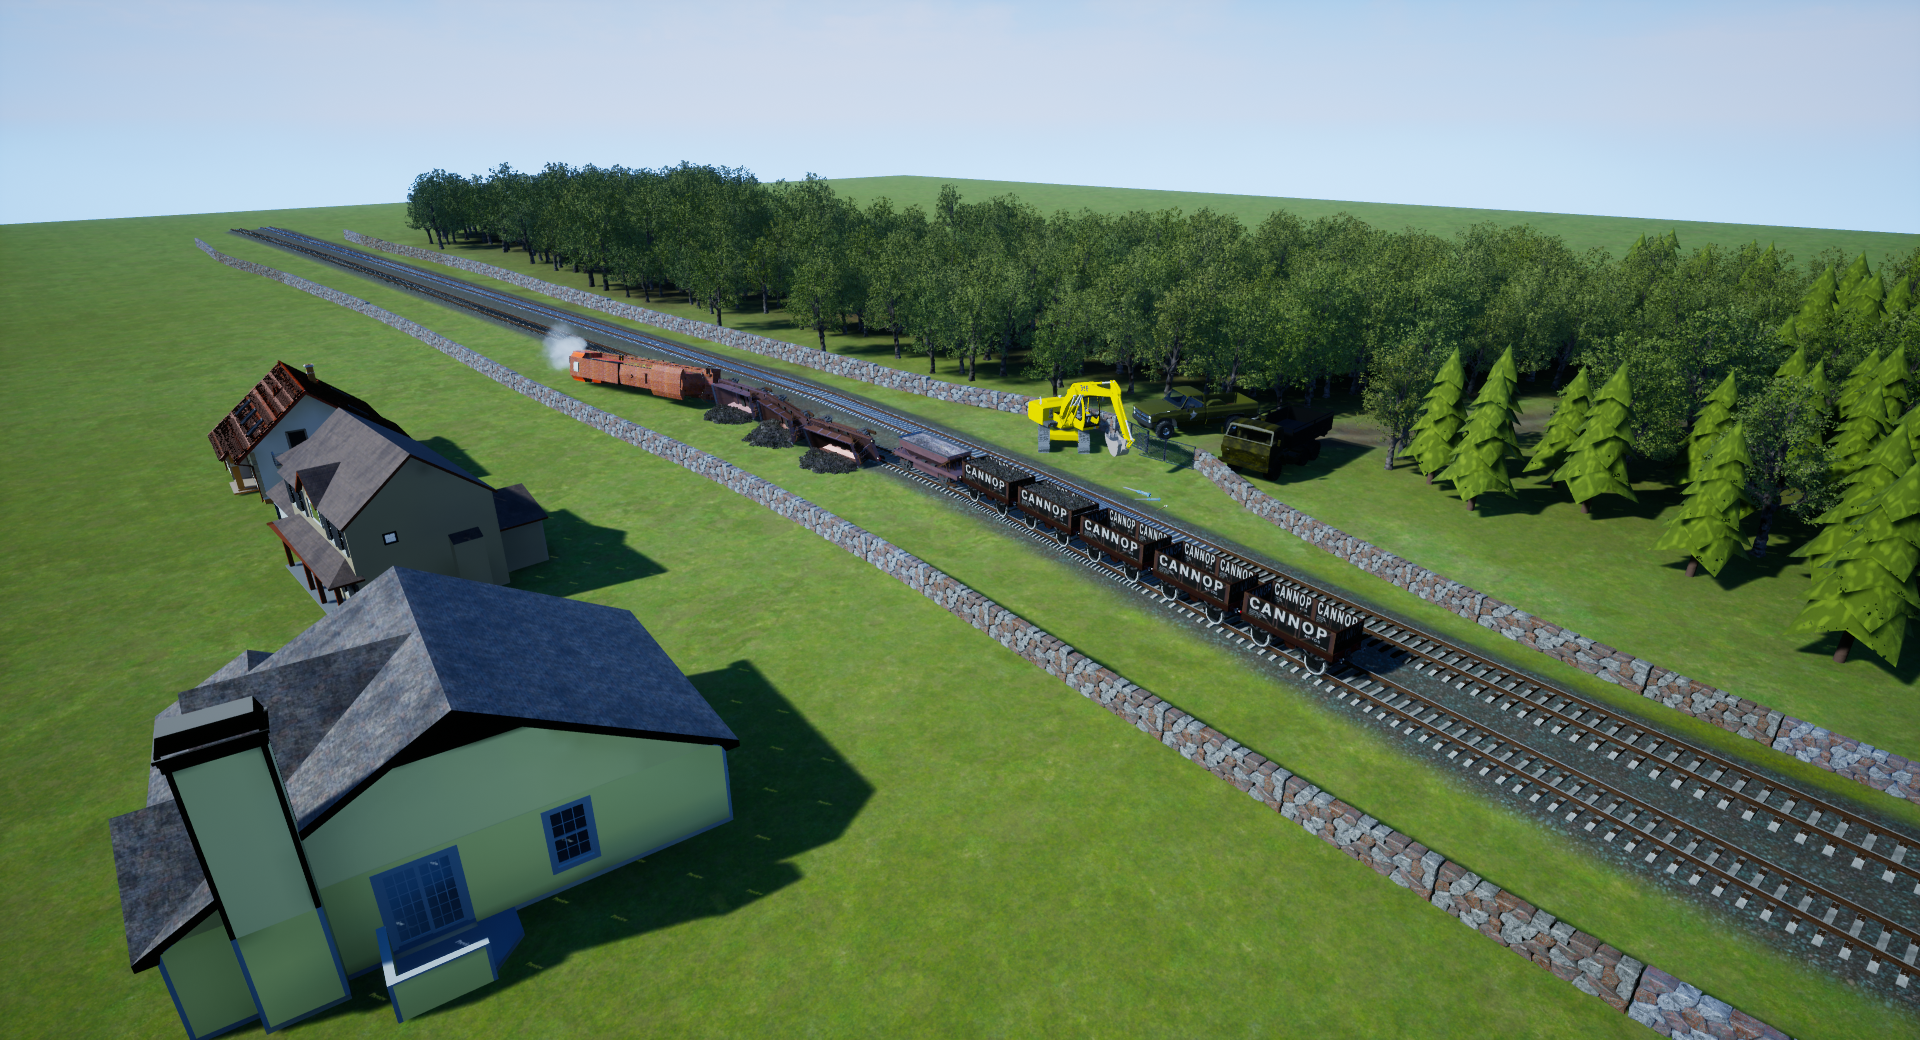
\includegraphics[width = 4.5cm]{Chapters/SimulationEnv/Figs/VirtualEnvV4/IsometricView2.png}} &
\subfloat[caption]{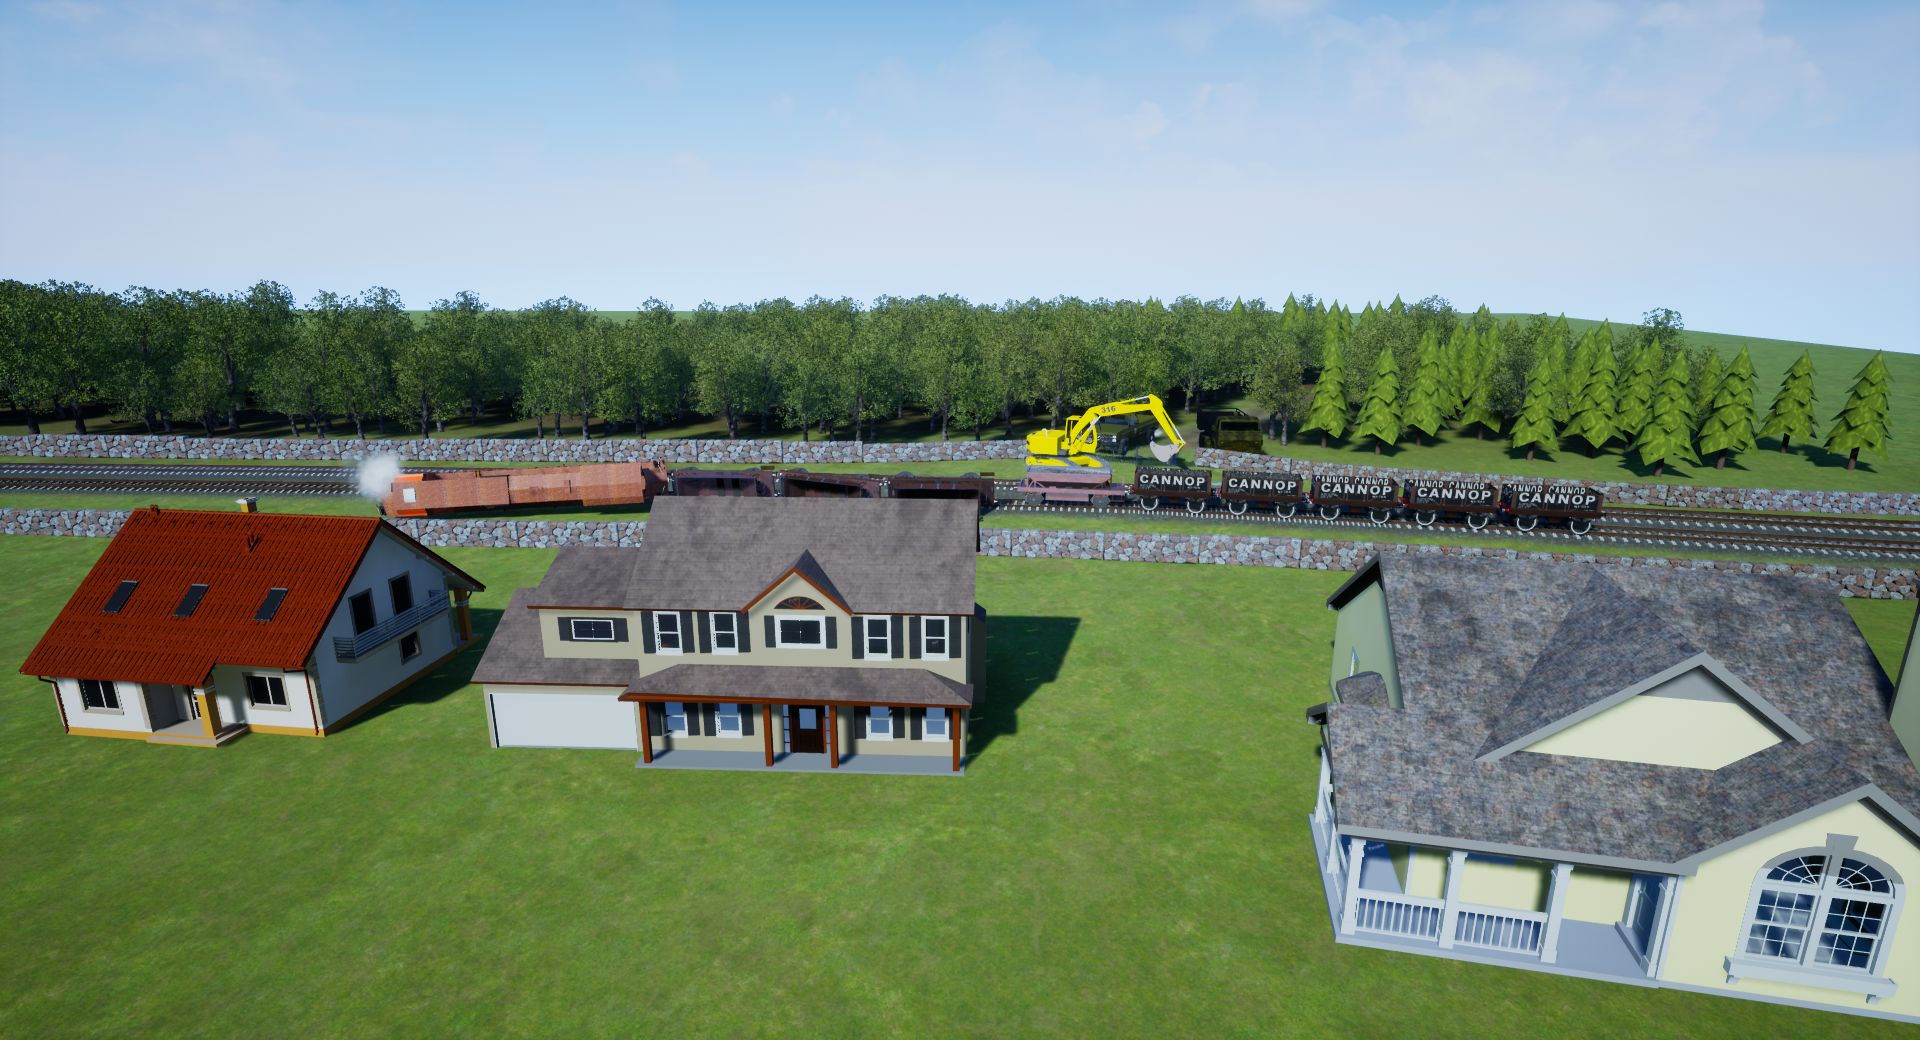
\includegraphics[width = 4.5cm]{Chapters/SimulationEnv/Figs/VirtualEnvV4/LowView2.png}}\\
%5thline of images
\subfloat[caption]{\includegraphics[width = 4.5cm]{Chapters/SimulationEnv/Figs/VirtualEnvV5/TopView.png}} &
\subfloat[caption]{\includegraphics[width = 4.5cm]{Chapters/SimulationEnv/Figs/VirtualEnvV5/IsometricView.png}} &
\subfloat[caption]{\includegraphics[width = 4.5cm]{Chapters/SimulationEnv/Figs/VirtualEnvV5/LowView.png}}
\end{tabular}
\caption{Evolution of Simulation Environment. Each row depicts images from a subsequent iteration.}
\end{figure}
\pagebreak



\note{Might not be necessary to talk about all of these things}

\begin{figure}
\label{fig:virutalEnvDevelopment}
\centering
\begin{tabular}{cc}
\subfloat{\includegraphics[width = 7cm]{Chapters/SimulationEnv/Figs/VirtualEnvFinal/IsometricView1.png}} &
\subfloat{\includegraphics[width = 7cm]{Chapters/SimulationEnv/Figs/VirtualEnvFinal/LowView.png}} \\

\subfloat{\includegraphics[width = 7cm]{Chapters/SimulationEnv/Figs/VirtualEnvFinal/TopView2.png}}&
\subfloat{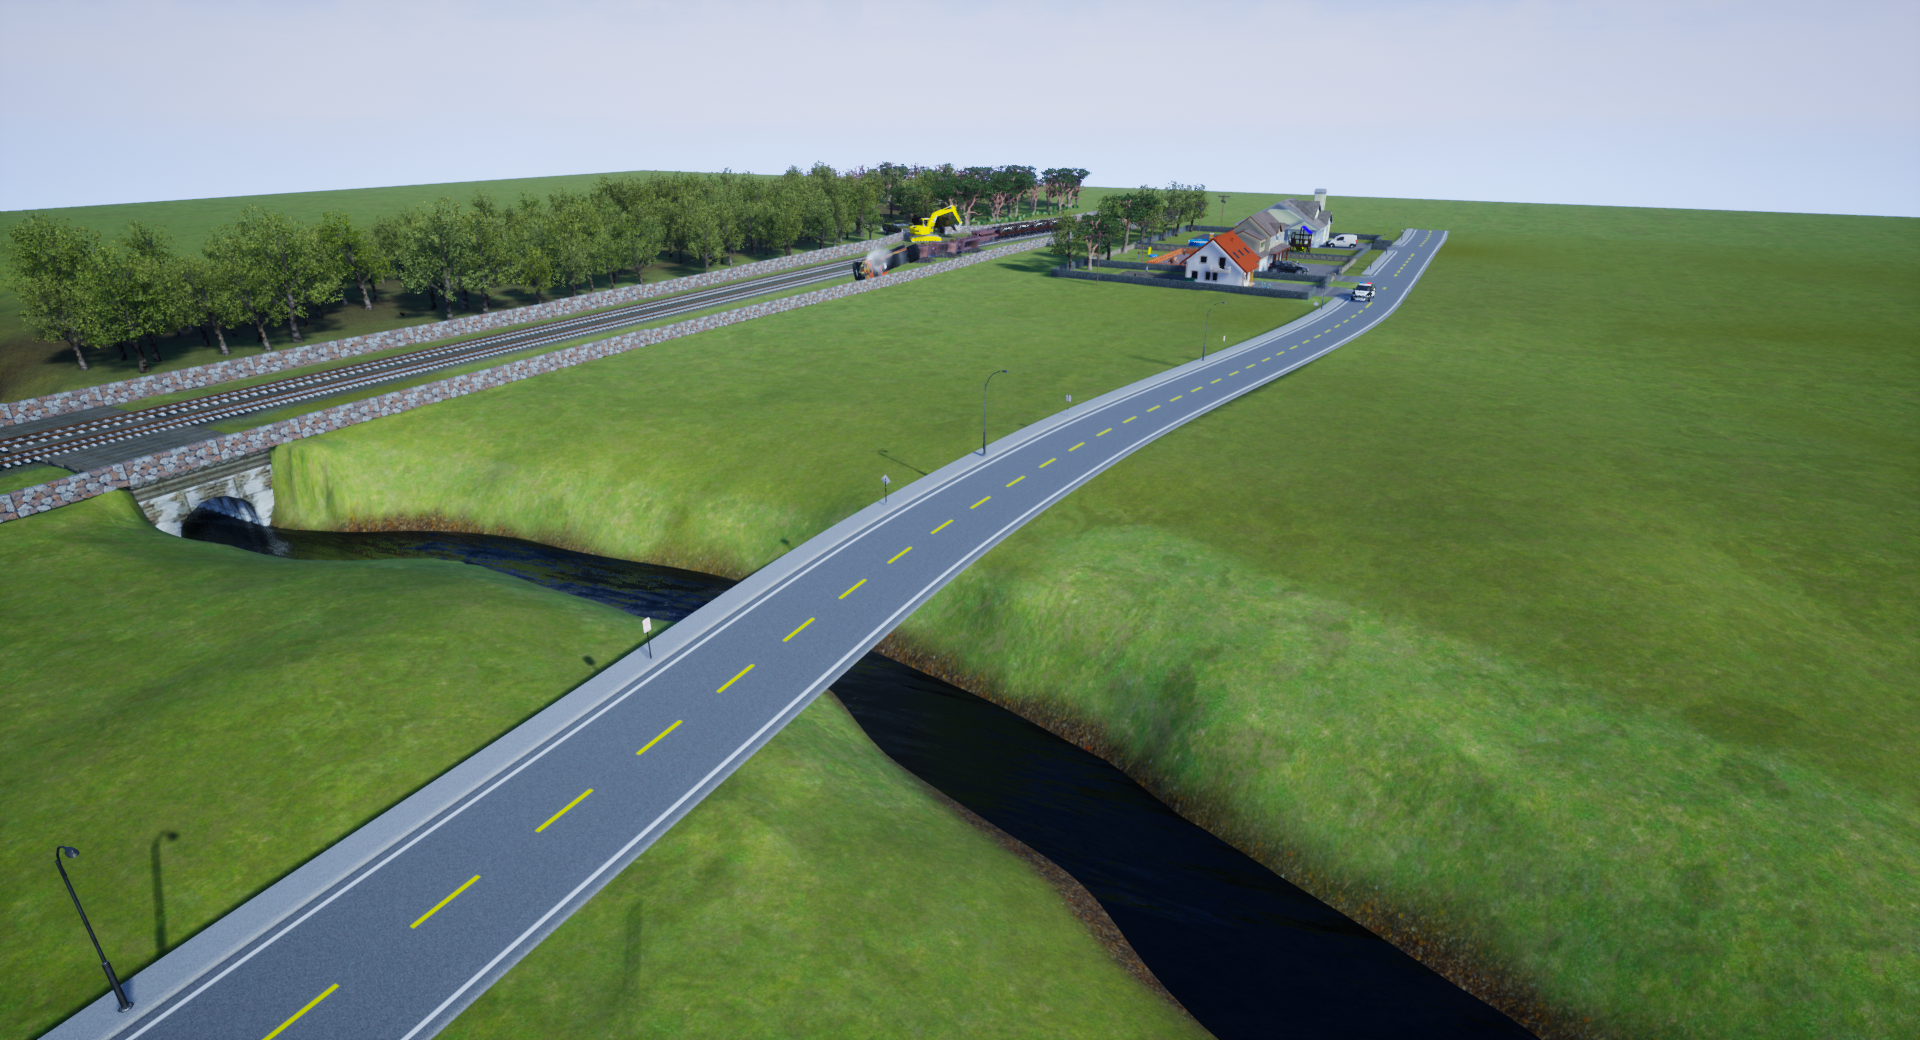
\includegraphics[width = 7cm]{Chapters/SimulationEnv/Figs/VirtualEnvFinal/BridgeView1.png}} \\

\subfloat{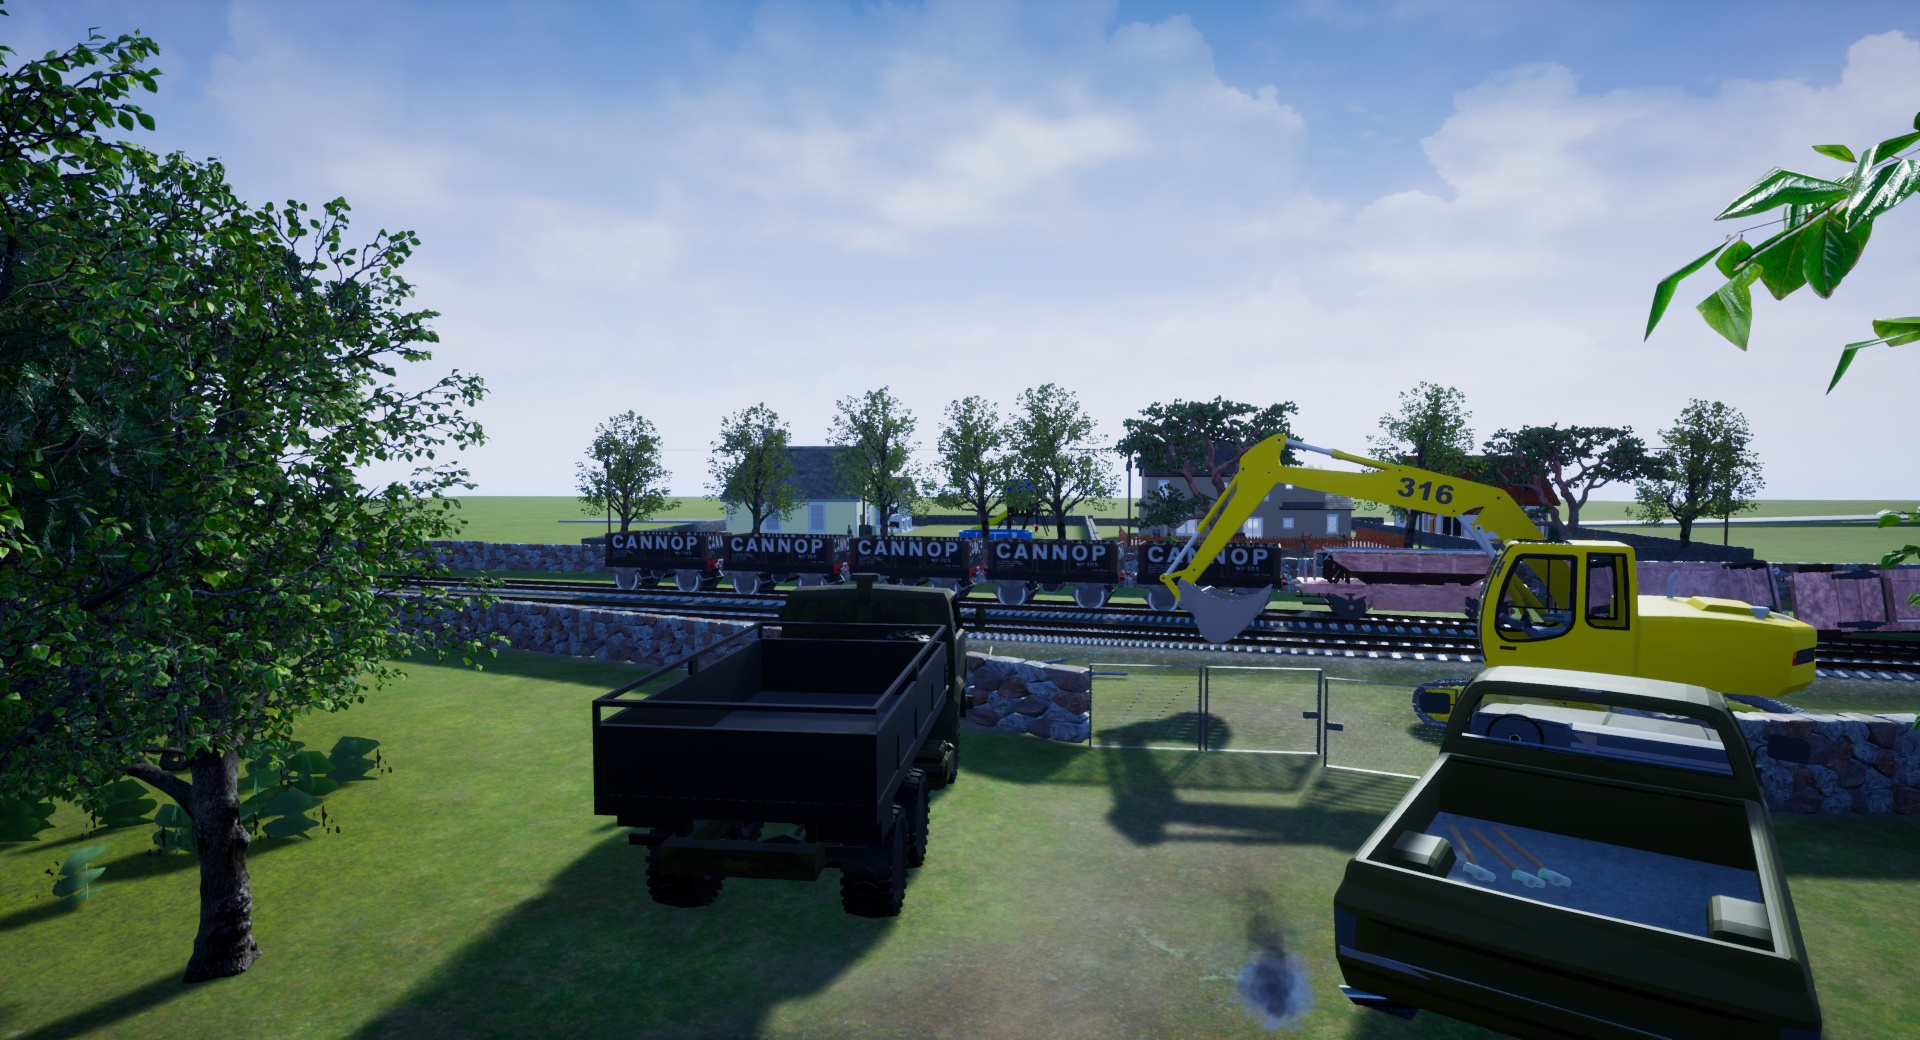
\includegraphics[width = 7cm]{Chapters/SimulationEnv/Figs/VirtualEnvFinal/CloseUp1.png}}&
\subfloat{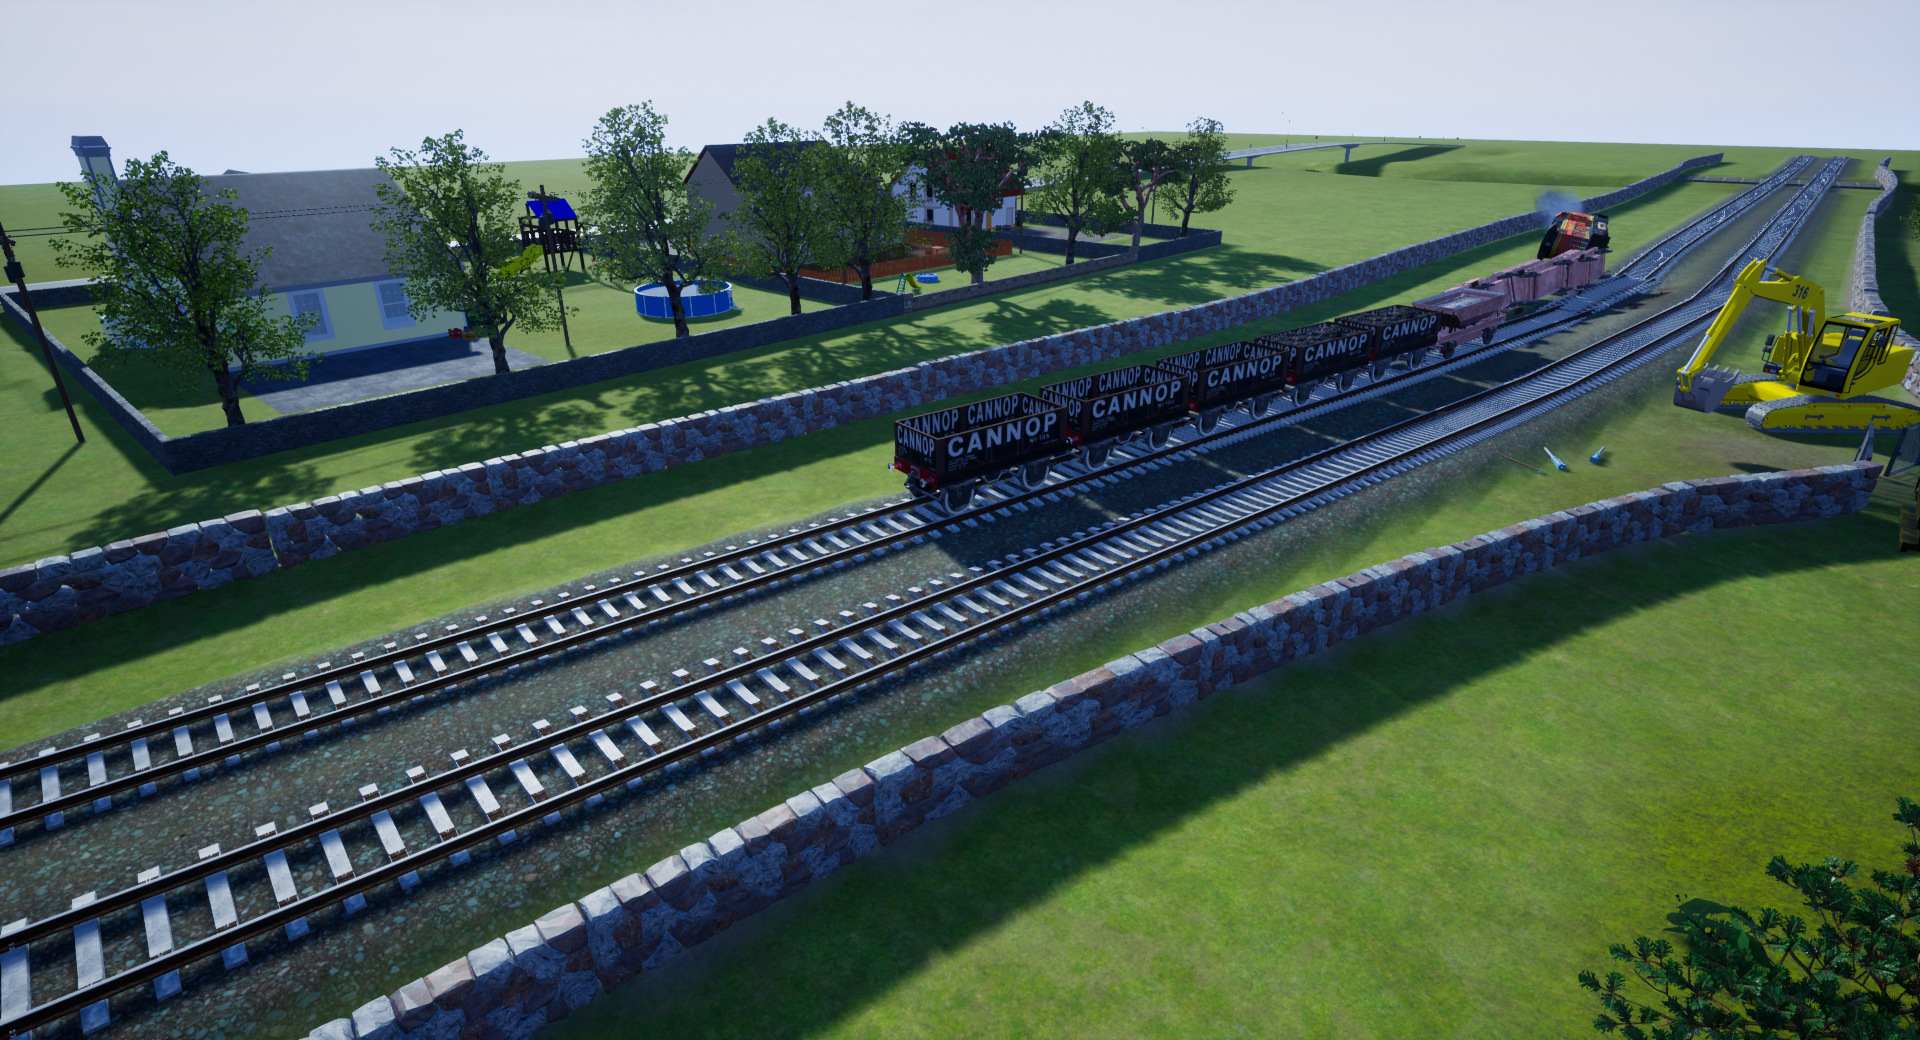
\includegraphics[width = 7cm]{Chapters/SimulationEnv/Figs/VirtualEnvFinal/CloseUp2.png}} \\
\end{tabular}
\caption{Final Version of Simulation Environment}
\end{figure}


\pagebreak
\begin{landscape}
\begin{figure}
\label{fig:virutalEnvDevelopment}
\centering
\begin{tabular}{cc}
\subfloat{\includegraphics[width = 9cm]{Chapters/SimulationEnv/Figs/VirtualEnvFinal/IsometricView1.png}} &
\subfloat{\includegraphics[width = 9cm]{Chapters/SimulationEnv/Figs/VirtualEnvFinal/LowView.png}} \\

\subfloat{\includegraphics[width = 9cm]{Chapters/SimulationEnv/Figs/VirtualEnvFinal/TopView2.png}} &
\subfloat{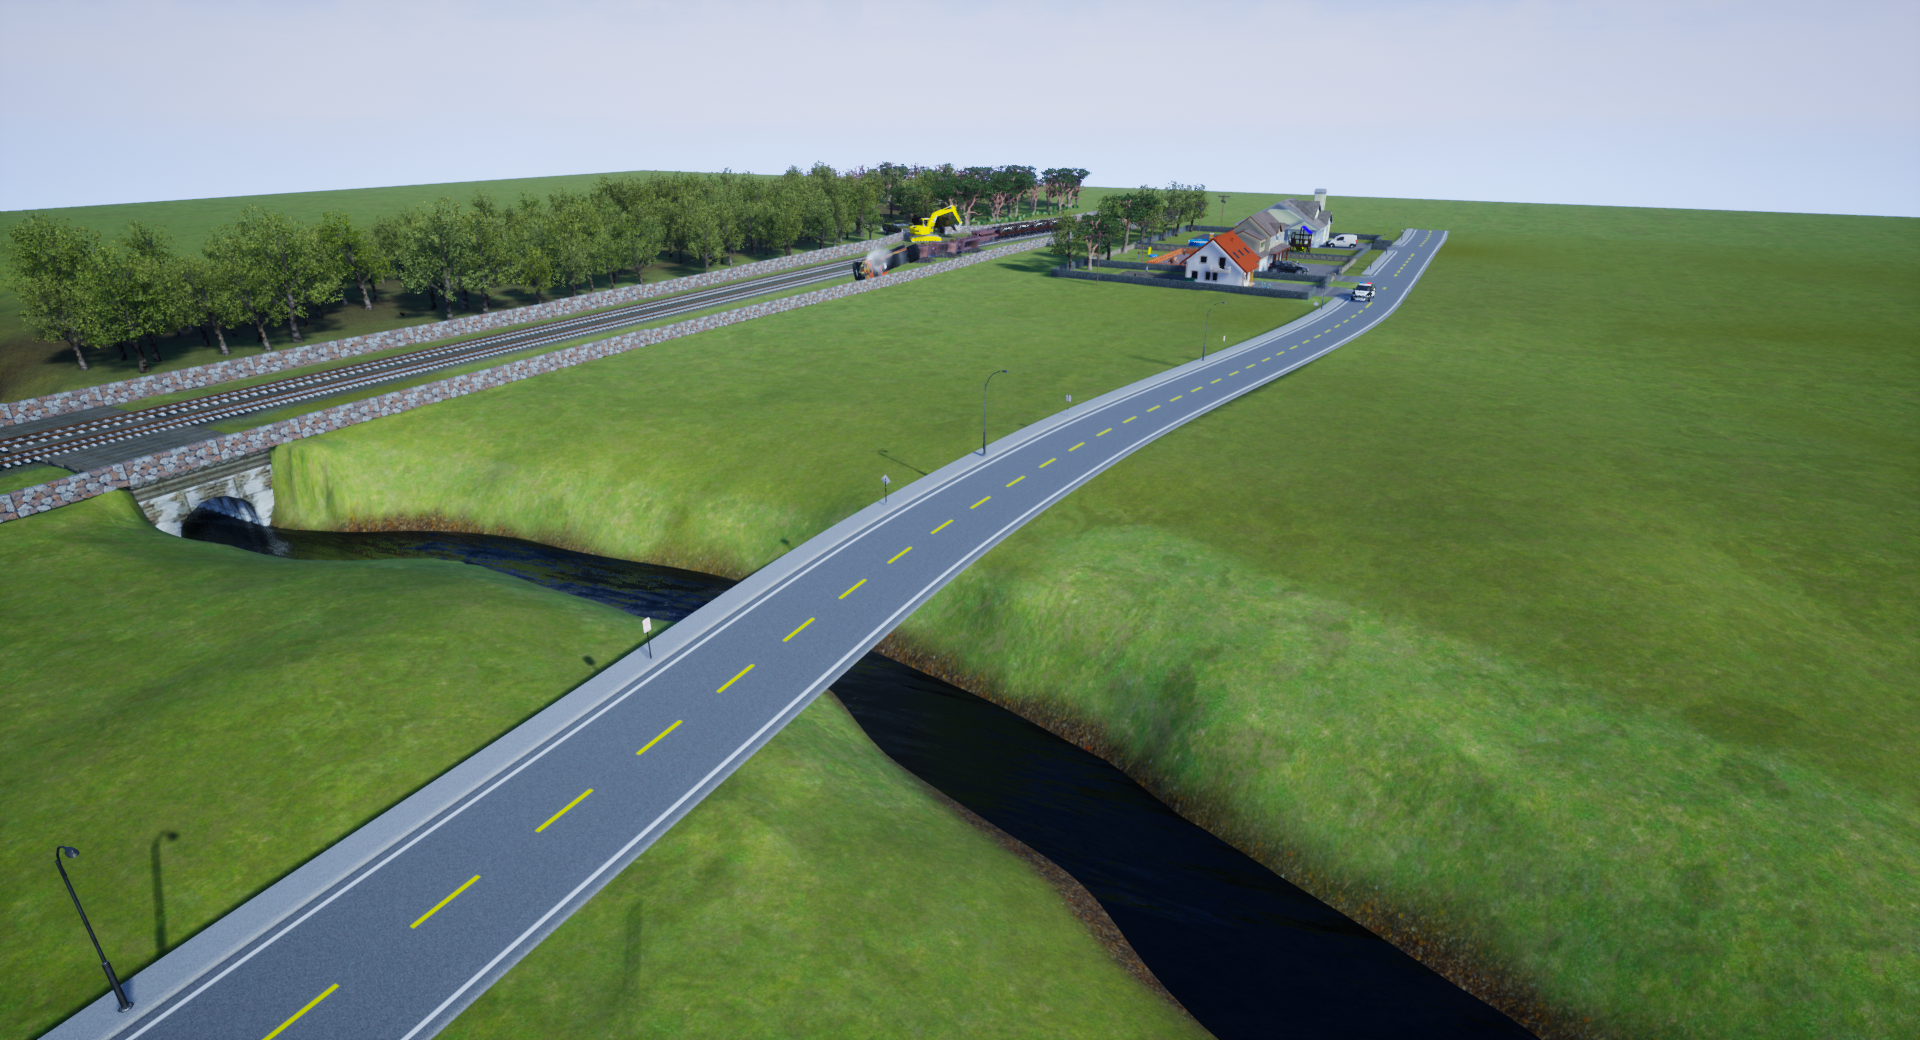
\includegraphics[width = 9cm]{Chapters/SimulationEnv/Figs/VirtualEnvFinal/BridgeView1.png}} \\

\subfloat{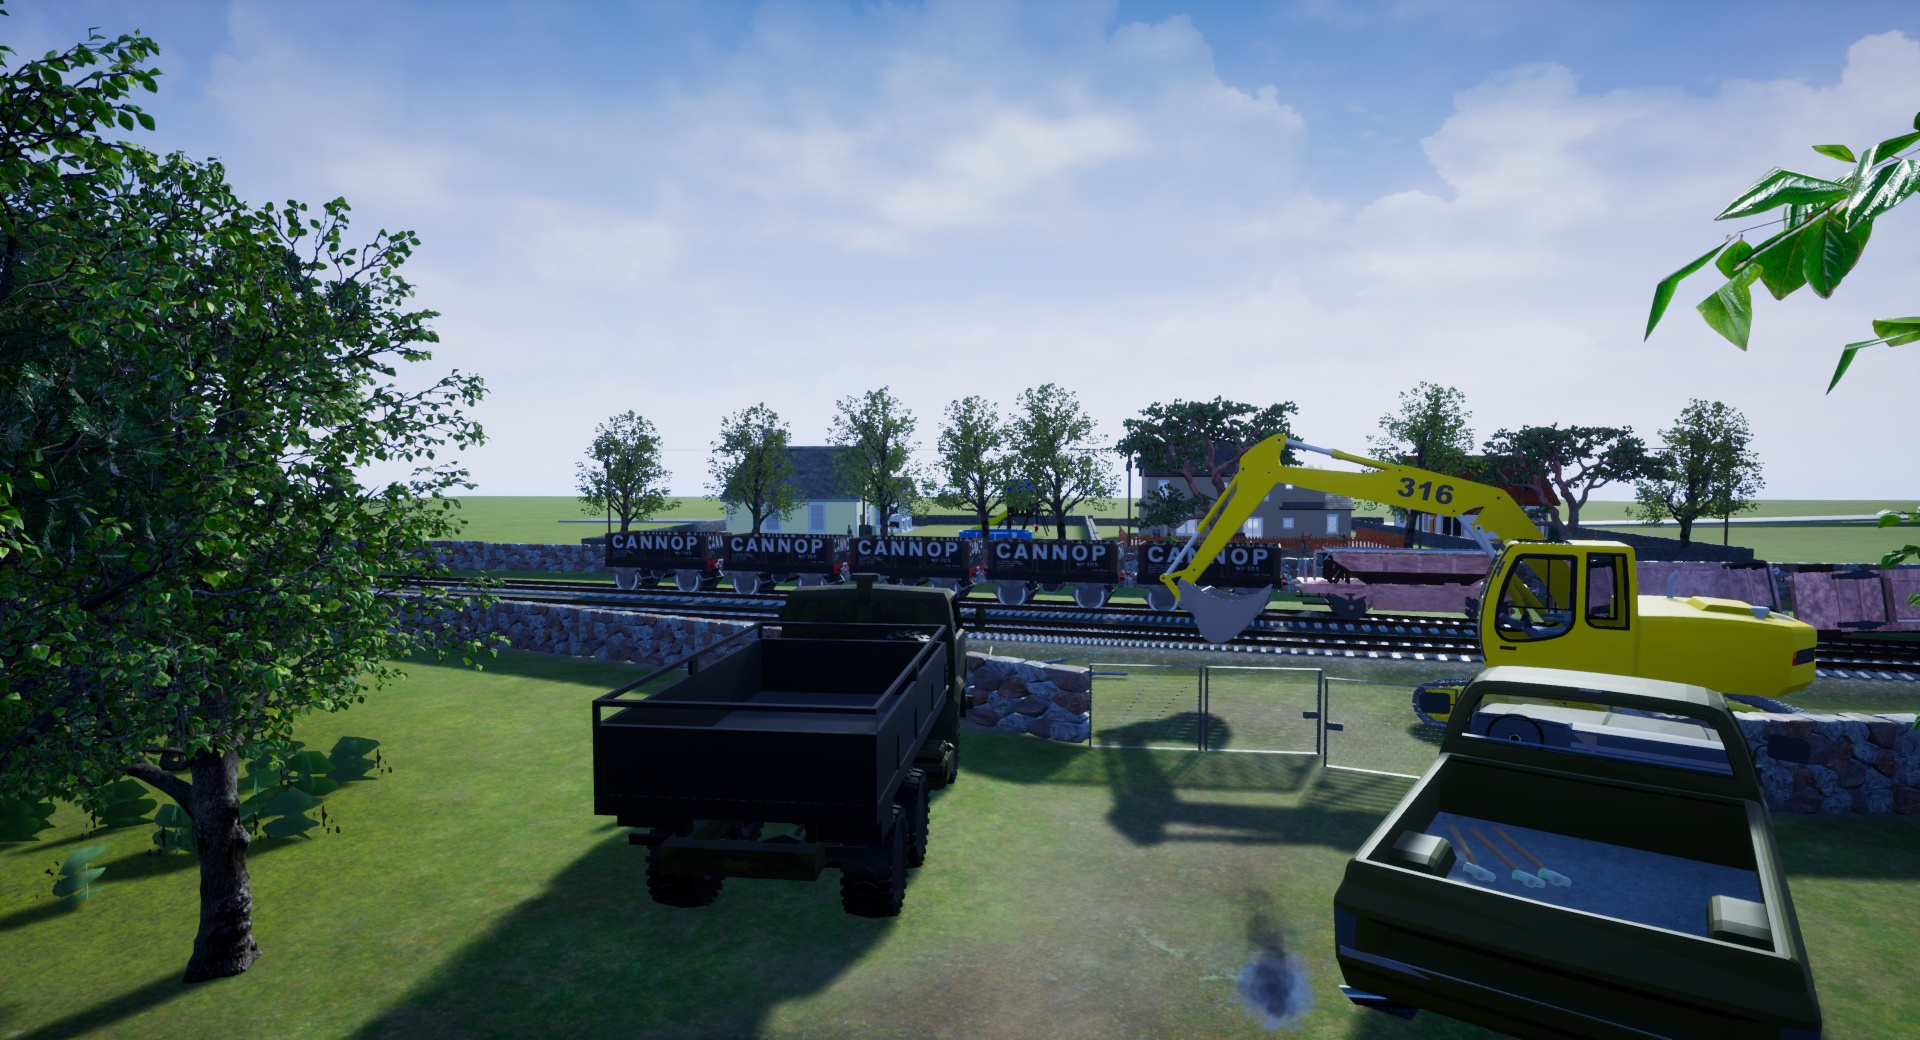
\includegraphics[width = 9cm]{Chapters/SimulationEnv/Figs/VirtualEnvFinal/CloseUp1.png}} &
\subfloat{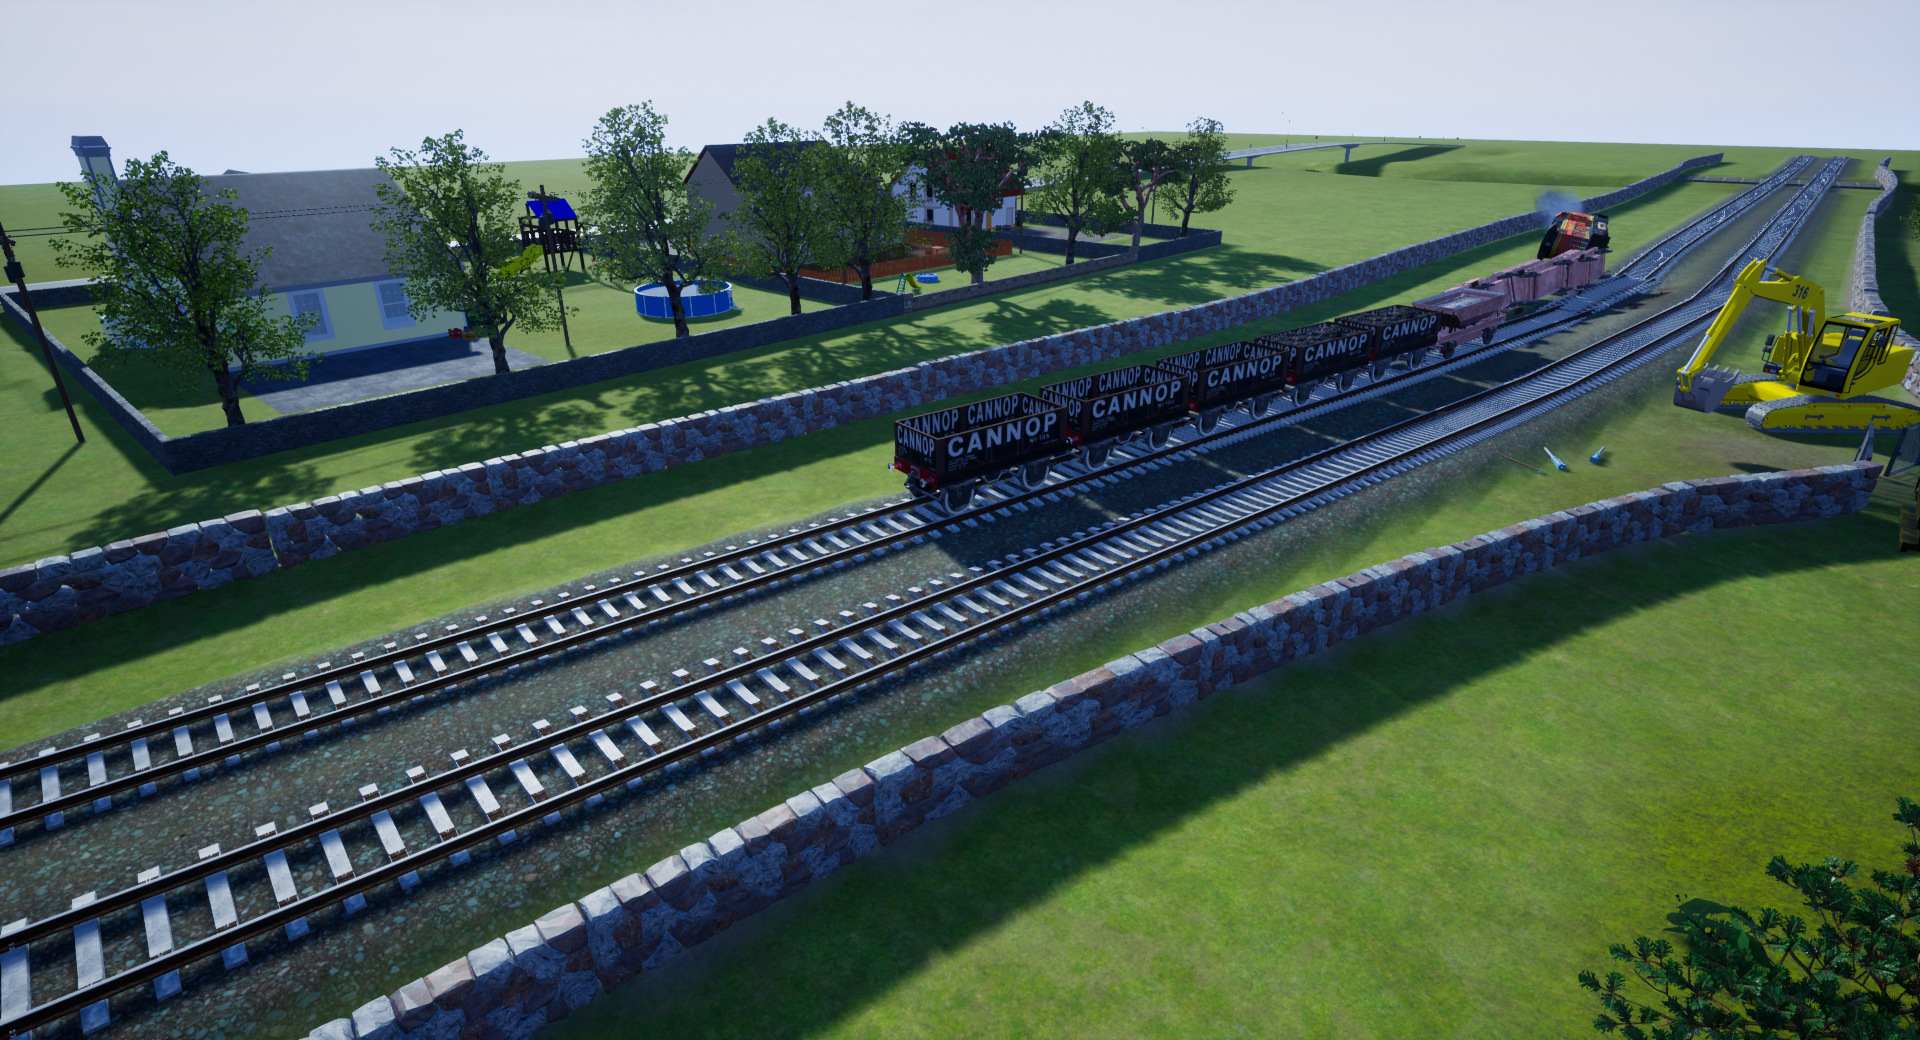
\includegraphics[width = 9cm]{Chapters/SimulationEnv/Figs/VirtualEnvFinal/CloseUp2.png}}
\end{tabular}
\caption{Images From Final Version of Simulation Environment}

\end{figure}
\end{landscape}
\pagebreak

\subsubsection{Blueprint Visual Scripting System}
UE4 uses a visual scripting system to provide a lot of functionality, known as Blueprints. Blueprints provide a node-based interface to create gameplay elements. In order to develop different aspects of a game, the system provides a visual approach to scripting, and many of the tools available in standard written scripting languages are available, such as typed variables, arrays, structs, loops, etc. Blueprints were used extensively in the subsequent sections, as well as C++ code, in order to develop the simulation.


\subsubsection{Materials}
\note{grass, rail tracks}

%\subfloat[caption]{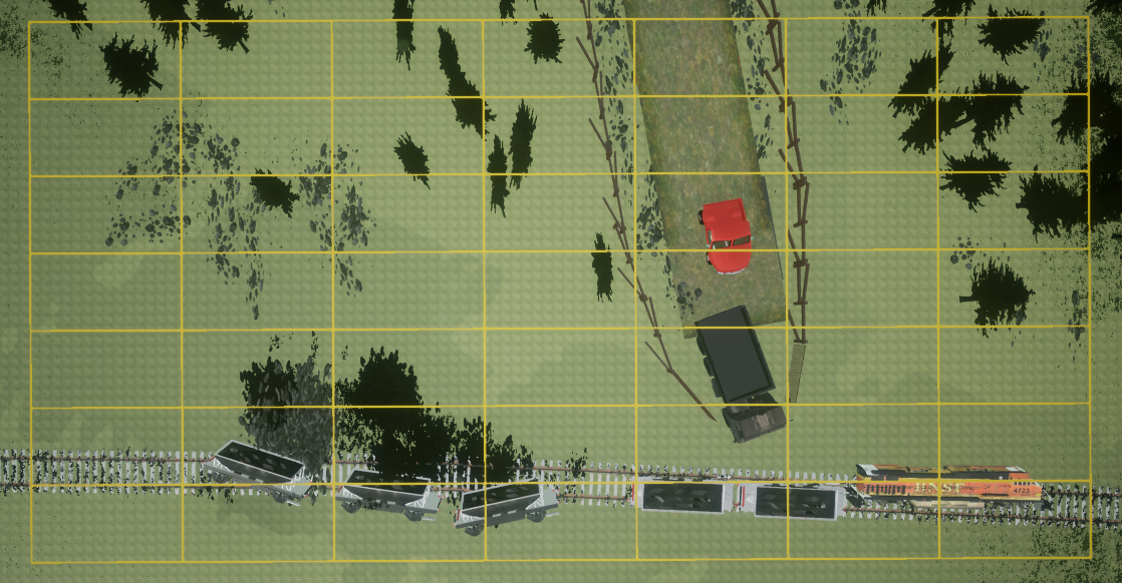
\includegraphics[width = 4.5cm]{Chapters/SimulationEnv/Figs/RailScenarioFirstIteration.png}} &
%\subfloat[caption]{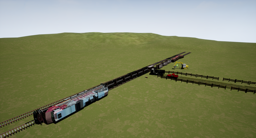
\includegraphics[width = 4.5cm]{Chapters/SimulationEnv/Figs/VirtualEnvV1/resized_HighresScreenshot00001.png}} \\

\begin{wrapfigure}{r}{0.4\textwidth}
    \centering
    \includegraphics[width=0.4\textwidth]{Chapters/SimulationEnv/Figs/BlendedMaterialsVSNotBlendedMaterials/PoorTextures.png}
    \label{fig:PoorTextures}
    \includegraphics[width=0.4\textwidth]{Chapters/SimulationEnv/Figs/BlendedMaterialsVSNotBlendedMaterials/HighQualityMaterial.png}
    \label{fig:GoodTextures}
    \caption{Contrast between initial and final materials used in simulation environment.}
\end{wrapfigure}

%https://docs.unrealengine.com/en-US/Engine/Rendering/Materials/IntroductionToMaterials/index.html
Materials are made up of a number of components in UE4, which specify aspects such as colour, opacity, roughness, specularity and emissive colours. In order to produce realistic materials, it is necessary to blend and layer different textures as well as identifying the correct parameters for surface normals and specularity, among the other features. UE4 has highly sophisticated tools for modifying materials to achieve a high-fidelity output. Details of creating materials can be found in the 
\href{https://docs.unrealengine.com/en-US/Engine/Rendering/Materials/IntroductionToMaterials/index.html}{UE4 Documentation}\footnote{\href {https://docs.unrealengine.com/en-US/Engine/Rendering/Materials/IntroductionToMaterials/index.html}{https://docs.unrealengine.com/en-US/Engine/Rendering/Materials/IntroductionToMaterials/index.html}}. The landscape in the first iteration of the virtual environment consisted of a single uniform texture, with none of the parameters mentioned above properly specified. The result of this is shown in figure \ref{fig:PoorTextures}. Subsequent versions used multiple layers and blending in order to create a higher-fidelity material, with relevant parameters tuned. This is shown in figures \ref{fig:LayerBlendNode} and \ref{fig:LandscapeMaterialBlueprint}, where a Landscape Layer Blend node is used to combine individual textures to create the landscape material.

\begin{figure}
\centering
\begin{tabular}{cc}
\subfloat[Layers blended into Landscape Layer Blend Node]{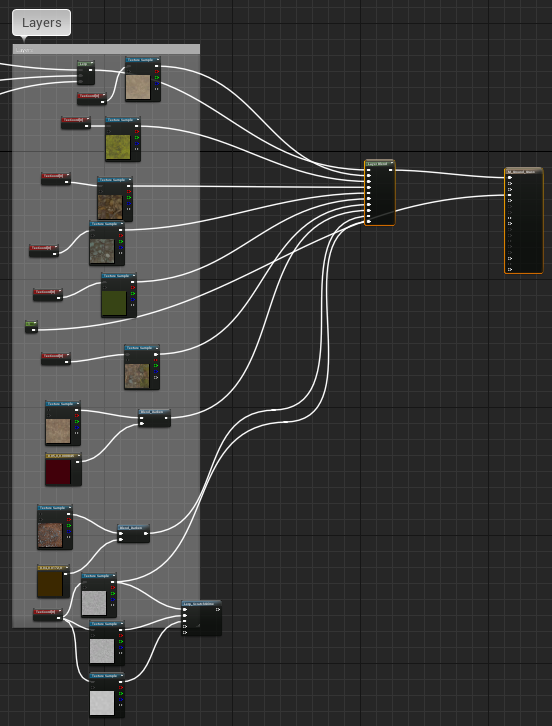
\includegraphics[width=4cm]{Chapters/SimulationEnv/Figs/BlendedMaterialsVSNotBlendedMaterials/LayerBlend.PNG}}\label{fig:LayerBlendNode} &


\subfloat[Blueprint used to create landscape material]{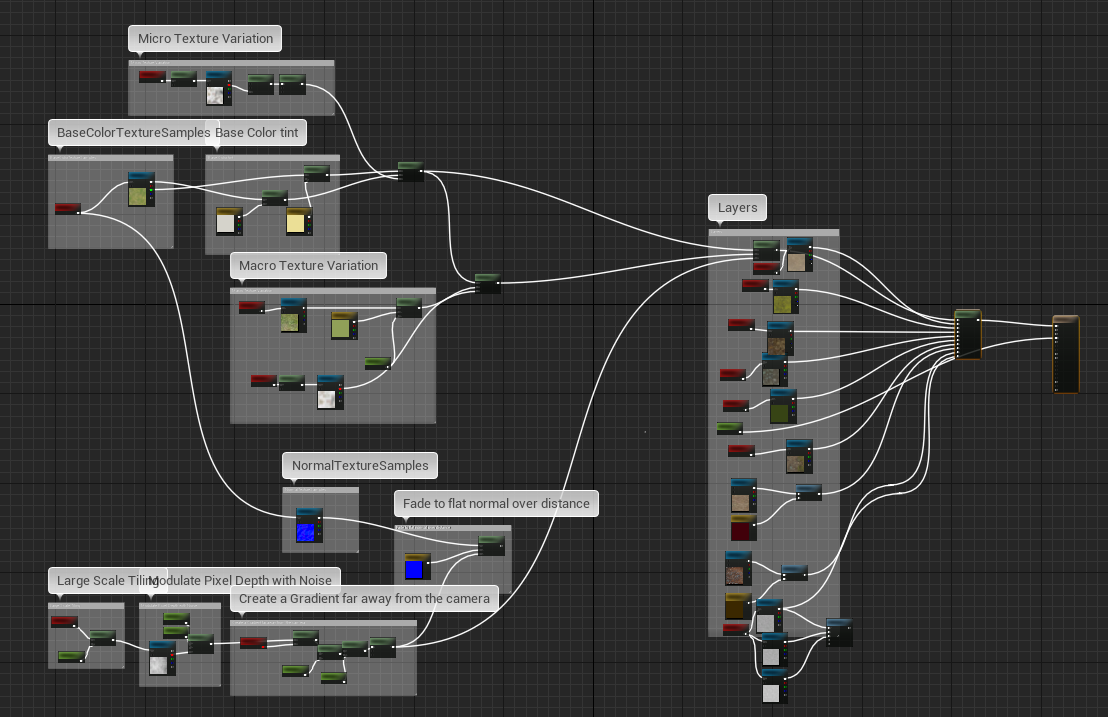
\includegraphics[width=4cm]{Chapters/SimulationEnv/Figs/BlendedMaterialsVSNotBlendedMaterials/LandscapeMaterial.PNG}}\label{fig:LandscapeMaterialBlueprint}
\end{tabular}
\caption{test}
\end{figure}


\subsubsection{Splines}

\begin{wrapfigure}{r}{0.4\textwidth}
    \centering
    \includegraphics[width=0.4\textwidth]{Chapters/SimulationEnv/Figs/SplineVSNoSplineExamples/PerfectlyStraightRail.png}
    \label{fig:StraightRail}
    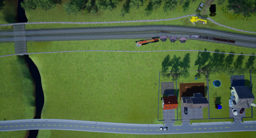
\includegraphics[width=0.4\textwidth]{Chapters/SimulationEnv/Figs/SplineVSNoSplineExamples/resized_SplineExample1.png}
    \label{fig:SplinedRail}
    \caption{Contrast between initial and final materials used in simulation environment.}
    
\end{wrapfigure}

Uniformity tends to be rare in the real world; perfectly straight lines don't often occur naturally. For this reason UE4 offers tools to create splines, along which the terrain can be deformed. Splines are typically used to model roads and paths, but the Landscape Spline system is very flexible and can be used to model many different phenomena. In the initial stages of the simulation environment, only a perfectly straight section of rail could sourced for use in the environment, as shown in figure \ref{fig:StraightRail}. The spline tool allowed for much more realistic construction of the section of rail and accompanying wall, as shown in figure \ref{fig:SplinedRail}. It was also used to create the road and the bridge section. \note{maybe provide link to docs}


\subsubsection{Foliage}
Similar to the argument made in relation to splines, it is rare to have uniformly configured foliage in the real world. In order to address this, there exist foliage generation and editing tools in UE4 editor. Version 4.18 of the editor onwards contains the Procedural Foliage Tool \note{maybe add a link}, which is the most convenient way to add swathes of foliage to a scene. Since we were using other content dependent on UE 4.16, we opted to use the foliage painter tool, which allows the user to effectively paint foliage directly onto a landscape. It allows the user to specify a number of parameters to achieve the required density, scaling and other relevant features. The results of applying foliage to the scene are visible in figures \ref{}, \ref{} and \ref{} respectively.
\note{Non-uniform trees, grass, etc.}

\begin{figure}
\centering
\begin{tabular}{ccc} 
\subfloat[Layers blended into Landscape Layer Blend Node]{\includegraphics[width=4cm]{Chapters/SimulationEnv/Figs/Foliage/Foliage2.png}}\label{fig:LayerBlendNode} &

\subfloat[Blueprint used to create landscape material]{\includegraphics[width=4cm]{Chapters/SimulationEnv/Figs/Foliage/Foliage5.png}}\label{fig:LandscapeMaterialBlueprint} &
\subfloat[Blueprint used to create landscape material]{\includegraphics[width=4cm]{Chapters/SimulationEnv/Figs/Foliage/Foliage6.png}}\label{fig:LandscapeMaterialBlueprint}
\end{tabular}
\caption{test}
\end{figure}

\subsubsection{Landscape Editing}
\note{Discuss here how dirt track was created using}
Creating a realistic landscape in UE4 serves a number of purposes. In order to allow the potential simulation of the operation of ground vehicles, it is necessary to model the terrain realistically so that difficulties that may be experienced in the real world, such as steep climbs or highly uneven surfaces, may be taken into account. UE4 provides a suite of landscaping tools that allows the user to create a highly variable landscape. The tools facilitate raising and flattening, smoothing, random noise and simulated erosion, as well as allowing for other more detailed modifications. These were used to create the railway embankment, the rutted path leading onto the rail tracks and the riverbank and riverbed, shown in figures \ref{}, \ref{} and \ref{} respectively.

\begin{figure}
\centering
\begin{tabular}{ccc}
\subfloat[Rutted Track]{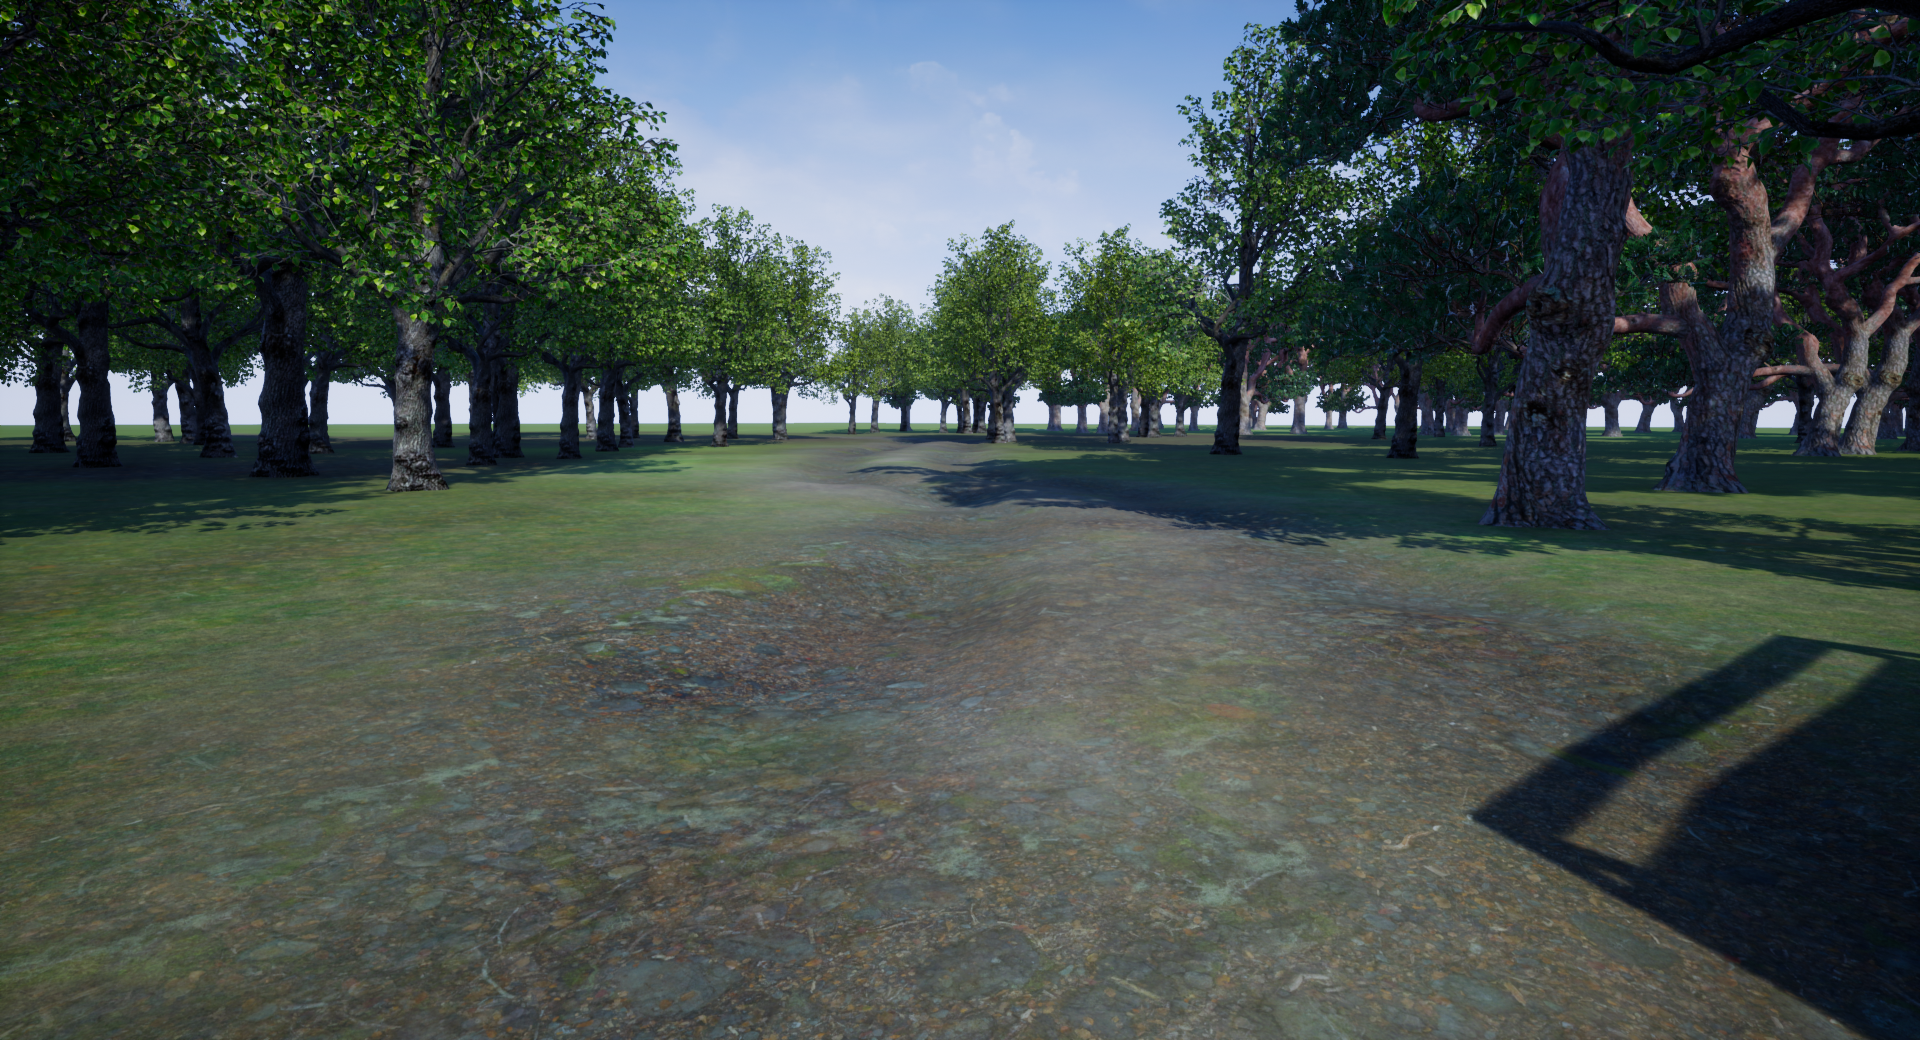
\includegraphics[width=4.5cm]{Chapters/SimulationEnv/Figs/LandscapedVSNotLandscaped/RuttedTrack.png}}\label{fig:RuttedTrack} &


\subfloat[Rail embankment]{\includegraphics[width=4.5cm]{Chapters/SimulationEnv/Figs/LandscapedVSNotLandscaped/RailwayEmbankment.png}}\label{fig:LandscapeMaterialBlueprint} &

\subfloat[Riverbank]{\includegraphics[width=4.5cm]{Chapters/SimulationEnv/Figs/LandscapedVSNotLandscaped/Bridge.png}}\label{fig:LandscapeMaterialBlueprint}

\end{tabular}
\caption{test}
\end{figure}

\subsubsection{Asset Sourcing}
An asset can be described as a piece of content for an Unreal Engine project, which has been serialized to a file. Assets can be re-used and modified in the UE4 editor, but are usually created using external software. UE4 uses assets that come in the Filmbox (.fbx) format, which is a proprietary file format owned by Autodesk\note{Do I need to reference this?}. Conversion tools do exist from other common asset file formats to fbx, but results can vary. Due to limited funding, time and experience, we decided to avoid creating assets from scratch but rather used assets that were free to use. Searching for free assets is a labor-intensive process, as it consisted of a number of steps:
\begin{enumerate}
    \item First, identify possible candidates for a particular type of asset (e.g. a train) based on a search of asset stores that offer free assets. We mainly used \href{https://www.cgtrader.com/}{CGTrader}\footnote{\href {https://www.cgtrader.com/}{https://www.cgtrader.com/}} ,
    
    \href{https://www.turbosquid.com/}{TurboSquid}\footnote{\href {https://www.turbosquid.com/}{https://www.turbosquid.com/}}
    , 
    \href{https://3dwarehouse.sketchup.com/?hl=en}{3D Warehouse}\footnote{\href {https://3dwarehouse.sketchup.com/?hl=en}{https://3dwarehouse.sketchup.com/?hl=en}} 
    and
    \href{https://www.shapenet.org/}{ShapeNet}\footnote{\href {https://www.shapenet.org/}{https://www.shapenet.org/}}.
    
    \item Once a potentially suitable asset had been identified based on it's description and preview, it was downloaded in the Filmbox (fbx) format if possible. Otherwise, it was downloaded in whatever format was available. 
    \item The asset was opened in Autodesk \note{add reference} and visually inspected for suitability. If the textures and geometry were not of a sufficient standard the processes was restarted.
    \item If the asset was deemed suitable from the inspection in Autodesk, then it was exported in Filmbox format.
    \item The asset was then imported into the UE4 editor. Problems often arose in scaling, incorrect texture mapping and one-sided materials applied to the wrong side of assets. These problems could sometimes be addressed; if not we had to restart the process.
\end{enumerate}

\subsubsection{Shadows}
\note{This might not be worth talking about. almost Everything is provided by default}


%Talk about how well static world matches specification, how well rendered images perform for training some object detection etc.
%Also talk about how the environment was packaged and open-sourced with permissive licence for general use



% Not sure of exact ordering here
% 1st Iteration J:\Work\David\ROCSAFEMidTermDemo\Code\UnrealEngine\AirSim\Unreal\Environments\Blocks
% 2nd Iteration J:\Work\David\UnrealEngineRocsafe\OS_01RadIntegr
% 3rd Iteration D:\ROCSAFEScenarios\OS01TestTemp
% 4th Iteration D:\ROCSAFEScenarios\OS_01Radiation - D:\ROCSAFEScenarios\OS_01Radiation\Saved\Screenshots\Windows screenshot 11
% 5th \\ROCSAFE2\ROCSAFEGroupShared\ROCSAFEUnrealEngineOperatingScenarios\NotIntegratedAirSim

% V1: Brussels Demo
% V2: Rail with spline, train, digger. No dirt track, no houses, no road, no wall, poor textures, poor foliage
% V3: Add wall, better foliage
% V4:and houses
% V5: Proper foliage (stones) & blended textures
% V6: Final version in shared folder


\section{Virtual Aerial Vehicle Integration}

\section{Radiation Simulation}

\section{Qualitative Coverage Problem Test Results}

\section{Quantitative Target Detection Test Results}

\section{Future Work}
%!TEX root = ../thesis.tex
%*******************************************************************************
%****************************** Third Chapter **********************************
%*******************************************************************************
\chapter{Multi-Agent Coverage Problem}



%Contains the restructured agent design etc.

\chapter{Multi-Agent Stochastic Target Localization}\label{chap:targetLocalisation}
\workinprogress
This chapter outlines the approach taken to solve the research question stated in the introduction chapter. The context for this problem is derived from the ROCSAFE project \cite{rocsafeNUIG}. \note{Not sure how best to present the problem and how to provide the necessary content to naturally leads to the approaches discussed here. Fill this out further once research questions have been finalized/refined}


\section{Problem Description}\label{sec:TLocalisationProbDescription}
As mentioned in Chapter \ref{chapter:introduction}, a major problem in hazardous scene management includes localizing sources of hazardous materials and localizing potential sources of evidence. The reasons these are difficult problems, in the context of the ROCSAFE project, are:
\begin{itemize}
    \item Hazardous materials belong to different classes of threat (chemical, biological, radiation, nuclear). If the nature of the threat is uncertain, the wrong preventative measures may be taken and personnel may be put at risk. 
    \item Evidence localisation usually requires moving a sensor to within close proximity of the evidence. If a human is responsible for this, there is a chance that they will accidentally disturb with the evidence, possibly yielding it unusable.
    \item Since these scenarios are highly dangerous, the area to search may be large to avoid potentially missing important sources of evidences. This means that the process of localisation may be painstaking and time-consuming for humans.
\end{itemize}
In the ROCSAFE project, the use of RAVs is proposed to aid the execution of these tasks \cite{Bagherzadeh2017ROCSAFE:Incidents}. This chapter proposes a system to aid their navigation planning.

  
%This section proposes a system that can aid the execution of these tasks using a system of automated \textbf{U}nmanned \textbf{A}erial \textbf{V}ehicles (RAVs). \par



Spatiotemporal localisation problems have a reasonable body of literature behind them, and can be described using abstract language which allows them to be approached using a common framework, with only minor implementation details necessary to specify which instance of the problem is being addressed. The framework we have developed uses a lot of the theory outlined in Chapter \ref{chapter:Background} and builds on the literature that was reviewed there. The problem that this Chapter attempts to solve can be generally described as follows: \par

\textit{Given a region of space to explore and a set of heterogeneous autonomous aerial vehicles with sensing capabilities, devise a search strategy with a search cutoff criterion which will accurately return either the locations of the targets if one or more is present, or return that no targets are present, in the shortest possible time.} \par

We designed the system to be general, but we list some concrete versions of this problem that we envisage this approach could effectively solve:
\begin{itemize}
    \item \textit{Given a system of heterogeneous autonomous aerial vehicles, some of which are equipped with radiation sensors and limited battery capacity, localize multiple sources of radioactive material in a scene.}
    \item \textit{Given a system of heterogeneous autonomous aerial vehicles, some of which are equipped with high-quality cameras and limited battery capacity, localize multiple objects of a given description in a scene.}
\end{itemize}
Note that we do not give the details of how to solve these specific instances of the problem.
%not sure whether I should mentioned about battery etc. here or to let the discussion lead to this naturally.
\par
%In order to solve this problem, we took an approach suggested by previous works in the literature \cite{PollockSearchInterfaces} <add more here>, which break down the localisation problem into phases, between which we consider interfaces that allow the composition of various methodologies to be applied. The literature review behind this is outlined in section <reference the section>.


%\note{Did not attempt to solve this full problem in one go, instead took a simplified version and then gradually added in constraints.}

\subsection{Initial Assumptions}
\note{may need to rename this. want to convey that initially, we made some simplifying assumptions that isolate key aspects of problem that need to be solved. Then these assumptions were modified to deal with the more complex problem involving battery etc.}

Rather than immediately attempting to tackle the full problem, we chose to initially make some simplifications in order to identify potential solution strategies that could be extended to more complex versions of the problem. At the outset, we made the following simplifying assumptions:
%As outlined in the literature review, this problem has been approached before by treating the problem as a 2 Time Slice Dynamic Bayesian Network (2TDBN). 
\begin{itemize}
    \item There are either zero or one targets to be localized.
    \item The UAVs have unlimited battery capacity.
    \item The region that the UAVs need to search can be well approximated by a polygon.
    \item The sensor specificity and sensitivity are known or can be estimated for a given resolution (e.g. 1m). These are assumed to be greater than 50\% for the given resolution.
    \item The UAVs operate over a discrete spatial grid spanning the region to search, assumed to be polygonal as above, the dimensions of which are pre-determined by the sensor resolution.
    \item The UAVs are assumed to have a GPS sensor that is accurate to beyond the sensor resolution (implying that the UAV moves to discrete grid locations without drift).
    \item The target is assumed to be small enough to occupy only one grid cell at a time. It is also assumed to not lie across grid cells.
\end{itemize}
While these assumptions are clearly unrealistic, they are convenient because they simplify the design of the system and subsequent analysis. In later sections in this chapter, these assumptions are relaxed and the necessary modifications for the solution strategy are discussed. Some ramifications of these assumptions are addressed later in the chapter, at section <x>. It is worth noting that similar simplifying assumptions were made in related works in the literature, 
(\cite{Chung2007ASearch} and \cite{Waharte2010SupportingUAVs}), % find additional citations in mendeley
which strongly influenced our initial approach.

\subsection{Experimental Testbed}
Given the assumptions outlined above, rather than beginning by working on designing candidate solutions, we instead decided to set up the software that would be necessary to quickly test and evaluate a solution. This is related to the specification of the agent's environment, which is described in subsection \ref{subsection:intial_agent_design}. This involved the following software components:
\begin{itemize}
    \item A 2-Dimensional grid coordinate system which can be easily configured to create a grid over a polygonal region. This is outlined in greater detail in section <provide a reference to the section>.
    \item An evidence source simulator which simulates the readings that a sensor would observe given the sensitivity and specificity of the sensor.
    \item A grid manager component, which manages the positions of RAVs and targets on the grid.
    \item A simulation manager component, which constructs the agents from their configuration files and is responsible for running the simulation using the other software components.
    \item Configuration files which allow the user to specify the configurations of the sensors, the agents, environment parameters and debugging/analysis files.
\end{itemize}
These components were designed in a modular fashion to distinguish the agent from its environment, shown in Figure \ref{fig:agent_env_interaction}. This seems like an obvious and intuitive practice, but can be easily overlooked while writing code. For example, the agent may have an internal representation of the grid environment in which it operates which should be completely independent of the actual grid environment which is run in the simulation. The user can fully specify all aspects of the agent and environment (relating to the above assumptions) through configuration files. \note{Maybe include an example figure showing a config file.}



%This file contains all the details of agent design using files in initialAgentDesign folder




\section{Agent Design}\label{section:intial_agent_design}
\note{addressed some of these simultaneously (i.e. once I had decided model-based agent, then had to answer question of what model will look like)}
\note{probably best to list these individually with some corresponding discussion}

When designing the agent, we adhered the approach outlined in Chapter 2 of "\textit{Artificial Intelligence: A Modern Approach}" \cite{AIAMA}. First, we describe four critical parts of the agent design, collectively referred to as the agent's \textit{task environment}: the Actuators, Sensors, Environment, and Performance Element. Further discussion on specific aspects of how the agent function was implemented is then given.
%where the larger multi-faceted problem is broken down into smaller individual sub-problems. 

\subsection{Agent Environment}
\note{Use of italics may not be necessary here}
\note{Should refer to previous works more here}
Here, we refer to conventional terms used to describe agent environments, described in \cite[p.~41]{AIAMA}. The agent's environment is \textit{partially observable}, since it is assumed that it cannot directly observe the location of the target, but must instead use partial information related to the location of the target from noisy sensors. The outcomes of the agent's actions are assumed to be \textit{deterministic}, meaning that if an agent chooses to move to a location, it is assumed to do so without any chance of it accidentally moving to an alternative location. The environment is \textit{sequential}, arising from the fact that future decisions on where the agent should take a sensor reading are influenced by previous locations at which a sensor reading has been taken. The agent is assumed to operate in a 2-dimensional environment, consisting of discrete uniformly spaced grid cells overlaid onto a physical region of space.
%The environment state can then defined by the tuples of the unknown location of the target with the search status.
The unknown location of the target can be described by the set
\[\{x_1, x_2, ..., x_n, x_{n+1}\}\]
where $x_i$ represents the target location being at grid cell $i$ for $i \in \{1, 2, .., n\}$, and $x_{n+1}$ represents that the target is not present. The search status can be described by 
\[ \{ongoing, terminated\_x_1, terminated\_x_2, ..., terminated\_x_n, terminated\_x_{n+1}\} \]
where $ongoing$ represents that the search is continuing and $terminated\_x_i$ is an absorbing terminal state that arises from the agent taking a terminal action indicating the target location, explained further in the subsequent paragraph. It is necessary to include the terminal states in the environment representation in order to specify a \textit{performance measure} for the agent. 
%For technical reasons, the agent's location was also included in the environment state.
The Cartesian product of these sets defines the environment state. For example, the environment might start in state $<x_3, ongoing>$, which represents that a target is located at grid cell 3 and the search is ongoing. $<x_3, terminated\_x_5$ represents that the search has terminated with the agent concluding the target is present at grid cell 5, with the target actually present at grid cell 3. The graphical model shown in Figure \ref{fig:FirstDBNUsed} depicts the conditional independence assumptions made between the hidden state variables, which is explained in Section \ref{subsec:stochasticEnvModel}.
%\note{Goal state not explicitly mentioned - might be worth explicitly stating.}

\subsubsection{Actuators and Sensors}
Here we consider the actions that may be chosen to be performed by actuators and percepts that may be received by sensors. The problem of \textit{target localization} in the context of this chapter requires the agent to move around a discrete grid and use a calibrated sensor to record noisy readings that indicate whether the target is present or not at the location of the reading. It is therefore intuitive to describe the set of possible actions to be performed by the actuators by the set of all $n$ possible grid locations that the agent can move to and take a sensor reading at, indexed by an arbitrary ordering: $\{move\_x_1, move\_x_2, ..., move\_x_n\}$. We add additional actions to this set, $\{terminate\_search\_x_{i}\}$, for $i \in \{1, 2, ..., n, n+1\}$, which lead to an absorbing terminal state representing the agent's conclusion regarding whether a target is present or not, $terminated\_x_{i}$ . The set of percepts that the agent will receive from its sensors come from the binary set \{1, 0\}, indicating the target has or has not been detected, respectively.

\subsection{Performance Measure}\label{sssection:PerfMeas}
The agent's performance measure maps sequences of environment states to the real numbers. Given the above definitions, we decided that environment states of the form
\[ <x_i, terminated\_x_i> \]
should be of high value, as they indicate that the agent has correctly identified the location of the target in the environment. Secondary to this, sequences of environment states that take longer to end in a terminal state should be valued lower than shorter ones, reflecting our desire for the agent to terminate its search in the minimum possible amount of time. Therefore, the performance measure primarily gives high values to the agent when it correctly identifies the location of the target or correctly concludes that the target is not present, with a secondary ordering on value determined by the time taken to come to a conclusion. The actual value of the function only needs to adhere to this ordering, but arbitrarily defined it as:
%\note{Be careful that this agrees with the rest}
\[
Performance Measure(state_1,..., state_t) = 
\begin{cases}
\frac{1}{t} \quad \text{ if } state_t \text{ = } <x_i, terminated\_x_i>
%agent returns correct target location.} 
\\
-1 \quad \text { otherwise. }
\end{cases}
\]

%\[
%Performance Measure(state_1,..., state_t) = 
%\begin{cases}
%\frac{1}{t} \quad \text{ if } state_t \text{ = } <x_i, TERMINATED\_x_i>
%agent returns correct target location.} 
%\\
%\frac{1}{t} \quad \text{ if agent correctly returns target is not present.}
%\\
%-1 \quad \text { if agent returns incorrect target location.}
%\\
%-1 \quad \text{if agent incorrectly returns target is not present}
%\end{cases}
%\]

%The performance measure is assumed to ignore subsequent terminal states. 
It is worth noting that this performance measure provides goal states for the agent:
\[ <x_i, terminated\_x_i> \]



\subsection{Stochastic Environment Model}
\workinprogress
Model-based agents require a concrete implementation of a model of their world, in order to maintain their internal state. The agent's internal state can be thought of as its opinion of what state the world might be in, and its model describes how it believes the world changes over time. Chapter \ref{chapter:Background} outlines the background behind potential models of the stochastic world, including both how internal state can be represented and how internal state can be updated.\par
Hidden Markov Models and Dynamic Bayesian Networks were identified as highly suitable models, due to the fact that they provide a succinct and flexible representation of hidden stochastic world state, as well as efficient online state estimation updating algorithms. We chose to use a Dynamic Bayesian Network (DBN), due to the fact that it can help overcome some of the limitations that HMMs potentially may present (outlined in chapter \ref{chapter:Background}). DBNs also facilitate the incorporation of extra variables with arbitrary conditional dependence relations. This was desirable, since we planned to extend the model to include extra variables, such as battery level, once a basic implementation was shown to work as intended.

The 2-Time Slice DBN used is shown in figure \ref{fig:FirstDBNUsed} describes the agent's world model. A first-order Markov assumption is made, where the current state only depends on the state directly preceding it. Grey coloured variables are \textit{hidden state variables} and are assumed to not be directly observable. Green coloured variables are \textit{control actions} taken by the agent (which use the agent's estimated state) and the peach coloured variables are \textit{evidence variables}, which are assumed to be observable and depend on the hidden world state. 
%The agent's location and the search status hidden state variables are mainly included for technical reasons
\note{maybe re-position figure so text wraps}
\begin{figure}
    \centering
    \includegraphics[width = 0.8\linewidth]{Chapters/MultiAgentTargetDetection/Figs/DBNWithMultipleHiddenState.PNG}
     \caption{First Version of the DBN representing the agent world model}
    \label{fig:FirstDBNUsed}
\end{figure}
A number of conditional probabilities are specified here in order to describe the factored joint distribution of the world model fully. The full tables are omitted as they are sparse. For brevity, we use the abbreviation Loc for Location.



\begin{figure}[H]
\scriptsize
\begin{equation}\label{eqn:EvidenceVarsProbs}
    %\centering
    p(SensorReading_t | AgentLoc_{t-1}, EvidenceLoc_{t-1})  = 
    \begin{cases}
    \alpha \quad \text{ if } SensorReading_t=1 \text{ and } EvidenceLoc_t \neq AgentLoc_t
    \\
    1-\beta \quad \text{ if } SensorReading_t=1 \text{ and } EvidenceLoc_t = AgentLoc_t
    \\
    \beta \quad \text{ if } SensorReading_t=0 \text{ and } EvidenceLoc_t \neq AgentLoc_t
    \\
    1-\alpha \quad \text{ if } SensorReading_t=0 \text{ and } EvidenceLoc_t \neq AgentLoc_t
    \end{cases}
    %
\end{equation}
\caption{Conditional Probability Distribution for the $Evidence$ Variable}
\end{figure}


\begin{figure}[H]
\scriptsize
\begin{equation}\label{eqn:TargetLocProbs}
    p(TargetLoc_{t} | TargetLoc_{t-1}) =
    \begin{cases}
    1 \quad \text{ if } TargetLoc_{t}=TargetLoc_{t-1}
    %agent returns correct target Loc.} 
    \\
    0 \quad \text { otherwise. }
    \end{cases}
\end{equation}
\caption{Conditional Probability Distribution for the $TargetLocation$ Variable}
\end{figure}





\begin{figure}[H]
\scriptsize
%\begin{equation}\label{eqn:SearchStatus}
    \begin{gather}\label{eqn:SearchStatus}
        p(SearchStatus_t | SearchStatus_{t-1}, Action_{t-1}) = \\
        \begin{cases}
        1 \quad \text{ if } SearchStatus_t = terminated\_x_i \text{ and } SearchStatus_{t-1} = terminated\_x_i 
        \\
        1 \quad \text{ if } Action_t = terminate\_x_i \text{ and } SearchStatus_{t-1}=ongoing \text{ and } SearchStatus_{t} = terminated\_x_i
        \\
        1 \quad \text{ if } Action_t = move\_x_i \text{ and } SearchStatus_{t-1}=ongoing \text{ and } SearchStatus_t=ongoing
        %agent returns correct target location.} 
        \\
        0 \quad \text { otherwise. }
        \end{cases}
    \end{gather}
%\end{equation}
\caption{Conditional Probability Distribution for the $SearchStatus$ Variable}
\end{figure}





\begin{figure}[H]
\scriptsize
    \begin{equation}\label{eqn:AgentLocation}
        p(AgentLoc_t | AgentLoc_{t-1}, Action_{t}) = 
        \begin{cases}
        1 \quad \text{ if } Action_t = move\_x_i \text{ and } AgentLoc_t = x_i
        \\
        1 \quad \text{ if } Action_t = terminate\_x_i \text{ and } AgentLoc_t = AgentLoc_{t-1}
        \\
        0 \quad \text{otherwise}
        \end{cases}
    \end{equation}
\caption{Conditional Probability Distribution for the $AgentLocation$ Variable}
\end{figure}


\normalsize
The semantics of the equations listed above is given here: 
\begin{enumerate}
    \item Equation \ref{eqn:EvidenceVarsProbs} uses two parameters, $\alpha$ and $\beta$, to represent the probability of making a false positive and false negative sensor reading, respectively. These are assumed to have been calculated by using pre-calibrated values of the sensor. This model is very flexible and does not stipulate any restrictions on the sensor other than that it must return a reading indicating that the target is present or not.
    \item  Equation \ref{eqn:TargetLocProbs} simply states that the location of the target does not change, even though it is hidden. It would be very easy to modify this to allow for moving target detection in the case of a non-static target.
    \item Equate \ref{eqn:SearchStatus} is also states a number of intuitive notions. The first line states that once the agent terminates the search, it remains over. The second line states that if the agent requests an ongoing search to terminate, then it does so deterministically. The third line states that if the agent chooses to move in an ongoing search, then the search remains ongoing.
    \item Equation \ref{eqn:AgentLocation} simply outlines that the agent moves to new locations deteministically. It also indicates that should the agent choose to terminate the search, then the environment enters a terminal state, indicating that the search is over.
\end{enumerate}


Note that despite the fact that some hidden state variables cannot be observed directly, it is still possible to infer their value exactly based on their starting state. For example, the position of the agent is a deterministic function of its actions and previous position. These variables could have been treated as variables that are internal to the agent rather than part of the hidden world state and many authors omit such variables for the sake of clarity.
\note{need to outline why I have included them - mainly because evidence probability depends on agent location as well as source location}


\subsubsection{Estimated State}
\workinprogress
Since the agent operates in a partially observable environment, the agent's internal state representation of the environment needs to take into account the fact that the current environment state is not certain. For this reason, a probability distribution over possible environment states is used by the agent to internally represent the environment state. The internal agent state is described mathematically by 
\[p(x_t | e_{1:t}, u_{1:t})\]
, which is the distribution of possible world states given all evidence and control actions up to the current time step, where $x_t$, $e_t$ and $u_t$ follow the conventions of being the hidden state variables, the evidence variables and the control action variables. The agent updates this state using the world model specified in the preceding chapter, using the filtering algorithm explained in section \ref{subsection:InferenceHMMDBN} of Chapter \ref{chapter:Background}. There are a couple of noteworthy points:
\begin{itemize}
    \item A distribution that has a single sharp peak would indicate that the agent believes that the target is at a specific location with high confidence. This is clearly preferred to a flat, uniform distribution representing uncertainty in relation to where the target might be.
    \item The only true source of uncertainty in the world state is introduced by the sensor. Therefore, analysis of this state representation in relation to the sensor model should provide insight into how the system performs.
\end{itemize}
In order to update the estimated state of the agent, the below equations are used, which are described in subsection \ref{subsection:InferenceHMMDBN}. For brevity $x_t$ denotes the hidden state variables, $e_t$ denotes the evidence variable and $u_t$ denotes the control action taken by the agent. The equations only describe the estimated state update for move actions, since if the agent terminates the search a terminal state is deterministically entered. The $SearchStatus$ variable is omitted from the equations since it only effects the equations if the $Action$ variable is to terminate the search.
\footnotesize
\begin{figure}[H]
\scriptsize
%\begin{equation}\label{eqn:SearchStatus}
    \begin{gather}\label{eqn:SearchStatus}
        p(AgentLoc_t = x, TargetLoc_t = y | e_{1:t}, u_{1:t}) = \\
        \begin{cases}
            \eta \alpha p(AgentLoc_{t-1} = x, TargetLoc_t = y | e_{1:t-1}, u_{1:t-1}) \text{ if $e_t$ is a positive reading and $AgentLoc_t \neq TargetLoc_t$} \\
            \eta \beta p(X_{t-1}=x_t | e_{1:t-1}, u_{1:t-1}) \text{ if $e_t$ is a negative reading and $Agent_loc_t$ = $TargetLoc_t$} \\
            \eta (1-\alpha) p(X_{t-1}=x_t | e_{1:t-1}, u_{1:t-1}) \text{ if $e_t$ is a negative reading and $Agent_loc_t \neq TargetLoc_t$} \\
            \eta (1-\beta) p(X_{t-1}=x_t | e_{1:t-1}, u_{1:t-1}) \text{ if $e_t$ is a positive reading and $Agent_loc_t$ = $TargetLoc_t$} \\
        \end{cases}
%\eta O_{t} T^{T} f_{1:t-1} 
    \end{gather}
\end{figure}
\normalsize


\subsection{Action Selection Strategies}\label{subsubsec:ActionSelection}
At each discrete time step the agent may either choose to terminate the search or move to a new location to take a measurement reading. The agent may choose which of these actions to perform based on its location, the search status and its internal representation of the environment, which are outlined in the preceding section. First we discuss how move actions are chosen, if the agent decides that the search should not be terminated at the current time step. We began by implementing some of the recommended basic search strategies outlined in the related works by \citeauthor{Chung2007ASearch} \cite{Chung2007ASearch} and \citeauthor{Waharte2010SupportingUAVs} \cite{Waharte2010SupportingUAVs}. These search methods are devised in order to optimize the agent's performance measure, which is set out in Section \ref{sssection:PerfMeas}. The results of applying these strategies are discussed in Section \ref{sec:SimulationResults}.\par 
%\note{In the following, might be good to mention the motivation in relation to the performance measure}
\textbf{Random Search}
This method serves as a baseline against which similar strategies can be compared. The agent simply chooses the next grid location to explore randomly from all possible grid locations. The expected number of moves needed to take a reading at all possible grid cells is given by the solution to the \textit{coupon collectors problem} \cite{Erdos1961OnTheory}, $nH_n$, where $H_n$ is the $n_{th}$ harmonic number and $n$ is the total number of grid cells, which gives a good idea of the expected amount of time that will be taken to conclude the search.

\textbf{$\epsilon$-Greedy Search}
A simple greedy search was implemented next, where the agent chooses to visit the grid cell with the highest estimated probability of containing the target in a localized region around the agent:
\footnotesize
\[
Action_t = \argmax_{NewLoc \in N(AgentLoc)}{p(TargetLoc = NewLoc, SearchStatus, AgentLocation| e_{1:t}, u_{1:t})}
\]
\normalsize
$N(AgentLoc)$ is a function that returns a neighborhood of locations around the agent's location and can be calibrated to trade off the cost of saccading between grid cells that may be far from each other against the cost of limiting the agents range to a narrow and possibly "cold" region.This method is designed bearing in mind that there may be motivation to explore some areas before others based on prior knowledge. 

%\textbf{$\epsilon$-greedy Search} Greedy search  simplest method to implement was an $\epsilon$-greedy action selection method, whereby the agent moves to the grid cell with the highest estimated probability in a pre-defined radius with probability 1-$\epsilon$ and a random grid cell in the pre-defined with probability $\epsilon$. This encourages the agent to exploit it's current know\par

\textbf{Saccadic Search}
This was proposed in \cite{Chung2007ASearch} and is a special case of $\epsilon$-greedy search. The idea is to mimic the behaviour of the human eye when looking at an image, whereby it "\textit{saccades}" from one salient feature to another. The consequence is that the most promising cells are explored at each time step, which means that the agent can be drawn to travel large distances in order to explore a peak in the spatial distribution given by the occupancy grid. Further details are given in \cite{Chung2007ASearch}.

\textbf{Sweep Search}
This strategy sweeps the region of interest systematically, aiming to take a reading at each grid cell an equal number of times while minimizing the total distance travelled. It then traverses this same path again in reverse order. This requires planning a trajectory in advance, which is often referred to in related literature as the \textit{complete coverage path}. Since the region to be swept is assumed to be a grid, where adjacent points are assumed to be equidistant, a number of heuristic solutions were available for use from Section \ref{sec:SceneSurveying}.\par

%\textbf{POMDP Based Search} 
%\note{Not sure if I should go into this at all. Work was done in understanding POMDPs and clearly the solution can be easily framed as a POMDP but my work stopped short in actually finding a solution to POMDP that works well}
%As outlined in 
%details. \par


\subsection{Search Termination}\label{subsubsec:SeachTerminationMethodology}

At each discrete timestep, the agent can either choose to move to a new grid location to record a sensor measurement or it can decide to terminate the search based on its estimated state of the environment. There is a trade-off in terminating the search early, which means that less time and resources are spent on continuing the search, versus the possibility of drawing misinformed conclusions from the search due to a lack of information. For example, if the agent receives a series of false positive readings at a given location, it could mistakenly choose to conclude that the target is present at a given location rather than sample further to gain confidence that it has correctly found the location of the target. Following this line of thinking, it is clear that a strategy needs to be devised to minimize the probability of drawing false conclusions, which is described in the performance measure set out in Section \ref{sssection:PerfMeas}.\par
\citeauthor{Pollock1971SearchInterfaces} outlines three commonly used criteria that can be used to make a decision whether to terminate the search or not: the \textit{Bayes Criterion}, which minimizes the expected cost per decision, the \textit{Minimax Criterion}, which chooses a decision which minimises the maximum expected cost and the \textit{Neyman-Pearson Criterion}, which uses a likelihood ratio test to determine the optimal decision to make \cite{Pollock1971SearchInterfaces}. These tests are proposed in the context of a target that is definitely present in the search region, but can be extended to incorporate the decision problem where the target may or may not be present. In addition, related work by \citeauthor{Chung2007ASearch} has addressed this problem using methods that use heuristics to make a decision whether to terminate the search or not \cite{Chung2007ASearch}. 

We ultimately choose to implement the Sequential Probability Ratio Test (SPRT), which is a hypothesis-testing framework developed by \citeauthor{Wald1950BayesProblems} to optimally deal with sequential decision problems, as opposed to traditional frameworks which assume that all the necessary data has been gathered prior to analysis \cite{Wald1950BayesProblems}. The background knowledge behind the SPRT can be found in Section \ref{subsec:SPRT}. An algorithm is also provided on how to perform this test in practice.
%The details of the proof of optimality of the SPRT is given in \cite{Wald1950BayesProblems} and we have outlined the details of how to perform hypothesis-testing using this framework in section <refer to the section>, along with the practical advantages and drawbacks of using it. 
We applied the SPRT algorithm to our problem to provide a search termination criteria using the following quantities: 
%In order to allow the agent to make a decision on whether to terminate the search or not, the following procedure was used: \note{Might be worthwhile simply outlining the algorithm}

\begin{gather}\label{eqn:SPRTQuantities}
H_0 : \text{The null hypothesis, the target is not present in the search region}\nonumber
\\ \nonumber
H_1 : \text{The alternative hypothesis, the target is present in the search region}\nonumber
\\ \nonumber
\alpha : \text{The maximum probability of making a type } \Romannum{1} \text{ error.} \nonumber
\\ \nonumber
\beta : \text{The maximum probability of making a type } \Romannum{2} \text{ error.}\nonumber
\\ \nonumber
\\ \nonumber
p_{0t} : \text{ The probability of observing the data $(e_1, ..., e_t)$ under the assumption of $H_0$} \nonumber
\\ \nonumber
p_{0t}=\sum_{loc=1}^{n} p(TargetLoc_t = loc, AgentLoc_t, SearchStatus_t| e_{1:t}, u_{1:t})\nonumber
\\ \nonumber
\\ \nonumber
p_{1t} : \text{ The likelihood of observing the data $(e_1, ..., e_t)$ under the assumption of $H_1$} \nonumber
\\ \nonumber
p_{1t}=p(TargetLoc_t = n+1, AgentLoc_t, SearchStatus_t | e_{1:t}, u_{1:t})\nonumber 
\end{gather}

$p_{0t}$ and $p_{1t}$ are calculated by using the evidence likelihood algorithm, which is described in detail in Section \ref{subsubsec:EvLikelihood}. The SPRT algorithm was then used at each timestep to decide whether to 
\begin{enumerate}
    \item Terminate the search accepting $H_0$, that the target is not present in the search region.
    \item Terminate the search accepting $H_1$, that the target is present in the search region. In this case, the target location with the highest estimated probability is returned as the target location.
    \item Continue the search, using the Action Selection Strategy described in Section \ref{subsubsec:ActionSelection}.
\end{enumerate}
In practice, we often took logarithmic transforms of the values used in the SPRT, to simplify some calculations and to be able to look at plots that are less heavily skewed and simpler to interpret.

\subsection{Analysis of Search Termination Criteria}
The two parameters, $\alpha$ and $\beta$ that the user needs to specify to perform the SPRT need to be chosen carefully and depend on the context of the search. As in the standard hypothesis testing context, it is important to consider the significance level and power of the test to ensure that they reflect the severity of drawing an incorrect conclusion \cite{IntroductionToMathematicalStatistics}. They can also help to perform analysis on how well the agent could perform, since setting a high threshold means that the agent may have to take a minimum number of samples at the correct target location in order to choose $H_0$ or $H_1$. \par

Figure \ref{fig:SPRTCutoffFunctionOfAlphaAndBeta} shows how A and B vary as functions of the parameters $\alpha$ and $\beta$ on a log scale
%\footnote{Tables of the values of A and B for varying for varying Type \Romannum{1} rates ($\alpha$) and Type \Romannum{2} ($\beta$) error rates may be referred to in Appendix \ref{chap:AppendixOne}.}. 
Tables of the values of A and B for varying for varying Type \Romannum{1} rates ($\alpha$) and Type \Romannum{2} ($\beta$) error rates may be referred to in Appendix \ref{chap:AppendixOne}.
If the log-likelihood ratio of the data lies in between the red and blue surfaces on the graph, another sample is taken. A projection of this plot is shown in Figure \ref{fig:VaryingSPRTParametersProjected1}:
\begin{enumerate}[label=(\alph*)]
    \item shows a plot of how varying the Type \Romannum{1} error rate $\alpha$ for a fixed Type \Romannum {2} error rate $\beta = 0.07$ affects the decision boundaries defined by A and B.
    \item shows a plot of how varying the Type \Romannum{2} error rate $\beta$ for a fixed Type \Romannum{1} error rate $\alpha = 0.1$ affects the decision boundaries defined by A and B.
\end{enumerate}

Figures \ref{fig:SPRTCutoffFunctionOfAlphaAndBeta} and \ref{fig:VaryingSPRTParametersProjected1} reflect the intuition behind the decision boundaries. The lower the probability of making either a Type \Romannum{1} or Type \Romannum{2} error, the further apart the decision boundary becomes, meaning the likelihood ratio must be very far apart from 1, which appears as 0 on the log scale. A likelihood ratio of 1 indicates maximum uncertainty. It is also possible to see that the surfaces meet when $\alpha=0.5$, $\beta=0.5$, which reflects the fact that immediately terminating the search will give a 0.5 probability of returning a false positive or false negative. \par

\note{Might be better off editing these images with explicit labels showing regions in which H0 and H1 will be accepted.}
Figure \ref{fig:VaryingSPRTParametersProjected2} shows the regions in which the SPRT will elect to take another sample (the green shaded region), to accept $H_0$, the upper red shaded region, and to accept $H_1$, the lower red shaded region. The blue line shows the log-likelihood ratio of $\frac{(e_{1:t} | H_0)}{p(e_{1:t} | H_1)}$ as a function of the agent belief that the target is present in the search region. 
\note{This is not really clear, should exaggerate this more}
Note that since the values of $\alpha$ and $\beta$ are significantly smaller in Figure \ref{fig:VaryingSPRTParametersProjected2} (b) than in Figure \ref{fig:VaryingSPRTParametersProjected2} (a), the acceptance region for $H_0$ and $H_1$ are significantly smaller in (b) than in (a).

\par
%varying the type \Romannum{1} error rate for a fixed type \Romannum{2} error rate affects the upper and lower threshold for cutting off the search. Figure \ref{fig:SPRTVaryingT2} shows how the varying the type \Romannum{2} error rate for a fixed type \Romannum{1} error rate affects the upper and lower threshold for cutting off the search. Note that as the varying error rate increases on the x-axis, the decision boundaries come closer together, reflecting the intuition that we are more willing to accept a mistaken conclusion.
%\begin{figure}
%    \centering
%    \includegraphics[width = 0.75\linewidth]{Chapters/MultiAgentTargetDetection/Figs/SearchTermination/SPRTDecisionThresholdVaryingT1ErrorRate.png}
%    \caption{The Log-likelihood upper and lower threshold for a varying type \Romannum{1} error rate and fixed type \Romannum{2} error rate.}
%    \label{fig:SPRTVaryingT1}
%\end{figure}

%\begin{figure}
%    \centering
%    \includegraphics[width = 0.75\linewidth]{Chapters/MultiAgentTargetDetection/Figs/SearchTermination/SPRTDecisionThresholdVaryingT2ErrorRate.png}
%    \caption{The Log-likelihood upper and lower threshold for a varying type \Romannum{2} error rate and fixed type \Romannum{1} error rate.}
%    \label{fig:SPRTVaryingT2}
%\end{figure}

%Show how A and B vary for a fixed T1 or T2 error rate.
\begin{figure}[H]
    \centering
    \subfloat[Varying T\Romannum{1} error rate for a fixed T\Romannum{2} error rate]{{\includegraphics[width=11cm]{Chapters/MultiAgentTargetDetection/Figs/SearchTermination/AAndBVaryingWithAlpha.png} }}%
    \qquad
    \subfloat[Varying T\Romannum{2} error rate and fixed T\Romannum{1} error rate]{{\includegraphics[width=11cm]{Chapters/MultiAgentTargetDetection/Figs/SearchTermination/AAndBVaryingWithBeta.png} }}%
    \caption{Upper and lower values of A and B for varying error rates. Values are shown on a log scale}%
    \label{fig:VaryingSPRTParametersProjected1}%
\end{figure}


%3-Dimensional plot to show how A and B vary with alpha and beta
\begin{figure}[h]
    \centering
    \includegraphics[width = 0.78\linewidth]{Chapters/MultiAgentTargetDetection/Figs/SearchTermination/AandBAsFunctionOfAlphaAndBetaLogTransform.png}
    \caption{The upper and lower SPRT bounds for acceptance and rejection of $H_0$, as functions of the significance and power of the test. Values are shown on a log scale.}
    \label{fig:SPRTCutoffFunctionOfAlphaAndBeta}
\end{figure}


%\begin{figure}
%    \centering
%    \includegraphics[width = 0.75\linewidth]{Chapters/MultiAgentTargetDetection/Figs/SearchTermination/CutoffRegions.png}
%    \caption{The cut-off regions of the SPRT for $\alpha=0.05$, $\beta=0.08$ as a function of agent belief in whether target is present or not. Values are shown on a log scale.}
%    \label{fig:SPRTLogLikelihoodRatio}
%\end{figure}

%showing how A and B create upper and lower limits for terminating the search
\begin{figure}[H]%
    \centering
    \subfloat[SPRT cut-off regions for $\alpha=0.05$, $\beta=0.08$]{{\includegraphics[width=11.5cm]{Chapters/MultiAgentTargetDetection/Figs/SearchTermination/CutoffRegionsAlphaPointZeroFiveBetaPointZeroEight.png} }}%
    \caption{} \label{fig:SPRTProjected1}
    %\qquad
\end{figure}
\begin{figure}[H]\ContinuedFloat
    \centering
    \subfloat[SPRT cut-off regions for $\alpha=0.01$, $\beta=0.02$ \label{fig:SPRTProjected2}]{{\includegraphics[width=11.5cm]{Chapters/MultiAgentTargetDetection/Figs/SearchTermination/CutoffRegionsAlphaPointOneBetaPointZeroTwo.png} }}%
    \caption{The cut-off regions of the SPRT for (a) $\alpha=0.05$, $\beta=0.08$ and (b) $\alpha=0.01$, $\beta=0.02$ as a function of agent belief in whether target is present or not. Values are shown on a log scale.}%
    \label{fig:VaryingSPRTParametersProjected2}%
\end{figure}



\note{maybe move tables to appendix}














\subsection{Agent Function Architecture}\label{subsec:AgentFNArch}
\note{This section shows how the agent function is implemented. Diagram shows how DerivedOccupancyGridAgent actually operates.}
Putting together the components outlined so far in this chapter, we end up with an agent function that is shown in Figure \ref{fig:BasicAgentArchitecture}. 

\note{Fix this figure}
\begin{figure}
    \centering
    \includegraphics[width = 0.75\linewidth]{Chapters/MultiAgentTargetDetection/Figs/AgentFnArchitecture/BasicAgentFunctionNoCommunication.PNG}
    \caption{The structure of the agent function.}
    \label{fig:BasicAgentArchitecture}
\end{figure}


The diagram outlines how the agent interacts with its environment and abstracts away technical details such as the search status. This is a concrete version of the model-based reflex agent outlined in \cite[P~.51]{AIAMA}. The estimated state update rules are applied as outlined in the previous sections in this chapter. Algorithm \ref{alg:SingleTargetLocalisation} shows the algorithm which describes the agent function.
\note{might be able to bulk this up a bit, come back to it}



\begin{algorithm}{}
\caption{Single Target Localisation Algorithm}
\label{alg:SingleTargetLocalisation}

\begin{algorithmic}[1]
\renewcommand{\algorithmicrequire}{\textbf{Input:}}
\renewcommand{\algorithmicensure}{\textbf{Output:}}
%Input
\REQUIRE $ \newline initial\_estimated\_state = P(x_{0} | e_{0}, u_0), \quad \text{ The initial distribution of the estimated state}
\newline select\_action, \quad \text{Returns an action given an estimated state}
\newline estimated\_state\_updater, \quad \text{Returns the updated estimated state given the current} \newline \text{ estimated state, a percept and an action}
\newline SPRT, \quad \text{An object calibrated with a specified Type \Romannum{1}, Type \Romannum{2} error which has a method to implement} \newline \text{ the SPRT and an attribute which returns the result of the application of the SPRT.}
$
%Output
\ENSURE  $\newline \text{The grid cell containing the source, } x_i \text{ for } i \in \{1, ..., N\}, \text{ or } x_{N+1} \text{, indicating} \newline \text{ the source is not present}$

\hfill\pagebreak

\STATE $estimated\_state$ $\leftarrow$ $initial\_estimated\_state$
\WHILE{not $SPRT.should\_terminate\_search(estimated\_state)$}
\STATE $action \leftarrow select\_action(estimated\_state)$
\STATE $perform\_action(action)$
\STATE $percept \leftarrow get\_percept()$
\STATE $estimated\_state \leftarrow estimated\_state\_updater(estimated\_state, percept, action)$
\ENDWHILE
\RETURN $\argmax_{x_i}{p(x_i | e_{1:t}, u_{1:t}) = \argmax estimated\_state}$
\end{algorithmic} 
\end{algorithm}

\subsection{Extensions to the Basic Agent}
The agent design outlined in the preceding sections of this chapter addresses the problem outlined in Section \ref{subsec:ProbDescription},  following the assumptions outlined in Section \ref{subsec:initalAssumptions}. As mentioned in Section \ref{subsec:initalAssumptions}, some of these assumptions are not realistic, which we address in this section. \par

\subsubsection{Localising Multiple Targets}
The first assumption that we address is that there are either zero or one targets to be localised. In many applications, this is a very unrealistic assumption. For example, the ROCSAFE project (outlined in section \ref{sec:ROCSAFEBG}), which motivates this work, aims to apply object detection algorithms to aerial images in order to avoid the need to send a crime scene investigator into a hazardous scenario in order to verify the presence of a potential source of evidence.\note{check the above sentence is consistent with the Background} An assumption that is much more valid is that there are a maximum of $k$ unknown sources present in the search region, which addresses the general case for the ROCSAFE \note{should ROCSAFE be in italics?} project.\par

\note{May need to go into more detail here since people without a background in probability might not understand implications of high-dimensional joint distribution}
The main issue that arises when including \textit{multiple} targets in the hidden state, $X_t$, is that there is an exponential increase the dimensionality of the hidden state for each new target added. This means that maintaining an estimate of the state quickly becomes infeasible, since the run time of the forward algorithm detailed in section \ref{subsubsec:filteringDBN} is dependent on the square of the size of the joint distribution of the hidden state variables, $X_t$ and the memory requirements for maintaining the estimated state also depend on the dimensionality of the joint distribution of the hidden state. See section \ref{subsubsec:filteringDBN} for details of the filtering algorithm.


Section <reference lit review> of the literature review outlines a number of techniques that have been applied by other researchers in this domain in order to deal with the case of multiple targets. \note{maybe should leave all of this to lit. review and just outline what I did.} Related work \cite{Waharte2009CoordinatedUAVs} proposed to use an approach commonly used with occupancy grids, which is that every grid cell may or may not contain a target, independent of all other grid cells. This technique is often referred to as \textit{mapping} when the location of the agent is known. This is generally described in \cite[P.~284]{Thrun:2005:ProbabilisticRobotics}. Rather than maintain a multinomial distribution for $TargetLocation_{t-1}$, as was the case in the work outlined in this chapter, we create a new binary random variable representing a target being present or not in each grid cell, denote $m_i$ for $i \in {1,...,N}$. We denote m as the joint distribution of these random variables. 

A suitable DBN for this approach is shown in figure <>. This


In the case, estimating the joint distribution is not hard, since This results in a greatly simplified state estimate update equation, where the probability of the target being located in a grid cell does not change unless the observation was made in that grid cell. The major drawback of this approach is that there is no clear way to apply the SPRT, hence there is no clear way to decide when to terminate the search. 


stems from the fact that this assumption induces a simple dependence relation between grid cells, for which the update rule \ref{eqn:SearchStatus} can 


The first method, which is very commonly taken when using an approach that uses occupancy grids \cite{Elfes1989UsingNavigation}, is to assume that grid cells are indeped


\section{Simulation Results}

%\note{from c\&B analysis of sequential decision making}
%\note{Consider the following setting, where a single stationary tar-get is possibly located in a10×10 search region that is depicted in Fig. 5. The initial aggregate beliefB(0) is distributed among theC= 100 cells,  where  the  height  of  the  bars  in  each  cell represents the individual cell belief values, i.e., the probabilityp0cthat the target is present in a given cell, i.e.,c in {1,...,C} . SupposeB(0) = 0.75 ,  which  corresponds  to  an  initial  likeli-hood of 75\% that the target is truly present inA at the beginning of the search process. We examine the evolution of the search decision employing the different search strategies that are presented in the previous section. The search problem parameters that are used for the simulation studies, which are presented in this section, are tabu-lated in Table I. Simulations were allowed to run to completion (i.e., a decision was made), and statistics were calculated over N= 10 000 simulation replications. The values for the detec-tion errors, i.e.,alpha and beta , were chosen to reflect a representative sensor, such as a visual camera that provides aerial imagery in an outdoor and cluttered environment, which could be further calibrated empirically, e.g., by the sensor’s receiver operating characteristic (ROC) curve. Fig.  6  illustrates  the  evolution  of  the  belief  map  as  a search  agent  that  employs  the  myopic  search  strategy  thatmoves through the search region for the given search problem parameters. The searcher attempts to inspect or “clear” cells with the highest cell belief values, which, for the example bimodal belief distribution, requires visiting one peak followed by explo-ration of the other. Note that false-positive and false-negative detections  occur  throughout  the  search  process,  although  the searcher eventually arrives at the true location of the target and correctly terminates the search}


%note{From C\&B Analysis of sequential decision-making using prob. search. Consider a bounded discretized search areaA , which is de-fined byC disjoint cells. This discrete representation can charac-terize numerous environment types of diverse spatial scale, such as open areas that are relevant to maritime search operations, cluttered regions, such as obstacle-filled arenas, or structured environments, such as rooms and hallways in a building. Other factors, which include the geometry and extent of the searcher’s sensor footprint, and the size of the sought object, or other op-erational considerations (e.g., existing coordinates or reference systems) can also govern the specific cellular decomposition of the search area}

%\note{More general sensor models that account for additional spatial and/or temporal dependences be-cause  of  clutter  (indoor)  or  terrain  and  atmosphere  (outdoor) can  be  constructed  (e.g.,$\alpha$ s(k),kand $\beta$ s(k),k )  but  is  deferred for future study}


%note{In other words, the greater hindrance to deciding that a target is present in the search cell is the false-positive detection probabil-ity, since false alarms tend to prevent the searcher from “trust-ing” its positive observation. In contrast, if the missed detection probability is high, then the searcher cannot declare the search cell empty of the target with high confidence without expending multiple observations in the c}


The results presented in this section were generated by running Monte Carlo simulations of the search procedure, since finding a closed-form solution to the mean \textbf{T}ime \textbf{T}o \textbf{D}ecision (TTD) is not readily available in the general case \cite{Chung2012AnalysisStrategies}. We simulated the grid, the agents and the targets in order to evaluate the performance of the system.
%and to analyse how modifying search parameters affects the outcome.
We present statistics related to the Monte Carlo simulations, which reveal how modifying parameters of the search procedure affect the outcome. For each set of parameters in tables \ref{table:VaryingPriorDistribution}, \ref{table:VaryingInitialBelief}, \ref{table:MiscalibratedSensor}, \ref{table:MultipleTargetEGSweep}, \ref{table:MultipleTargetSaccadicRandom} and \ref{table:VaryingNumberOfAgents} we ran 5000 simulations, which finish when the agent (or agents) terminates the search. The parameters that we vary in the simulations are: 
\begin{enumerate}
    \item The prior belief distribution of each agent.
    \item The initial cumulative belief that the target is present in the region.
    \item The sensor model false positive rate and false negative rate.
    \item The number of targets present in the region.
    \item The number of agents participating in the search.
\end{enumerate}
The results of the simulations show how varying these parameters and suggest how to set them to achieve a desired result. We focus on the most commonly reported metrics in the literature, which are related to the distribution of time to decision \cite{Chung2012AnalysisStrategies}, \cite{Waharte2010ProbabilisticUAVs}, \cite{Waharte2010SupportingUAVs}, \cite{Lau2007OptimalEnvironments}. We also report on the rate at which incorrect target locations are returned and the rate at which the agents incorrectly conclude that the target is not present. 

\par For each of the simulations, we arbitrarily chose to use the SPRT cutoff criteria with the upper Type \Romannum{1} error probability set to 0.1 and the upper Type \Romannum{2} error probability set to 0.15. In practice, this meant the agent would terminate the search if its cumulative belief that the target was present exceeded 0.895 or subceeded 0.143. We generated simulated sensor readings using arbitrarily chosen values of the false positive rate = 0.2 and a false negative rate = 0.15. For each simulation run, we generated random starting locations for the agents and targets in a uniformly spaced 10 $\times$ 10 grid. Unless specified otherwise, we use the following default parameters: sensor model false negative rate = 0.15, sensor model false positive rate = 0.2, initial belief distribution = uniform, initial cumulative belief target is present = 0.5, number of targets present = 1, number of active agents = 1, the $\epsilon$-greedy search has $\epsilon$=0.2 and a neighborhood radius of 4. Histograms showing the results of running the simulation with varying parameters are shown in Appendix \ref{chap:AppendixTwo}.

\subsection{Simulation Results Using a Single Agent}\label{subsec:SingleAgentSingleSourceResults}
\subsubsection{Varying the initial distribution of the agent belief}\label{subsubsec:VaryingPrior}
\input{Chapters/MultiAgentTargetDetection/Results/VaryingPrior.tex}
\break

\subsubsection{Varying the cumulative initial belief that the target is present in the search region}\label{subsubsec:VaryingPrior}
\input{Chapters/MultiAgentTargetDetection/Results/VaryingInitialBeliefPresent.tex}
\break


\subsubsection{Varying the sensor model parameters}\label{subsubsec:MicalibratedSensor}
\input{Chapters/MultiAgentTargetDetection/Results/MicalibratedSensor.tex}
\break

\subsubsection{Varying the number of targets present in the region}\label{subsubsec:VaryingNoTargets}
\input{Chapters/MultiAgentTargetDetection/Results/MultipleTargetResults.tex}
\break

\input{Chapters/MultiAgentTargetDetection/Results/MultipleTargetResultsPortrait.tex}
\break


\subsection{Varying number of search agents}

This experiment explored how varying the number of agents involved in the search impacted on the effectiveness of the search. We assumed that agents communicated their most recent observation to all other agent at each time step, which the other agents used to update their local belief that the target it present in the region.


\begin{table}[H]
    \centering
    \begin{tabular}{| >{\centering} m{18mm} | >{\centering}m{20mm} | >{\centering}m{18mm} | >{\centering}m{20mm} | >{\centering}m{20mm} | m{20mm} <{\centering}|}
    \hline
       Strategy & \# Agents & Mean TTD & Sample SD[TTD] & False Negative Rate & Proportion Incorrectly Localised \\
        \hline
        $\epsilon$-Greedy & 1 & 112.9258 & 62.3798 & 0.1516 & 0.0398 \\
        $\epsilon$-Greedy & 2 & 65.5912 & 34.3248 & 0.1568 & 0.0314 \\
        $\epsilon$-Greedy & 3 & 47.5176 & 24.9861 & 0.1428 & 0.0262 \\
        \hline
        Sweep & 1 & 601.5697 & 183.4529 & 0.1254 & 0.0454 \\
        Sweep & 2  & 303.7328 & 94.2748 & 0.1232 & 0.0466 \\
        Sweep & 3 & 204.8172 & 65.1273 & 0.1252 & 0.0408 \\
        \hline
        Saccadic & 1 & 98.8274 & 56.1298 & 0.1588 & 0.0370 \\
        Saccadic & 2 & 75.3466 & 39.9718 & 0.1520 & 0.0132 \\
        Saccadic & 3 & 65.0774 & 33.9798 & 0.1598 & 0.0090 \\
        \hline
        Random & 1 & 629.5462 & 282.9514 & 0.1368 & 0.0366 \\
        Random & 2 & 315.0082 & 140.3954 & 0.1254 & 0.0366  \\
        Random & 3 & 211.4242 & 94.7801 & 0.1222 & 0.0448\\
        \hline
    \end{tabular}
   \caption{Results of running the target localisation simulation with a varying number of homogeneous agents for each implemented search strategy.}
    \label{table:VaryingNumberOfAgents}
\end{table}

Table \ref{table:VaryingNumberOfAgents} shows the results of running the search with 1, 2 and 3 homogeneous agents. Each agent is initialised with the same parameters, but start at independently chosen random locations. They receive new observations from other agents at each time-step and then record their own observation. We did not assume that there could be corrupted/interrupted transmissions, although this could be investigated in future work.
%The results agree closely with \cite{Chung2008Multi-agentFramework}. 
Figure 2 and Figure 3 of \cite{Chung2008Multi-agentFramework} show sample runs of adaptive and non-adaptive search strategies for the same simulation configuration. The observed results matched our expectations based on \cite{Chung2008Multi-agentFramework}, where the largest relative reduction in the mean TTD is found in the non-adaptive cases. This is because the non-adaptive cases use unbiased sampling methods. The sweep search method samples all grid cells an equal number of times, so running multiple agents is equivalent to running a single agent with the non-adaptive strategy that can sample multiple times on each time-step rather than just once. This implies the search time is inversely proportional to the number of agents used in the non-adaptive cases, supported by Table \ref{table:VaryingPriorDistribution}. Since the agents first record a sensor observation and update their belief before updating their belief based on other agent observations made at the current time-step, sometimes an agent will end its search before the other agents, which means that the effect of having multiple agents is lessened. This is more prevalent when using the adaptive strategies since when the agents locate the source correctly, there is a chance that one could receive a false negative, while the others terminate with true positive observations. This leads the last agent to make extra observations, inflating the mean TTD. The unbiased methods do not exhibit this behaviour as much and usually terminate when one agent at the target location makes a positive observation which is shared among other agents who are not at the target location and who then also subsequently terminate.



%%!TEX root = ../thesis.tex
%*******************************************************************************
%*********************************** First Chapter *****************************
%*******************************************************************************

\chapter{Conclusion}
At the beginning of this thesis, we identified two research questions: 
\begin{itemize}
    \item Can an agent-based software system be developed to run on a system of heterogeneous autonomous aerial vehicles to aid the tasks of scene surveying and target localisation in a hazardous environment?  
    \item Can a high-fidelity simulation environment be created,
%to simulate a hazardous environment
which can generate realistic salient data to support the process of prototyping AI systems designed to aid the management of real-world hazardous scenarios?
\end{itemize}
These were identified based on the ROCSAFE project and we aimed to find answers to them with the work done as part of this thesis.

\par The second question was addressed in Chapter \ref{chap:HighFidelitySim}, where we provided the details of a custom-built high-fidelity simulation environment using the UE4 game engine. We identified realistic data that was relevant to hazardous real-world scenarios, which included images taken from the perspective of a RAV and CBRN sensor data. We simulated this data through the use of tools that are part of UE4 as well as the use of the Airsim \cite{Shah2017AirSim:Vehicles} plugin for UE4. This aided the tasks of developing techniques to solve the problem scene surveying and target localisation, identified in the second research questions, by ensuring that the developed methods could be tested at low cost and high speed.

\par We can also answer the first research question positively, based on the the work outlined in Chapters \ref{chapter:SceneSurveying} and \ref{chap:targetLocalisation}. We developed a software system that built on previous related work which was highly modular and could be calibrated to reflect realistic varying parameters among aerial vehicles, such as operational speed. The task of scene surveying was addressed in Chapter \ref{chapter:SceneSurveying} and we devised a method of discretising the region to be surveyed along with algorithms that would set out routes for the aerial vehicles. We tested this using our developed high-fidelity simulation environment, which closely mirrored intended real-world usage. The task of target localisation was tackled in Chapter \ref{chap:targetLocalisation}. We provided the details of a system that could use multiple RAVs to effectively find the hidden location of one or more targets, based on sensor data. We used the Sequential Probability Ratio Test as a cutoff criterion for the search termination. We implemented a number of sampling strategies and investigated the effects of varying key parameters in the search, such as the prior distribution and the number of targets present. The results indicate that for "reasonable" choices of these parameters, the search could localise one or more targets according to the error rates set out by the SPRT.
%\include{Chapter7/chapter7}



% ********************************** Back Matter *******************************
% Backmatter should be commented out, if you are using appendices after References
%\backmatter

% ********************************** Bibliography ******************************
\begin{spacing}{0.9}

% To use the conventional natbib style referencing
% Bibliography style previews: http://nodonn.tipido.net/bibstyle.php
% Reference styles: http://sites.stat.psu.edu/~surajit/present/bib.htm

\bibliographystyle{apalike}
%\bibliographystyle{unsrt} % Use for unsorted references  
%\bibliographystyle{plainnat} % use this to have URLs listed in References
\cleardoublepage
\bibliography{References/NonMendeleyReferences,References/references} % Path to your References.bib file

% If you would like to use BibLaTeX for your references, pass `custombib' as
% an option in the document class. The location of 'reference.bib' should be
% specified in the preamble.tex file in the custombib section.
% Comment out the lines related to natbib above and uncomment the following line.

%\printbibliography[heading=bibintoc, title={References}]


\end{spacing}

% ********************************** Appendices ********************************

\begin{appendices} % Using appendices environment for more functunality

%!TEX root = ../thesis.tex
% ******************************* Thesis Appendix A ****************************
\chapter{How to install \LaTeX} 

\section*{Windows OS}

\subsection*{TeXLive package - full version}
\begin{enumerate}
\item	Download the TeXLive ISO (2.2GB) from\\
\href{https://www.tug.org/texlive/}{https://www.tug.org/texlive/}
\item	Download WinCDEmu (if you don't have a virtual drive) from \\
\href{http://wincdemu.sysprogs.org/download/}
{http://wincdemu.sysprogs.org/download/}
\item	To install Windows CD Emulator follow the instructions at\\
\href{http://wincdemu.sysprogs.org/tutorials/install/}
{http://wincdemu.sysprogs.org/tutorials/install/}
\item	Right click the iso and mount it using the WinCDEmu as shown in \\
\href{http://wincdemu.sysprogs.org/tutorials/mount/}{
http://wincdemu.sysprogs.org/tutorials/mount/}
\item	Open your virtual drive and run setup.pl
\end{enumerate}

or

\subsection*{Basic MikTeX - \TeX~ distribution}
\begin{enumerate}
\item	Download Basic-MiK\TeX (32bit or 64bit) from\\
\href{http://miktex.org/download}{http://miktex.org/download}
\item	Run the installer 
\item	To add a new package go to Start >> All Programs >> MikTex >> Maintenance (Admin) and choose Package Manager
\item	Select or search for packages to install
\end{enumerate}

\subsection*{TexStudio - \TeX~ editor}
\begin{enumerate}
\item	Download TexStudio from\\
\href{http://texstudio.sourceforge.net/\#downloads}
{http://texstudio.sourceforge.net/\#downloads} 
\item	Run the installer
\end{enumerate}

\section*{Mac OS X}
\subsection*{MacTeX - \TeX~ distribution}
\begin{enumerate}
\item	Download the file from\\
\href{https://www.tug.org/mactex/}{https://www.tug.org/mactex/}
\item	Extract and double click to run the installer. It does the entire configuration, sit back and relax.
\end{enumerate}

\subsection*{TexStudio - \TeX~ editor}
\begin{enumerate}
\item	Download TexStudio from\\
\href{http://texstudio.sourceforge.net/\#downloads}
{http://texstudio.sourceforge.net/\#downloads} 
\item	Extract and Start
\end{enumerate}


\section*{Unix/Linux}
\subsection*{TeXLive - \TeX~ distribution}
\subsubsection*{Getting the distribution:}
\begin{enumerate}
\item	TexLive can be downloaded from\\
\href{http://www.tug.org/texlive/acquire-netinstall.html}
{http://www.tug.org/texlive/acquire-netinstall.html}.
\item	TexLive is provided by most operating system you can use (rpm,apt-get or yum) to get TexLive distributions
\end{enumerate}

\subsubsection*{Installation}
\begin{enumerate}
\item	Mount the ISO file in the mnt directory
\begin{verbatim}
mount -t iso9660 -o ro,loop,noauto /your/texlive####.iso /mnt
\end{verbatim}

\item	Install wget on your OS (use rpm, apt-get or yum install)
\item	Run the installer script install-tl.
\begin{verbatim}
	cd /your/download/directory
	./install-tl
\end{verbatim}
\item	Enter command `i' for installation

\item	Post-Installation configuration:\\
\href{http://www.tug.org/texlive/doc/texlive-en/texlive-en.html\#x1-320003.4.1}
{http://www.tug.org/texlive/doc/texlive-en/texlive-en.html\#x1-320003.4.1} 
\item	Set the path for the directory of TexLive binaries in your .bashrc file
\end{enumerate}

\subsubsection*{For 32bit OS}
For Bourne-compatible shells such as bash, and using Intel x86 GNU/Linux and a default directory setup as an example, the file to edit might be \begin{verbatim}
edit $~/.bashrc file and add following lines
PATH=/usr/local/texlive/2011/bin/i386-linux:$PATH; 
export PATH 
MANPATH=/usr/local/texlive/2011/texmf/doc/man:$MANPATH;
export MANPATH 
INFOPATH=/usr/local/texlive/2011/texmf/doc/info:$INFOPATH;
export INFOPATH
\end{verbatim}
\subsubsection*{For 64bit OS}
\begin{verbatim}
edit $~/.bashrc file and add following lines
PATH=/usr/local/texlive/2011/bin/x86_64-linux:$PATH;
export PATH 
MANPATH=/usr/local/texlive/2011/texmf/doc/man:$MANPATH;
export MANPATH 
INFOPATH=/usr/local/texlive/2011/texmf/doc/info:$INFOPATH;
export INFOPATH

\end{verbatim}



%\subsection{Installing directly using Linux packages} 
\subsubsection*{Fedora/RedHat/CentOS:}
\begin{verbatim} 
sudo yum install texlive 
sudo yum install psutils 
\end{verbatim}


\subsubsection*{SUSE:}
\begin{verbatim}
sudo zypper install texlive
\end{verbatim}


\subsubsection*{Debian/Ubuntu:}
\begin{verbatim} 
sudo apt-get install texlive texlive-latex-extra 
sudo apt-get install psutils
\end{verbatim}

%!TEX root = ../thesis.tex
% ******************************* Thesis Appendix B ********************************

\chapter{Histograms of Time To Decision}



\begin{landscape}
\centering
\vspace*{\fill}
\begin{table}[h!]
  \centering
  \begin{tabular}{ | c | c | c | c | c |}
    \hline
    & $\epsilon$-Greedy & Sweep & Random & Saccadic \\
    %\hline
    % \multicolumn{2}{c}{Initial Uniform Distribution of Belief Over Grid Cells}\\
    %\hline
    %single UAV
    %\begin{minipage}[c][height][c]{width}
    Gaussian & \vline
    \begin{minipage}[c][36mm][c]{38mm}
      \includegraphics[width=38mm, height=38mm]{Chapters/MultiAgentTargetDetection/Figs/Results/Prior/Gaussian/SingleAgentSingleSourceGaussianEpsilonGreedyHistogram.png}
    \end{minipage}
    &
    %\hline
    %\multicolumn{2}{c}{Initial Discretised Gaussian Distribution of Belief Over Grid Cells (random mean, covariance matrix = [[], []]}\\
    %\hline
    %single UAV
    %\begin{minipage}[c][height][c]{width}
    \begin{minipage}[c][36mm][c]{38mm}
      \includegraphics[width=38mm, height=38mm]{Chapters/MultiAgentTargetDetection/Figs/Results/Prior/Gaussian/SingleAgentSingleSourceGaussianSweepHistogram.png}

    \end{minipage}
    &
    \begin{minipage}[c][36mm][c]{38mm}
      \includegraphics[width=38mm, height=38mm]{Chapters/MultiAgentTargetDetection/Figs/Results/Prior/Gaussian/SingleAgentSingleSourceGaussianRandomHistogram.png}
    \end{minipage}
    &
    \begin{minipage}[c][36mm][c]{38mm}
      \includegraphics[width=38mm, height=38mm]{Chapters/MultiAgentTargetDetection/Figs/Results/Prior/Gaussian/SingleAgentSingleSourceGaussianSaccadicHistogram.png}
    \end{minipage}
    \\
    %&
    %\small
    %\begin{tabular}{c|c|c|c|c|c|c|c}
    %    Strategy & p(T \Romannum{1}) & p(T \Romannum{2}) & Sim. FPR & Sim. FNR & E[TTD] & Prec. & Rec \\
    %    \hline
    %    $\epsilon$ -Greedy& 4 & 2 & 0.05 & 233.2 & 2303.3 & 2 & 9\\
    %    Sweep & 4 & 2 & 0.05 & 233.2 & 2303.3 & 2 & 9\\
    %    Saccadic & 4 & 2 & 0.05 & 233.2 & 2303.3 & 2 & 9\\
    %    Random & 4 & 2 & 0.05 & 233.2 & 2303.3 & 2 & 9\\

    %\end{tabular}
    %\normalsize

    \hline
   
  \end{tabular}
  \caption{Results of running the target localisation simulation with a  uniform initial belief distribution and Gaussian initial belief distribution. p(T \Romannum{1}) = The probability of making a type \Romannum{1} error using the SPRT, p(T \Romannum{2}) = The probability of making a type \Romannum{1} error using the SPRT, Sim. FPR = The simulated false positive rate of the sensor, Sim. FNR = The simulated false negative rate of the sensor, E[TTD] = The expected amount of timesteps until a decision is made, Prec. = precision, Rec. = Recall. }\label{table:ORToolsResults}
\end{table}
\end{landscape}


\end{appendices}

% *************************************** Index ********************************
\printthesisindex % If index is present

\end{document}
